\documentclass[12pt, a4paper]{article}

\PassOptionsToPackage{hyphens}{url}

\usepackage[utf8]{inputenc}
\usepackage[T5]{fontenc}
\usepackage[vietnamese]{babel}
\usepackage{amsmath, amssymb, amsthm}
\usepackage{bm}
\usepackage{graphicx}
\usepackage{float}
\usepackage{subcaption}
\usepackage{booktabs}
\usepackage{array}
\usepackage{longtable}
\usepackage{multirow}
\usepackage[table]{xcolor}
\usepackage{hyperref}
\usepackage{url}
\usepackage[ruled,vlined]{algorithm2e}
\usepackage{listings}
\usepackage{geometry}
\usepackage{fancyhdr}
\usepackage{titlesec}
\usepackage{enumitem}
\usepackage{caption}
\usepackage{tcolorbox}
\usepackage{mathtools}
\usepackage{setspace}
\usepackage{tikz}
\usepackage{tabularx}
\usetikzlibrary{arrows.meta, calc, positioning, shapes.geometric, shapes.misc, decorations.pathreplacing, matrix}

\geometry{a4paper, top=2.5cm, bottom=2.5cm, left=3cm, right=2.5cm}
\onehalfspacing
\emergencystretch=3em
\raggedbottom

\pagestyle{fancy}
\fancyhf{}
\rhead{\small CSC14005 -- Nhập môn Học máy}
\lhead{\small Đồ án 2 -- Phân loại đa lớp}
\cfoot{\thepage}
\renewcommand{\headrulewidth}{0.4pt}
\setlength{\headheight}{14pt}

\definecolor{myblue}{RGB}{31, 73, 125}
\definecolor{hcmusblue}{RGB}{0, 82, 155}
\definecolor{mygray}{RGB}{245, 245, 245}
\definecolor{mygreen}{RGB}{0, 128, 0}
\definecolor{myred}{RGB}{180, 0, 0}
\definecolor{codebg}{RGB}{248, 248, 248}
\definecolor{tableheadbg}{RGB}{230, 240, 250}

\hypersetup{colorlinks=true, linkcolor=myblue, citecolor=myblue, urlcolor=myblue}

\newtheorem{theorem}{Định lý}[section]
\newtheorem{definition}{Định nghĩa}[section]
\newtheorem{proposition}{Mệnh đề}[section]
\newtheorem{remark}{Nhận xét}[section]

\tcbuselibrary{skins, breakable}
\newtcolorbox{notebox}{colback=mygray, colframe=myblue, fonttitle=\bfseries, title=Lưu ý, breakable}
\newtcolorbox{resultbox}{colback=green!5, colframe=mygreen, fonttitle=\bfseries, title=Kết quả, breakable}
\newtcolorbox{expandbox}{colback=yellow!12, colframe=orange!80!black, fonttitle=\bfseries, title={[Mở rộng]}, breakable}

\lstset{backgroundcolor=\color{codebg}, basicstyle=\ttfamily\footnotesize, breaklines=true, frame=single, language=Python, keywordstyle=\color{myblue}\bfseries, commentstyle=\color{mygreen}, stringstyle=\color{myred}, numbers=left, numberstyle=\tiny\color{gray}, xleftmargin=1.5em}

\titleformat{\section}{\large\bfseries\color{myblue}}{\thesection}{1em}{}[\titlerule]
\titleformat{\subsection}{\normalsize\bfseries\color{myblue!80!black}}{\thesubsection}{1em}{}
\titleformat{\subsubsection}{\normalsize\bfseries\color{myblue!70!black}}{\thesubsubsection}{1em}{}
\setcounter{secnumdepth}{3}

\begin{document}
\pagenumbering{roman}
\hypersetup{pageanchor=false}
%  BÌA
\begin{titlepage}
  \thispagestyle{empty}
  \begin{tikzpicture}[remember picture, overlay]
    \draw[line width=3pt, color=myblue] 
      ($(current page.south west) + (2cm, 2cm)$) 
      rectangle 
      ($(current page.north east) + (-2cm, -2cm)$);
    \draw[line width=1pt, color=myblue] 
      ($(current page.south west) + (2.15cm, 2.15cm)$) 
      rectangle 
      ($(current page.north east) + (-2.15cm, -2.15cm)$);
  \end{tikzpicture}

  \centering
  \vspace*{1cm}
  
  {\large\textbf{ĐẠI HỌC QUỐC GIA TP. HỒ CHÍ MINH}}\\[0.3em]
  {\large\textbf{TRƯỜNG ĐẠI HỌC KHOA HỌC TỰ NHIÊN}}\\[0.3em]
  {\large\textbf{KHOA CÔNG NGHỆ THÔNG TIN}}

  \vspace{1.5cm}
  \IfFileExists{figures/hcmus_logo.png}{\includegraphics[width=4.5cm]{figures/hcmus_logo.png}\\[1.5cm]}{\vspace{1cm}}
  \rule{\linewidth}{1.5pt}\\[0.5em]
  {\Huge\bfseries\color{hcmusblue} NHẬP MÔN HỌC MÁY}\\[6pt]
  {\LARGE\bfseries\color{myblue} ĐỒ ÁN 2}\\[0.4em]
  {\large PHÂN LOẠI ĐA LỚP VÀ CÁC TIẾN BỘ MỚI}\\[0.2em]
  
\rule{14cm}{1.4pt}\\[22pt]
%% Bảng thành viên — điền thông tin thực tế
\begin{tabular}{|c|l|c|l|}
  \hline
  \rowcolor{tableheadbg}
  \textbf{STT} & \multicolumn{1}{c|}{\textbf{Họ và tên}}
               & \textbf{MSSV}
               & \multicolumn{1}{c|}{\textbf{Vai trò}} \\
  \hline
  1 & Nguyễn Kim Quốc & \texttt{23120347} & Nhóm trưởng \\
  \hline
  2 & Ngô Thị Thục Quyên & \texttt{23120348} & Thành viên \\
  \hline
  3 & Cao Quốc Tuấn & \texttt{23120390} & Thành viên \\
  \hline
  4 & Lục Hoàng Tuấn & \texttt{23120393} & Thành viên \\
  \hline
  5 & Huỳnh Trọng Viên & \texttt{23120403} & Thành viên \\
  \hline
\end{tabular}\\[28pt]

  \begin{tabular}{ll}
    \textbf{Môn học:}   & Nhập môn Học máy (CSC14005) \\[0.3em]
    \textbf{Học kỳ:}    & Học kỳ 2 -- 2025/2026 \\[0.3em]
    \textbf{GVHD:}      & Th.S Lê Nhựt Nam \\[0.3em]
    \textbf{Bộ môn:}    & Khoa học Máy tính \\
  \end{tabular}

  \vspace{1.5cm}
  \vfill
  {\small TP. Hồ Chí Minh, \today}
\end{titlepage}

% MỤC LỤC
\tableofcontents
\clearpage
\hypersetup{pageanchor=true}
\clearpage
\pagenumbering{arabic}

\section*{Tóm tắt}
\phantomsection
\addcontentsline{toc}{section}{Tóm tắt}

Báo cáo trình bày có hệ thống bài toán phân loại đa lớp, từ phát biểu hình thức, các hàm mất mát và giới hạn tổng quát hóa đến những nhóm thuật toán tiêu biểu. Nội dung tập trung vào hai hướng chính: các mô hình học trực tiếp trên không gian nhãn đa lớp và các phương pháp quy đổi thành nhiều bài toán nhị phân như One-vs-All, One-vs-One và Error-Correcting Output Codes. Bên cạnh nền tảng lý thuyết, báo cáo phân tích các tiến bộ gần đây trong phân loại đa nhãn cực lớn, bao gồm mô hình dựa trên cây nhãn, biểu diễn nhãn, Transformer và chiến lược tạo danh sách ứng viên. Cuối cùng, báo cáo đề xuất một thiết kế demo thực nghiệm nhằm so sánh các phương pháp theo độ chính xác, macro-F1, chi phí huấn luyện và khả năng mở rộng.

\noindent\textbf{Từ khóa:} phân loại đa lớp, phân loại đa nhãn cực lớn, One-vs-All, One-vs-One, ECOC, cây nhãn, Transformer.

\subsection*{Đóng góp chính}
\phantomsection
\addcontentsline{toc}{subsection}{Đóng góp chính}

\begin{itemize}[leftmargin=2em]
  \item Hệ thống hóa cơ sở lý thuyết của phân loại đa lớp, bao gồm ký hiệu, hàm mất mát, đánh giá và các giới hạn tổng quát hóa.
  \item So sánh các nhóm thuật toán trực tiếp và kết hợp theo số mô hình, chi phí tối ưu, cơ chế dự đoán và hạn chế thực nghiệm.
  \item Phân tích các hướng nghiên cứu hiện đại cho bài toán nhãn cực lớn, đặc biệt là cây nhãn, nhúng nhãn, mô hình Transformer và cơ chế shortlist--rerank.
  \item Đề xuất quy trình demo thực nghiệm để đánh giá đồng thời chất lượng dự đoán, tính ổn định và khả năng mở rộng của các phương pháp.
\end{itemize}

\clearpage
\section{Tổng quan bài toán phân loại đa lớp}

Phân loại đa lớp (multi-class classification) là bài toán học có giám sát trong đó mỗi điểm dữ liệu $\bm{x}\in\mathcal{X}$ được gán đúng một nhãn thuộc tập $\mathcal{Y}=\{1,2,\ldots,k\}$, với $k>2$. Khác với phân loại nhị phân, mô hình phải so sánh đồng thời nhiều lớp và đưa ra quyết định cuối cùng dựa trên điểm số, xác suất hoặc cơ chế biểu quyết.

Cần phân biệt hai thiết lập thường gặp:
\begin{itemize}[leftmargin=2em]
  \item \textbf{Đơn nhãn (mono-label):} mỗi mẫu thuộc đúng một lớp, ví dụ phân loại ảnh chữ số từ 0 đến 9.
  \item \textbf{Đa nhãn (multi-label):} mỗi mẫu có thể đồng thời thuộc nhiều lớp, ví dụ một văn bản vừa thuộc nhãn ``thể thao'' vừa thuộc nhãn ``sức khỏe''.
\end{itemize}

Các thách thức chính của phân loại đa lớp gồm chi phí tính toán tăng theo số lớp, mất cân bằng lớp, độ phức tạp của biên quyết định và khả năng tồn tại quan hệ phân cấp hoặc quan hệ đồ thị giữa các nhãn. Khi $k$ lớn, chiến lược học trực tiếp trên toàn bộ không gian nhãn thường gặp trở ngại về tối ưu và bộ nhớ, trong khi các chiến lược quy về nhiều bài toán nhị phân cần cơ chế tổng hợp dự đoán hiệu quả.

\begin{notebox}
Trong đồ án này, trọng tâm là cơ sở lý thuyết của phân loại đa lớp, các nhóm thuật toán không kết hợp và kết hợp, các tiến bộ gần đây cho bài toán nhãn cực lớn, cùng một thiết kế demo thực nghiệm để so sánh các hướng tiếp cận.
\end{notebox}
\section{Bảng tổng hợp công thức và ký hiệu}

Bảng dưới đây tóm tắt các ký hiệu và công thức quan trọng được sử dụng xuyên suốt báo cáo. Mục tiêu của phần này là giúp người đọc tra cứu nhanh các biểu thức chính trước khi đi vào phần chứng minh và phân tích thuật toán.


\subsection{Bảng tổng hợp ký hiệu}

\renewcommand{\arraystretch}{1.22}
\setlength{\tabcolsep}{6pt}
\begin{table}[H]
\centering
\small
\caption{Tổng hợp các ký hiệu chính trong báo cáo}
\begin{tabular}{|>{\raggedright\arraybackslash}p{3.2cm}|>{\raggedright\arraybackslash}p{4.2cm}|>{\raggedright\arraybackslash}p{6.6cm}|}
\hline
\textbf{Nhóm} & \textbf{Ký hiệu} & \textbf{Ý nghĩa} \\
\hline
Dữ liệu & $m$ & Số lượng điểm dữ liệu huấn luyện. \\
\hline
Dữ liệu & $N$ & Số chiều đặc trưng của dữ liệu đầu vào. \\
\hline
Dữ liệu & $\bm{x}_i$ & Điểm dữ liệu thứ $i$. \\
\hline
Dữ liệu & $y_i$ & Nhãn đúng của điểm dữ liệu thứ $i$ trong bài toán đơn nhãn. \\
\hline
Dữ liệu & $\mathcal{X}$ & Không gian đầu vào. \\
\hline
Dữ liệu & $\mathcal{Y}$ & Tập nhãn/lớp của bài toán. \\
\hline
Dữ liệu & $k=|\mathcal{Y}|$ & Số lượng lớp trong bài toán phân loại đa lớp. \\
\hline
Dữ liệu & $L$ & Số nhãn trong bài toán extreme multi-label classification. \\
\hline
Hàm điểm và lề & $h(\bm{x},y)$ & Hàm điểm số của mẫu $\bm{x}$ đối với nhãn $y$. \\
\hline
Hàm điểm và lề & $g_h(\bm{x})$ & Hàm dự đoán nhãn cuối cùng sinh bởi hàm điểm $h$. \\
\hline
\end{tabular}
\end{table}

\begin{table}[H]
\centering
\small
\caption{Tổng hợp các ký hiệu chính trong báo cáo (tiếp)}
\begin{tabular}{|>{\raggedright\arraybackslash}p{3.2cm}|>{\raggedright\arraybackslash}p{4.2cm}|>{\raggedright\arraybackslash}p{6.6cm}|}
\hline
\textbf{Nhóm} & \textbf{Ký hiệu} & \textbf{Ý nghĩa} \\
\hline
Hàm điểm và lề & $\rho_h(\bm{x},y)$ & Lề đa lớp tại mẫu $(\bm{x},y)$. \\
\hline
Hàm điểm và lề & $\rho$ & Ngưỡng lề mong muốn trong hàm mất mát lề. \\
\hline
Hàm điểm và lề & $\Phi_\rho$ & Hàm mất mát lề với tham số lề $\rho$. \\
\hline
Hàm điểm và lề & $R(h)$ & Sai số thật/kỳ vọng của giả thuyết $h$. \\
\hline
Hàm điểm và lề & $\widehat{R}_\rho(h)$ & Sai số lề kinh nghiệm trên tập huấn luyện. \\
\hline
Rademacher & $S$ & Tập mẫu dùng để tính độ phức tạp Rademacher kinh nghiệm. \\
\hline
Rademacher & $\sigma_i$ & Biến Rademacher độc lập, nhận giá trị $\{-1,+1\}$. \\
\hline
Rademacher & $\widehat{\mathfrak{R}}_S(\mathcal{F})$ & Độ phức tạp Rademacher kinh nghiệm của lớp hàm $\mathcal{F}$. \\
\hline
Rademacher & $\mathfrak{R}_m(\mathcal{F})$ & Độ phức tạp Rademacher kỳ vọng theo mẫu kích thước $m$. \\
\hline
Rademacher & $\Pi_1(\mathcal{H})$ & Lớp hàm tọa độ thu được khi cố định một nhãn của $h\in\mathcal{H}$. \\
\hline
\end{tabular}
\end{table}
\begin{table}[H]
\centering
\small
\caption{Tổng hợp các ký hiệu chính trong báo cáo (tiếp)}
\begin{tabular}{|>{\raggedright\arraybackslash}p{3.2cm}|>{\raggedright\arraybackslash}p{4.2cm}|>{\raggedright\arraybackslash}p{6.6cm}|}
\hline
\textbf{Nhóm} & \textbf{Ký hiệu} & \textbf{Ý nghĩa} \\
\hline
Kernel/SVM & $\Phi(\bm{x}_i)$ & Ánh xạ đặc trưng của $\bm{x}_i$ vào không gian Hilbert. \\
\hline
Kernel/SVM & $K(\bm{x}_i,\bm{x}_j)$ & Hàm kernel, bằng tích vô hướng của hai ánh xạ đặc trưng. \\
\hline
Kernel/SVM & $\bm{w}_l$ & Vector trọng số tương ứng với lớp $l$. \\
\hline
Kernel/SVM & $W$ & Ma trận trọng số ghép từ $(\bm{w}_1,\ldots,\bm{w}_k)$. \\
\hline
Kernel/SVM & $\xi_i$ & Biến lơi lỏng biểu diễn mức vi phạm lề tại mẫu $\bm{x}_i$. \\
\hline
Kernel/SVM & $C$ & Siêu tham số điều chuẩn trong Multi-class SVM. \\
\hline
Kernel/SVM & $\Lambda$ & Chặn trên chuẩn của ma trận trọng số $W$. \\
\hline
Kernel/SVM & $r$ & Chặn trên chuẩn đặc trưng, với $K(\bm{x},\bm{x})\leq r^2$. \\
\hline
Boosting & $h_t$ & Bộ phân loại cơ sở/yếu tại vòng lặp $t$. \\
\hline
Boosting & $\alpha_t$ & Trọng số của bộ phân loại yếu $h_t$. \\
\hline
\end{tabular}
\end{table}

\begin{table}[H]
\centering
\small
\caption{Tổng hợp các ký hiệu chính trong báo cáo (tiếp)}
\begin{tabular}{|>{\raggedright\arraybackslash}p{3.2cm}|>{\raggedright\arraybackslash}p{4.2cm}|>{\raggedright\arraybackslash}p{6.6cm}|}
\hline
\textbf{Nhóm} & \textbf{Ký hiệu} & \textbf{Ý nghĩa} \\
\hline
Boosting & $g_n$ & Tổ hợp các bộ phân loại yếu sau $n$ vòng. \\
\hline
Boosting & $F(\bm{\alpha})$ & Hàm mục tiêu mũ cần tối ưu trong AdaBoost.MH. \\
\hline
Boosting & $D_t(i,l)$ & Trọng số của cặp mẫu--nhãn $(i,l)$ tại vòng $t$. \\
\hline
Cây quyết định & $n$ & Một nút trong cây quyết định. \\
\hline
Cây quyết định & $q$ & Câu hỏi phân tách tại nút, ví dụ $X_j\leq a$. \\
\hline
Cây quyết định & $p_l(n)$ & Tỷ lệ mẫu lớp $l$ rơi vào nút $n$. \\
\hline
Cây quyết định & $F(n)$ & Hàm đo độ vẩn đục tại nút $n$. \\
\hline
Cây quyết định & $\widetilde{F}(n,q)$ & Mức giảm độ vẩn đục khi tách nút $n$ bằng câu hỏi $q$. \\
\hline
Cây quyết định & $\lambda$ & Tham số điều chuẩn dùng để cắt tỉa cây. \\
\hline
ECOC/XMC & $M$ & Ma trận mã ECOC, mỗi hàng là codeword của một lớp. \\
\hline
\end{tabular}
\end{table}

\begin{table}[H]
\centering
\small
\caption{Tổng hợp các ký hiệu chính trong báo cáo (tiếp)}
\begin{tabular}{|>{\raggedright\arraybackslash}p{3.2cm}|>{\raggedright\arraybackslash}p{4.2cm}|>{\raggedright\arraybackslash}p{6.6cm}|}
\hline
\textbf{Nhóm} & \textbf{Ký hiệu} & \textbf{Ý nghĩa} \\
\hline
ECOC/XMC & $M_l$ & Codeword ứng với lớp $l$. \\
\hline
ECOC/XMC & $d_H$ & Khoảng cách Hamming giữa hai vector mã. \\
\hline
ECOC/XMC & $c$ & Độ dài mã ECOC, tương ứng số bộ phân loại nhị phân. \\
\hline
\end{tabular}
\end{table}

\subsection{Bảng tổng hợp công thức}

\renewcommand{\arraystretch}{1.25}
\setlength{\tabcolsep}{5pt}

\begin{table}[H]
\centering
\small
\caption{Tổng hợp các công thức chính trong báo cáo}
\begin{tabular}{|>{\raggedright\arraybackslash}p{3.2cm}|>{\raggedright\arraybackslash}p{5.6cm}|>{\raggedright\arraybackslash}p{5.2cm}|}
\hline
\textbf{Chủ đề} & \textbf{Công thức} & \textbf{Ý nghĩa} \\
\hline
Hàm điểm số
& $h:\mathcal{X}\times\mathcal{Y}\to\mathbb{R}$
& Gán điểm tin cậy cho cặp dữ liệu--nhãn $(\bm{x},y)$. \\
\hline
Quy tắc dự đoán đa lớp
& $g_h(\bm{x})=\arg\max_{y\in\mathcal{Y}}h(\bm{x},y)$
& Chọn nhãn có điểm số cao nhất. \\
\hline
Lề đa lớp
& $\rho_h(\bm{x},y)=h(\bm{x},y)-\max_{y'\neq y}h(\bm{x},y')$
& Khoảng cách giữa điểm nhãn đúng và nhãn sai cạnh tranh mạnh nhất. \\
\hline
Điều kiện phân loại sai
& $g_h(\bm{x})\neq y\Longleftrightarrow \rho_h(\bm{x},y)\leq 0$
& Mô hình sai khi lề không dương. \\
\hline
Sai số 0--1 kinh nghiệm
& $\widehat{R}_{0/1}(h)=\dfrac{1}{m}\sum_{i=1}^{m}\mathbb{1}[\rho_h(\bm{x}_i,y_i)\leq0]$
& Tỷ lệ mẫu huấn luyện bị phân loại sai. \\
\hline
Hàm mất mát lề
& $\Phi_\rho(t)=\begin{cases}1,&t\leq0\\1-t/\rho,&0<t<\rho\\0,&t\geq\rho\end{cases}$
& Phạt mẫu sai hoặc đúng nhưng chưa đạt lề mong muốn. \\
\hline
\end{tabular}
\end{table}

\begin{table}[H]
\centering
\small
\caption{Tổng hợp các công thức chính trong báo cáo (tiếp)}
\begin{tabular}{|>{\raggedright\arraybackslash}p{3.2cm}|>{\raggedright\arraybackslash}p{5.6cm}|>{\raggedright\arraybackslash}p{5.2cm}|}
\hline
\textbf{Chủ đề} & \textbf{Công thức} & \textbf{Ý nghĩa} \\
\hline
Sai số lề kinh nghiệm
& $\widehat{R}_\rho(h)=\dfrac{1}{m}\sum_{i=1}^{m}\Phi_\rho(\rho_h(\bm{x}_i,y_i))$
& Chặn trên mềm của sai số huấn luyện 0--1. \\
\hline
Độ phức tạp Rademacher
& $\widehat{\mathfrak{R}}_S(\mathcal{F})=\dfrac{1}{m}\mathbb{E}_{\bm{\sigma}}\left[\sup_{f\in\mathcal{F}}\sum_{i=1}^{m}\sigma_i f(\bm{x}_i)\right]$
& Đo khả năng lớp hàm khớp nhiễu ngẫu nhiên. \\
\hline
Bổ đề max
& $\widehat{\mathfrak{R}}_S(\mathcal{G})\leq\sum_{j=1}^{\ell}\widehat{\mathfrak{R}}_S(\mathcal{F}_j)$
& Chặn độ phức tạp của lớp hàm lấy cực đại. \\
\hline
Giới hạn tổng quát hóa đa lớp
& $R(h)\leq\widehat{R}_\rho(h)+\dfrac{2k^2}{\rho}\mathfrak{R}_m(\Pi_1(\mathcal{H}))+\sqrt{\dfrac{\log(1/\delta)}{2m}}$
& Chặn sai số thật bằng sai số lề, độ phức tạp mô hình và xác suất tin cậy. \\
\hline
Kernel bound
& $\mathfrak{R}_m(\Pi_1(\mathcal{H}_{K,p}))\leq\sqrt{\dfrac{r^2\Lambda^2}{m}}$
& Chặn Rademacher cho giả thuyết kernel khi $\|W\|\leq\Lambda$ và $K(\bm{x},\bm{x})\leq r^2$. \\
\hline
Hệ quả kernel
& $R(h)\leq\widehat{R}_\rho(h)+2k^2\sqrt{\dfrac{r^2\Lambda^2}{m\rho^2}}+\sqrt{\dfrac{\log(1/\delta)}{2m}}$
& Dạng cụ thể của giới hạn lề cho mô hình kernel. \\
\hline
\end{tabular}
\end{table}

\begin{table}[H]
\centering
\small
\caption{Tổng hợp các công thức chính trong báo cáo (tiếp)}
\begin{tabular}{|>{\raggedright\arraybackslash}p{3.2cm}|>{\raggedright\arraybackslash}p{5.6cm}|>{\raggedright\arraybackslash}p{5.2cm}|}
\hline
\textbf{Chủ đề} & \textbf{Công thức} & \textbf{Ý nghĩa} \\
\hline
Multi-class SVM primal
& $\min_{W,\bm{\xi}}\dfrac{1}{2}\sum_{l=1}^{k}\|\bm{w}_l\|^2+C\sum_{i=1}^{m}\xi_i$
& Tối ưu đồng thời lề lớn và lỗi huấn luyện nhỏ. \\
\hline
Ràng buộc SVM
& $\langle\bm{w}_{y_i},\Phi(\bm{x}_i)\rangle\geq\langle\bm{w}_{l},\Phi(\bm{x}_i)\rangle+1-\xi_i$
& Điểm nhãn đúng phải lớn hơn mọi nhãn sai ít nhất $1-\xi_i$. \\
\hline
OVA
& $h_{\text{OVA}}(\bm{x})=\arg\max_{l\in\mathcal{Y}}f_l(\bm{x})$
& Huấn luyện một bộ phân loại cho mỗi lớp so với phần còn lại. \\
\hline
Số mô hình OVO
& $\binom{k}{2}=\dfrac{k(k-1)}{2}$
& Số bộ phân loại cặp lớp cần huấn luyện. \\
\hline
ECOC decoding
& $h_{\text{ECOC}}(\bm{x})=\arg\min_{l\in\mathcal{Y}}d_H(M_l,\bm{h}(\bm{x}))$
& Chọn lớp có mã gần nhất với vector dự đoán. \\
\hline
Khoảng cách Hamming
& $d_H(\bm{u},\bm{v})=\dfrac{1}{2}\sum_{j=1}^{c}(1-u_jv_j)$
& Số bit khác nhau giữa hai codeword nhị phân. \\
\hline
\end{tabular}
\end{table}

\begin{table}[H]
\centering
\small
\caption{Tổng hợp các công thức chính trong báo cáo (tiếp)}
\begin{tabular}{|>{\raggedright\arraybackslash}p{3.2cm}|>{\raggedright\arraybackslash}p{5.6cm}|>{\raggedright\arraybackslash}p{5.2cm}|}
\hline
\textbf{Chủ đề} & \textbf{Công thức} & \textbf{Ý nghĩa} \\
\hline
AdaBoost.MH
& $F(\bm{\alpha})=\sum_{i=1}^{m}\sum_{l=1}^{k}\exp(-y_i[l]g_n(\bm{x}_i,l))$
& Hàm mục tiêu mũ cho bài toán đa nhãn. \\
\hline
Cập nhật trọng số Boosting
& $D_{t+1}(i,l)\propto D_t(i,l)\exp(-\alpha_t y_i[l]h_t(\bm{x}_i,l))$
& Tăng trọng số cho các cặp mẫu--nhãn dự đoán sai. \\
\hline
Entropy
& $\text{Entropy}(n)=-\sum_{l=1}^{k}p_l(n)\log p_l(n)$
& Độ vẩn đục của nút trong cây quyết định. \\
\hline
Gini index
& $\text{Gini}(n)=1-\sum_{l=1}^{k}p_l(n)^2$
& Độ vẩn đục phổ biến khi xây cây quyết định. \\
\hline
Cắt tỉa cây
& $G_\lambda(\text{tree})=\sum_{n\in\widetilde{\text{tree}}}|n|F(n)+\lambda|\widetilde{\text{tree}}|$
& Cân bằng giữa lỗi tại lá và độ phức tạp của cây. \\
\hline
\end{tabular}
\end{table}
\section{Cơ sở lý thuyết}

\subsection{Phát biểu bài toán}

Xét không gian đầu vào $\mathcal{X}$ và tập nhãn hữu hạn $\mathcal{Y}=\{1,2,\ldots,k\}$ với $k>2$. Tập huấn luyện gồm $m$ mẫu độc lập cùng phân phối
\[
  S=\{(\bm{x}_i,y_i)\}_{i=1}^{m},\qquad \bm{x}_i\in\mathcal{X},\ y_i\in\mathcal{Y}.
\]
Mục tiêu là học một hàm phân loại $g:\mathcal{X}\to\mathcal{Y}$ sao cho sai số kỳ vọng
\[
  R(g)=\mathbb{P}_{(\bm{x},y)\sim\mathcal{D}}[g(\bm{x})\neq y]
\]
nhỏ trên dữ liệu chưa thấy. Khác với phân loại nhị phân, mô hình đa lớp phải đồng thời so sánh nhiều nhãn, do đó cách biểu diễn đầu ra và cách thiết kế hàm mất mát đóng vai trò rất quan trọng.

Trong thiết lập \textbf{đơn nhãn}, mỗi mẫu thuộc đúng một lớp. Trong thiết lập \textbf{đa nhãn}, mỗi mẫu có thể ứng với một tập nhãn $Y\subseteq\mathcal{Y}$. Phần lý thuyết dưới đây tập trung vào đơn nhãn, sau đó các mở rộng đa nhãn và nhãn cực lớn được trình bày ở các phần sau.

\subsection{Hàm điểm số và quy tắc quyết định}

Một cách mô hình hóa phổ biến là sử dụng hàm điểm số
\[
  h: \mathcal{X}\times\mathcal{Y}\to\mathbb{R},
\]
trong đó $h(\bm{x},y)$ biểu thị mức độ tin cậy rằng mẫu $\bm{x}$ thuộc lớp $y$. Quy tắc dự đoán là
\[
  \hat{y}=g_h(\bm{x})=\arg\max_{y\in\mathcal{Y}} h(\bm{x},y).
\]
Nếu tồn tại nhiều nhãn đạt cùng điểm số lớn nhất, mô hình cần một quy tắc phá hòa, ví dụ chọn nhãn có xác suất hậu nghiệm lớn hơn, chọn nhãn xuất hiện nhiều hơn trên validation set, hoặc chọn nhãn có chỉ số nhỏ nhất để bảo đảm tính xác định.

Với mô hình tuyến tính, một dạng thường gặp là
\[
  h(\bm{x},y)=\bm{w}_y^\top\phi(\bm{x}),
\]
trong đó $\phi(\bm{x})$ là ánh xạ đặc trưng và $\bm{w}_y$ là vector trọng số của lớp $y$. Khi dùng kernel, tích vô hướng $\phi(\bm{x})^\top\phi(\bm{x}')$ được thay bằng hàm kernel $K(\bm{x},\bm{x}')$.


\subsection{Lề đa lớp}

Trong phân loại đa lớp, một giả thuyết không nhất thiết dự đoán nhãn trực tiếp. Thay vào đó, giả thuyết được biểu diễn thông qua hàm tính điểm
\[
  h:\mathcal{X}\times\mathcal{Y}\to\mathbb{R},
\]
trong đó $h(\bm{x},y)$ là điểm số mà mô hình gán cho nhãn $y$ tại điểm dữ liệu $\bm{x}$. Nhãn dự đoán được chọn theo quy tắc điểm số lớn nhất:
\[
  g_h(\bm{x})=\arg\max_{y\in\mathcal{Y}}h(\bm{x},y).
\]

Với mẫu đã gán nhãn $(\bm{x},y)$, lề đa lớp của $h$ tại $(\bm{x},y)$ được định nghĩa là
\[
  \rho_h(\bm{x},y)=h(\bm{x},y)-\max_{y'\neq y}h(\bm{x},y').
\]
Thành phần $\max_{y'\neq y}h(\bm{x},y')$ là điểm số của nhãn sai nguy hiểm nhất, tức nhãn sai cạnh tranh mạnh nhất với nhãn đúng. Vì vậy, lề đo khoảng cách giữa điểm của nhãn đúng và điểm của đối thủ mạnh nhất.

Từ định nghĩa trên, ta có nhận xét quan trọng:
\[
  g_h(\bm{x})\neq y \quad \Longleftrightarrow \quad \rho_h(\bm{x},y)\leq 0,
\]
nếu quy tắc phá hòa được xem là bất lợi cho nhãn đúng. Khi $\rho_h(\bm{x},y)>0$, mô hình phân loại đúng; khi $\rho_h(\bm{x},y)$ càng lớn, mô hình càng tự tin vì nhãn đúng tách xa mọi nhãn sai.

\begin{notebox}
Lề đa lớp khác với lề nhị phân ở chỗ nó không chỉ so sánh với một ranh giới quyết định duy nhất, mà so sánh nhãn đúng với toàn bộ $k-1$ nhãn còn lại. Đây là lý do các giới hạn lý thuyết cho phân loại đa lớp thường phụ thuộc vào số lớp $k$.
\end{notebox}

Ví dụ, giả sử một mẫu có nhãn đúng là lớp 2 và mô hình cho điểm số
\[
  (h(\bm{x},1),h(\bm{x},2),h(\bm{x},3),h(\bm{x},4))=(0.4,1.2,0.9,0.1).
\]
Khi đó
\[
  \rho_h(\bm{x},2)=1.2-\max\{0.4,0.9,0.1\}=1.2-0.9=0.3.
\]
Mẫu được phân loại đúng nhưng lề chỉ bằng $0.3$, nghĩa là lớp 3 vẫn là đối thủ khá gần. Nếu điểm của lớp 3 tăng nhẹ vượt quá $1.2$, mô hình sẽ phân loại sai.

\subsection{Hàm mất mát lề kinh nghiệm}

Sai số huấn luyện 0--1 chỉ quan tâm mô hình đúng hay sai:
\[
  \widehat{R}_{0/1}(h)=\frac{1}{m}\sum_{i=1}^{m}\mathbb{1}\bigl[\rho_h(\bm{x}_i,y_i)\leq 0\bigr].
\]
Tuy nhiên, đại lượng này không phân biệt mẫu đúng với lề lớn và mẫu đúng sát biên quyết định. Để phân tích khả năng tổng quát hóa, ta dùng hàm mất mát lề với một mức lề mong muốn $\rho>0$.

Hàm mất mát lề $\Phi_\rho$ được định nghĩa bởi
\[
  \Phi_\rho(t)=
  \begin{cases}
    1, & t\leq 0,\\
    1-\dfrac{t}{\rho}, & 0<t<\rho,\\
    0, & t\geq \rho.
  \end{cases}
\]
Hàm này có ba vùng ý nghĩa:
\begin{itemize}[leftmargin=2em]
  \item nếu $t\leq 0$, mẫu bị phân loại sai hoặc hòa với nhãn sai nên bị phạt tối đa;
  \item nếu $0<t<\rho$, mẫu đúng nhưng chưa đủ tự tin nên bị phạt một phần;
  \item nếu $t\geq\rho$, mẫu đúng với lề đủ lớn nên không bị phạt.
\end{itemize}

Sai số lề kinh nghiệm của $h$ trên tập huấn luyện $S=\{(\bm{x}_i,y_i)\}_{i=1}^{m}$ là
\[
  \widehat{R}_{\rho}(h)=\frac{1}{m}\sum_{i=1}^{m}\Phi_\rho\bigl(\rho_h(\bm{x}_i,y_i)\bigr).
\]
Do $\Phi_\rho(t)\geq\mathbb{1}[t\leq 0]$, ta có
\[
  \widehat{R}_{0/1}(h)\leq \widehat{R}_{\rho}(h).
\]
Nói cách khác, hàm mất mát lề là một chặn trên của sai số huấn luyện. Nó phạt cả các điểm bị phân loại sai và các điểm phân loại đúng nhưng có confidence nhỏ hơn hoặc bằng ngưỡng lề mong muốn.

Một tính chất quan trọng là $\Phi_\rho$ có hằng số Lipschitz bằng $1/\rho$:
\[
  |\Phi_\rho(a)-\Phi_\rho(b)|\leq \frac{1}{\rho}|a-b|.
\]
Tính chất này cho phép chuyển bài toán chặn sai số thật sang chặn độ phức tạp Rademacher của lớp hàm lề. Khi $\rho$ lớn, hệ số Lipschitz nhỏ hơn, nhưng điều kiện để mẫu có mất mát bằng 0 cũng khắt khe hơn. Vì vậy tồn tại đánh đổi giữa việc chọn lề lớn và sai số lề kinh nghiệm.


\subsection{Độ phức tạp Rademacher và hàm max}

Độ phức tạp Rademacher đo khả năng một lớp hàm khớp với nhiễu ngẫu nhiên. Với lớp hàm $\mathcal{F}$ và mẫu $S=(\bm{x}_1,\ldots,\bm{x}_m)$, độ phức tạp Rademacher kinh nghiệm là
\[
  \widehat{\mathfrak{R}}_S(\mathcal{F})=\frac{1}{m}\mathbb{E}_{\bm{\sigma}}
  \left[\sup_{f\in\mathcal{F}}\sum_{i=1}^{m}\sigma_i f(\bm{x}_i)\right],
\]
trong đó $\sigma_i$ là các biến Rademacher độc lập, nhận giá trị $+1$ hoặc $-1$ với xác suất bằng nhau. Nếu $\widehat{\mathfrak{R}}_S(\mathcal{F})$ lớn, lớp hàm đủ linh hoạt để khớp nhiễu tốt, do đó nguy cơ overfitting cao hơn.

Trong phân tích đa lớp, lề chứa toán tử
\[
  \max_{y'\neq y}h(\bm{x},y'),
\]
nên ta cần một bổ đề để chặn độ phức tạp của lớp hàm tạo bởi phép lấy cực đại.

\begin{proposition}[Bổ đề 8.1: Độ phức tạp Rademacher của hàm max]
Cho $\ell$ tập giả thuyết $\mathcal{F}_1,\ldots,\mathcal{F}_\ell$ và
\[
  \mathcal{G}=\left\{\max\{h_1,\ldots,h_\ell\}:h_j\in\mathcal{F}_j,
  \ j\in[1,\ell]\right\}.
\]
Với mọi tập mẫu $S$ kích thước $m$, ta có
\[
  \widehat{\mathfrak{R}}_S(\mathcal{G})
  \leq \sum_{j=1}^{\ell}\widehat{\mathfrak{R}}_S(\mathcal{F}_j).
\]
\end{proposition}

\begin{proof}  
\textbf{Bước 1: Chứng minh cho trường hợp $\ell=2$.}
Với mọi $h_1\in\mathcal{F}_1$ và $h_2\in\mathcal{F}_2$, ta dùng hằng đẳng thức
\[
  \max\{h_1,h_2\}=\frac{1}{2}\left(h_1+h_2+|h_1-h_2|\right).
\]
Thay vào định nghĩa độ phức tạp Rademacher kinh nghiệm và dùng tính cộng dưới của supremum, ta có
\begin{align*}
  \widehat{\mathfrak{R}}_S(\mathcal{G})
  &=\frac{1}{m}\mathbb{E}_{\bm{\sigma}}
  \left[\sup_{h_1,h_2}\sum_{i=1}^{m}\sigma_i
  \max\{h_1(\bm{x}_i),h_2(\bm{x}_i)\}\right]\\
  &\leq \frac{1}{2m}\mathbb{E}_{\bm{\sigma}}
  \left[\sup_{h_1\in\mathcal{F}_1}\sum_{i=1}^{m}\sigma_i h_1(\bm{x}_i)\right]
  +\frac{1}{2m}\mathbb{E}_{\bm{\sigma}}
  \left[\sup_{h_2\in\mathcal{F}_2}\sum_{i=1}^{m}\sigma_i h_2(\bm{x}_i)\right]\\
  &\quad +\frac{1}{2m}\mathbb{E}_{\bm{\sigma}}
  \left[\sup_{h_1\in\mathcal{F}_1,h_2\in\mathcal{F}_2}
  \sum_{i=1}^{m}\sigma_i |(h_1-h_2)(\bm{x}_i)|\right]\\
  &=\frac{1}{2}\widehat{\mathfrak{R}}_S(\mathcal{F}_1)
  +\frac{1}{2}\widehat{\mathfrak{R}}_S(\mathcal{F}_2)+T,
\end{align*}
trong đó
\[
  T=\frac{1}{2m}\mathbb{E}_{\bm{\sigma}}
  \left[\sup_{h_1,h_2}
  \sum_{i=1}^{m}\sigma_i |(h_1-h_2)(\bm{x}_i)|\right].
\]

\textbf{Bước 2: Áp dụng bổ đề co Talagrand.}
Hàm $u\mapsto |u|$ là hàm 1-Lipschitz và thỏa $|0|=0$. Theo bổ đề co Talagrand,
\[
  T\leq \frac{1}{2m}\mathbb{E}_{\bm{\sigma}}
  \left[\sup_{h_1,h_2}\sum_{i=1}^{m}\sigma_i(h_1-h_2)(\bm{x}_i)\right].
\]
Tiếp tục dùng tính cộng dưới của supremum:
\begin{align*}
  T
  &\leq \frac{1}{2m}\mathbb{E}_{\bm{\sigma}}
  \left[\sup_{h_1\in\mathcal{F}_1}\sum_{i=1}^{m}\sigma_i h_1(\bm{x}_i)\right]
  +\frac{1}{2m}\mathbb{E}_{\bm{\sigma}}
  \left[\sup_{h_2\in\mathcal{F}_2}\sum_{i=1}^{m}(-\sigma_i)h_2(\bm{x}_i)\right].
\end{align*}
Vì $(\sigma_1,\ldots,\sigma_m)$ và $(-\sigma_1,\ldots,-\sigma_m)$ có cùng phân phối, nên
\[
  T\leq \frac{1}{2}\widehat{\mathfrak{R}}_S(\mathcal{F}_1)
  +\frac{1}{2}\widehat{\mathfrak{R}}_S(\mathcal{F}_2).
\]
Cộng các hạng tử lại, ta thu được
\[
  \widehat{\mathfrak{R}}_S(\mathcal{G})
  \leq \widehat{\mathfrak{R}}_S(\mathcal{F}_1)
  +\widehat{\mathfrak{R}}_S(\mathcal{F}_2).
\]

\textbf{Bước 3: Mở rộng bằng quy nạp.}
Với $\ell>2$, viết
\[
  \max\{h_1,\ldots,h_\ell\}
  =\max\{h_1,\max(h_2,\ldots,h_\ell)\}.
\]
Áp dụng kết quả $\ell=2$ cho $\mathcal{F}_1$ và lớp hàm
\[
  \mathcal{G}_{2:\ell}=\{\max(h_2,\ldots,h_\ell):h_j\in\mathcal{F}_j,\ j=2,\ldots,\ell\},
\]
rồi dùng giả thiết quy nạp cho $\mathcal{G}_{2:\ell}$, ta có
\[
  \widehat{\mathfrak{R}}_S(\mathcal{G})
  \leq \widehat{\mathfrak{R}}_S(\mathcal{F}_1)
  +\widehat{\mathfrak{R}}_S(\mathcal{G}_{2:\ell})
  \leq \sum_{j=1}^{\ell}\widehat{\mathfrak{R}}_S(\mathcal{F}_j).
\]
Bổ đề được chứng minh.
\end{proof}

\subsection{Giới hạn tổng quát hóa}

Gọi $R(h)=\mathbb{P}[g_h(\bm{x})\neq y]$ là sai số thật và $\widehat{R}_\rho(h)$ là sai số lề kinh nghiệm. Đặt $\Pi_1(\mathcal{H})$ là lớp hàm tọa độ thu được khi cố định một nhãn:
\[
  \Pi_1(\mathcal{H})=\{\bm{x}\mapsto h(\bm{x},y):h\in\mathcal{H},\ y\in\mathcal{Y}\}.
\]
Ký hiệu $\mathfrak{R}_m(\cdot)$ là độ phức tạp Rademacher kỳ vọng theo mẫu kích thước $m$.

\begin{theorem}[Định lý 8.1: Giới hạn lề phân loại đa lớp]
Với mọi $\rho>0$ và $\delta>0$, với xác suất ít nhất $1-\delta$, bất đẳng thức sau đúng đồng thời với mọi $h\in\mathcal{H}$:
\[
  R(h)\leq \widehat{R}_{\rho}(h)
  +\frac{2k^2}{\rho}\mathfrak{R}_m(\Pi_1(\mathcal{H}))
  +\sqrt{\frac{\log(1/\delta)}{2m}}.
\]
\end{theorem}

\begin{proof}
\textbf{Bước 1: Chặn sai số bằng hàm mất mát lề.}
Gọi $\widetilde{\mathcal{H}}$ là lớp hàm lề
\[
  \widetilde{\mathcal{H}}=\{(\bm{x},y)\mapsto \rho_h(\bm{x},y):h\in\mathcal{H}\}.
\]
Vì hàm chỉ thị sai số luôn bị chặn bởi hàm mất mát lề,
\[
  \mathbb{1}[g_h(\bm{x})\neq y]
  \leq \Phi_\rho(\rho_h(\bm{x},y)),
\]
áp dụng định lý tổng quát hóa dựa trên Rademacher cho lớp $\Phi_\rho\circ\widetilde{\mathcal{H}}$ cho ta, với xác suất ít nhất $1-\delta$,
\[
  R(h)\leq \mathbb{E}[\Phi_\rho(\rho_h(\bm{x},y))]
  \leq \widehat{R}_\rho(h)
  +2\mathfrak{R}_m(\Phi_\rho\circ\widetilde{\mathcal{H}})
  +\sqrt{\frac{\log(1/\delta)}{2m}}.
\]
Do $\Phi_\rho$ là hàm $(1/\rho)$-Lipschitz, bổ đề co Talagrand cho
\[
  \mathfrak{R}_m(\Phi_\rho\circ\widetilde{\mathcal{H}})
  \leq \frac{1}{\rho}\mathfrak{R}_m(\widetilde{\mathcal{H}}).
\]
Vì vậy nhiệm vụ còn lại là chặn $\mathfrak{R}_m(\widetilde{\mathcal{H}})$.

\textbf{Bước 2: Phân rã độ phức tạp Rademacher của lớp lề.}
Với mẫu $S=\{(\bm{x}_i,y_i)\}_{i=1}^{m}$, ta có thể viết độ phức tạp của lớp lề theo tổng trên các nhãn đúng bằng hàm chỉ thị:
\[
  \mathfrak{R}_m(\widetilde{\mathcal{H}})
  \leq \frac{1}{m}\sum_{y\in\mathcal{Y}}\mathbb{E}_{S,\bm{\sigma}}
  \left[\sup_{h\in\mathcal{H}}\sum_{i=1}^{m}\sigma_i
  \rho_h(\bm{x}_i,y)\mathbb{1}_{\{y=y_i\}}\right].
\]
Dùng mẹo đổi biến $\mathbb{1}_{\{y=y_i\}}=(\epsilon_i+1)/2$ với $\epsilon_i\in\{-1,+1\}$ và tính chất $\sigma_i$ có cùng phân phối với $\sigma_i\epsilon_i$, ta thu được chặn đơn giản hơn:
\[
  \mathfrak{R}_m(\widetilde{\mathcal{H}})
  \leq \frac{1}{m}\sum_{y\in\mathcal{Y}}\mathbb{E}_{S,\bm{\sigma}}
  \left[\sup_{h\in\mathcal{H}}\sum_{i=1}^{m}\sigma_i
  \rho_h(\bm{x}_i,y)\right].
\]

\textbf{Bước 3: Khai triển lề và áp dụng Bổ đề 8.1.}
Thay định nghĩa lề
\[
  \rho_h(\bm{x}_i,y)=h(\bm{x}_i,y)-\max_{y'\neq y}h(\bm{x}_i,y')
\]
vào biểu thức trên. Với mỗi nhãn $y$, dùng tính cộng dưới của supremum và việc $-\sigma_i$ có cùng phân phối với $\sigma_i$, ta được
\begin{align*}
  &\frac{1}{m}\mathbb{E}_{S,\bm{\sigma}}
  \left[\sup_{h\in\mathcal{H}}\sum_{i=1}^{m}\sigma_i\rho_h(\bm{x}_i,y)\right]\\
  &\leq \frac{1}{m}\mathbb{E}_{S,\bm{\sigma}}
  \left[\sup_{h\in\mathcal{H}}\sum_{i=1}^{m}\sigma_i h(\bm{x}_i,y)\right]
  +\frac{1}{m}\mathbb{E}_{S,\bm{\sigma}}
  \left[\sup_{h\in\mathcal{H}}\sum_{i=1}^{m}\sigma_i\max_{y'\neq y}h(\bm{x}_i,y')\right].
\end{align*}
Hạng thứ nhất được chặn bởi $\mathfrak{R}_m(\Pi_1(\mathcal{H}))$. Với hạng thứ hai, lớp hàm max gồm $k-1$ lớp tọa độ khác nhau. Áp dụng Bổ đề 8.1, ta có chặn
\[
  \frac{1}{m}\mathbb{E}_{S,\bm{\sigma}}
  \left[\sup_{h\in\mathcal{H}}\sum_{i=1}^{m}\sigma_i\max_{y'\neq y}h(\bm{x}_i,y')\right]
  \leq (k-1)\mathfrak{R}_m(\Pi_1(\mathcal{H})).
\]
Do đó, với mỗi $y$,
\[
  \frac{1}{m}\mathbb{E}_{S,\bm{\sigma}}
  \left[\sup_{h\in\mathcal{H}}\sum_{i=1}^{m}\sigma_i\rho_h(\bm{x}_i,y)\right]
  \leq k\mathfrak{R}_m(\Pi_1(\mathcal{H})).
\]
Cuối cùng, vì phải cộng trên toàn bộ $k$ nhãn $y\in\mathcal{Y}$, ta nhận được
\[
  \mathfrak{R}_m(\widetilde{\mathcal{H}})
  \leq k^2\mathfrak{R}_m(\Pi_1(\mathcal{H})).
\]
Thay chặn này vào kết quả của Bước 1:
\[
  R(h)
  \leq \widehat{R}_\rho(h)
  +2\cdot\frac{1}{\rho}\cdot k^2\mathfrak{R}_m(\Pi_1(\mathcal{H}))
  +\sqrt{\frac{\log(1/\delta)}{2m}},
\]
tức là
\[
  R(h)\leq \widehat{R}_{\rho}(h)
  +\frac{2k^2}{\rho}\mathfrak{R}_m(\Pi_1(\mathcal{H}))
  +\sqrt{\frac{\log(1/\delta)}{2m}}.
\]
Định lý được chứng minh.
\end{proof}

Giới hạn trên thể hiện đánh đổi quan trọng: chọn $\rho$ lớn làm giảm hệ số $1/\rho$ trong thành phần độ phức tạp, nhưng lại khiến $\widehat{R}_\rho(h)$ có xu hướng tăng vì yêu cầu lề trên tập huấn luyện khắt khe hơn. Hệ số $k^2$ cho thấy khi số lớp tăng, bảo đảm lý thuyết yếu đi nhanh nếu không khai thác cấu trúc nhãn hoặc chiến lược giảm bài toán.

\paragraph{Hệ quả 8.1 cho giả thuyết kernel}

Xét lớp giả thuyết kernel $\mathcal{H}_{K,p}$ với
\[
  h(\bm{x},y)=\langle \bm{w}_y,\Phi(\bm{x})\rangle_{\mathcal{H}},
\]
ma trận trọng số $W=(\bm{w}_1,\ldots,\bm{w}_k)$ thỏa
\[
  \|W\|_{\mathcal{H},p}\leq \Lambda,
\]
và kernel bị chặn
\[
  K(\bm{x},\bm{x})=\|\Phi(\bm{x})\|_{\mathcal{H}}^2\leq r^2.
\]
Khi đó Hệ quả 8.1 phát biểu rằng với xác suất ít nhất $1-\delta$,
\[
  R(h)\leq \widehat{R}_\rho(h)
  +2k^2\sqrt{\frac{r^2\Lambda^2}{m\rho^2}}
  +\sqrt{\frac{\log(1/\delta)}{2m}}.
\]

\begin{proof}
Hệ quả này thu được bằng cách kết hợp Định lý 8.1 với chặn Rademacher cho lớp tọa độ $\Pi_1(\mathcal{H}_{K,p})$. Ta chứng minh
\[
  \mathfrak{R}_m(\Pi_1(\mathcal{H}_{K,p}))
  \leq \sqrt{\frac{r^2\Lambda^2}{m}}.
\]

\textbf{Bước 1: Định mức vector trọng số.}
Từ điều kiện $\|W\|_{\mathcal{H},p}\leq\Lambda$, suy ra chuẩn của từng vector trọng số riêng lẻ cũng bị chặn:
\[
  \|\bm{w}_y\|_{\mathcal{H}}\leq \Lambda,
  \qquad \forall y\in[1,k].
\]

\textbf{Bước 2: Dùng bất đẳng thức Cauchy--Schwarz.}
Với một nhãn cố định $y$, độ phức tạp Rademacher kinh nghiệm của lớp hàm $\bm{x}\mapsto\langle\bm{w}_y,\Phi(\bm{x})\rangle$ thỏa
\begin{align*}
  \widehat{\mathfrak{R}}_S(\Pi_1(\mathcal{H}_{K,p}))
  &=\frac{1}{m}\mathbb{E}_{\bm{\sigma}}
  \left[\sup_{\|\bm{w}_y\|_{\mathcal{H}}\leq\Lambda}
  \sum_{i=1}^{m}\sigma_i\langle\bm{w}_y,\Phi(\bm{x}_i)\rangle_{\mathcal{H}}\right]\\
  &=\frac{1}{m}\mathbb{E}_{\bm{\sigma}}
  \left[\sup_{\|\bm{w}_y\|_{\mathcal{H}}\leq\Lambda}
  \left\langle\bm{w}_y,\sum_{i=1}^{m}\sigma_i\Phi(\bm{x}_i)\right\rangle_{\mathcal{H}}\right]\\
  &\leq \frac{\Lambda}{m}\mathbb{E}_{\bm{\sigma}}
  \left[\left\|\sum_{i=1}^{m}\sigma_i\Phi(\bm{x}_i)\right\|_{\mathcal{H}}\right].
\end{align*}

\textbf{Bước 3: Dùng Jensen và khai triển bình phương.}
Theo bất đẳng thức Jensen,
\begin{align*}
  \widehat{\mathfrak{R}}_S(\Pi_1(\mathcal{H}_{K,p}))
  &\leq \frac{\Lambda}{m}
  \left(\mathbb{E}_{\bm{\sigma}}
  \left[\left\|\sum_{i=1}^{m}\sigma_i\Phi(\bm{x}_i)\right\|_{\mathcal{H}}^2\right]\right)^{1/2}.
\end{align*}
Khai triển bình phương:
\begin{align*}
  \mathbb{E}_{\bm{\sigma}}
  \left[\left\|\sum_{i=1}^{m}\sigma_i\Phi(\bm{x}_i)\right\|_{\mathcal{H}}^2\right]
  &=\mathbb{E}_{\bm{\sigma}}
  \left[\sum_{i=1}^{m}\sum_{j=1}^{m}\sigma_i\sigma_j
  \langle\Phi(\bm{x}_i),\Phi(\bm{x}_j)\rangle_{\mathcal{H}}\right]\\
  &=\sum_{i=1}^{m}\|\Phi(\bm{x}_i)\|_{\mathcal{H}}^2,
\end{align*}
nhờ $\mathbb{E}[\sigma_i\sigma_j]=0$ khi $i\neq j$ và $\mathbb{E}[\sigma_i^2]=1$.

\textbf{Bước 4: Ráp giới hạn kernel.}
Do $K(\bm{x}_i,\bm{x}_i)=\|\Phi(\bm{x}_i)\|_{\mathcal{H}}^2\leq r^2$, ta có
\[
  \widehat{\mathfrak{R}}_S(\Pi_1(\mathcal{H}_{K,p}))
  \leq \frac{\Lambda}{m}\left(\sum_{i=1}^{m}K(\bm{x}_i,\bm{x}_i)\right)^{1/2}
  \leq \frac{\Lambda}{m}\sqrt{mr^2}
  =\sqrt{\frac{r^2\Lambda^2}{m}}.
\]
Lấy kỳ vọng theo mẫu cho ta cùng chặn đối với $\mathfrak{R}_m(\Pi_1(\mathcal{H}_{K,p}))$. Thay trực tiếp vào Định lý 8.1:
\[
  R(h)\leq \widehat{R}_\rho(h)
  +\frac{2k^2}{\rho}\sqrt{\frac{r^2\Lambda^2}{m}}
  +\sqrt{\frac{\log(1/\delta)}{2m}},
\]
hay tương đương
\[
  R(h)\leq \widehat{R}_\rho(h)
  +2k^2\sqrt{\frac{r^2\Lambda^2}{m\rho^2}}
  +\sqrt{\frac{\log(1/\delta)}{2m}}.
\]
Hệ quả được chứng minh.
\end{proof}


\section{Các thuật toán không kết hợp}
\label{sec:uncombined}

Các thuật toán trong nhóm \textit{không kết hợp} (uncombined algorithms) được thiết kế trực tiếp cho bài toán phân loại đa lớp, thay vì quy về nhiều bài toán phân loại nhị phân rồi ghép lại. Toàn bộ thông tin về các lớp được xử lý chung trong một bài toán tối ưu duy nhất, điều này đặt chúng vào vị trí đối lập với các thuật toán tổng hợp sẽ trình bày ở phần sau. Ba đại diện tiêu biểu gồm Multi-class SVM, Multi-class Boosting và Decision Trees.

\subsection{Multi-class SVM}
\label{sssec:multiclass_svm}

Multi-class SVM là mở rộng trực tiếp của SVM nhị phân dựa trên tư tưởng tối đa hóa lề. Thuật toán này liên hệ chặt chẽ với các giới hạn tổng quát hóa theo lề đã trình bày ở phần trước: nếu mô hình đạt lề lớn trên tập huấn luyện và norm của ma trận trọng số được kiểm soát, sai số tổng quát hóa có thể được chặn tốt hơn.

Thay vì huấn luyện nhiều mô hình nhị phân độc lập, Multi-class SVM học đồng thời $k$ vector trọng số $\bm{w}_1,\bm{w}_2,\ldots,\bm{w}_k$, mỗi vector tương ứng với một lớp. Với ánh xạ đặc trưng $\Phi(\bm{x})$, điểm số của lớp $l$ được tính bởi
\[
  h(\bm{x},l)=\langle \bm{w}_l,\Phi(\bm{x})\rangle_{\mathcal{H}}.
\]
Nhãn dự đoán cho một điểm dữ liệu mới là lớp có điểm số lớn nhất:
\[
  g(\bm{x})=\arg\max_{l\in\mathcal{Y}}\langle \bm{w}_l,\Phi(\bm{x})\rangle_{\mathcal{H}}.
\]

\begin{figure}[H]
\centering
\resizebox{0.98\textwidth}{!}{\begin{tikzpicture}[>=Stealth, font=\small]
  \draw[step=1.0, gray!15, thin] (-3,-3) grid (3,3);
  \draw[->, thick, gray!70] (-3.2,0) -- (3.2,0) node[right, text=black] {$x_1$};
  \draw[->, thick, gray!70] (0,-3.2) -- (0,3.2) node[above, text=black] {$x_2$};

  \draw[thick, dashed, blue!60!black] (-2.8,0.7) -- (2.8,-0.65);
  \draw[thick, dashed, red!60!black] (-0.9,3.0) -- (0.9,-3.0);
  \draw[thick, dashed, green!60!black] (-2.8,-2.2) -- (2.0,1.6);
  \node[blue!60!black, fill=white, font=\scriptsize] at (2.35,-0.15) {1--3};
  \node[red!60!black, fill=white, font=\scriptsize] at (-0.72,2.45) {1--2};
  \node[green!60!black, fill=white, font=\scriptsize] at (-2.25,-1.35) {2--3};

  \draw[->, very thick, blue] (0,0) -- (1.5,2);
  \node[blue, fill=white, inner sep=1pt, font=\footnotesize] at (1.95,2.05) {$\mathbf{w}_1$};
  \draw[->, very thick, red] (0,0) -- (-2,1);
  \node[red, fill=white, inner sep=1pt, font=\footnotesize] at (-2.35,1.25) {$\mathbf{w}_2$};
  \draw[->, very thick, green!70!black] (0,0) -- (0.5,-2.5);
  \node[green!70!black, fill=white, inner sep=1pt, font=\footnotesize] at (0.95,-2.55) {$\mathbf{w}_3$};

  \foreach \p in {(1.8,2.2),(1.2,2.5),(2.2,1.5),(1.5,1.2),(2.5,2.5)} {\fill[blue!80] \p circle (1.5pt);}
  \foreach \p in {(-2.2,1.5),(-1.8,2.2),(-2.5,0.8),(-1.5,1.2),(-2.8,1.8)} {\fill[red!80] \p circle (1.5pt);}
  \foreach \p in {(0.8,-2.2),(1.2,-2.8),(0.2,-2.5),(-0.5,-2.2),(1.5,-2.0)} {\fill[green!70!black] \p circle (1.5pt);}

  \coordinate (X) at (1.6,1.8);
  \fill[orange, draw=black, thick] (X) circle (2.5pt);
  \node[font=\footnotesize\bfseries, fill=white, inner sep=1pt] at (1.25,1.55) {$\mathbf{x}$};
  \coordinate (P1) at ($(0,0)!(X)!(1.5,2)$);
  \coordinate (P2) at ($(0,0)!(X)!(-2,1)$);
  \draw[dotted, thick, orange!80!black] (X) -- (P1);
  \draw[dotted, thick, orange!80!black] (X) -- (P2);
  \draw[<->, thick, purple] (P1) -- (P2) node[midway, below, font=\scriptsize, text=purple, fill=white, inner sep=1pt] {lề};
  \node[draw, rounded corners, fill=white, align=left, font=\scriptsize, text width=3.15cm, anchor=north east, inner sep=2pt] at (3.2,-3.35) {$\hat{y}=\arg\max_y\,\mathbf{w}_y^\top\mathbf{x}$\\Điểm số lớn nhất.};
\end{tikzpicture}}
\caption{Minh họa ranh giới quyết định và lề trong Multi-class SVM.}
\label{fig:svm-margin}
\end{figure}

\paragraph{Xây dựng bài toán tối ưu:}
Xuất phát từ cận tổng quát hóa dựa trên margin đã thiết lập, ta có thể rút ra một thuật toán học đa lớp cụ thể bằng cách tối thiểu hóa vế phải của bất đẳng thức đó. Với mỗi mẫu huấn luyện $(\bm{x}_i, y_i)$, ta định nghĩa biến bù (slack variable):
\[
    \xi_i = \max\!\bigl(1 - \bigl[\bm{w}_{y_i} \cdot \Phi(\bm{x}_i)
            - \max_{y \neq y_i} \bm{w}_y \cdot \Phi(\bm{x}_i)\bigr],\; 0\bigr),
    \quad \forall\, i \in [m].
\]
$\xi_i > 0$ khi điểm $\bm{x}_i$ bị phân loại sai hoặc đúng nhưng với margin nhỏ hơn $1$. Bài toán tối ưu SVM đa lớp khi đó được phát biểu như sau:

\begin{equation}
    \min_{W,\,\bm{\xi}}\quad
    \frac{1}{2}\sum_{l=1}^{k}\|\bm{w}_l\|_{\mathcal{H}}^2 + C\sum_{i=1}^{m}\xi_i
    \label{eq:svm_primal}
\end{equation}
\[
    \text{s.t.}\quad
    \langle \bm{w}_{y_i},\Phi(\bm{x}_i)\rangle_{\mathcal{H}} \;\geq\;
    \langle \bm{w}_l,\Phi(\bm{x}_i)\rangle_{\mathcal{H}} + 1 - \xi_i,
    \quad \forall\, i\in[m],\; \forall\, l \in \mathcal{Y}\setminus\{y_i\},
\]
và $\xi_i\geq 0,\ i=1,\ldots,m$.

Ở đây $W = (\bm{w}_1,\ldots,\bm{w}_k)$ là ma trận các vector trọng số, $C > 0$ là tham số điều chỉnh sự đánh đổi giữa độ phức tạp của mô hình và sai số huấn luyện.

\textbf{Ý nghĩa hình học.} Ràng buộc trong~\eqref{eq:svm_primal} yêu cầu điểm số (score) của lớp đúng $y_i$ phải cao hơn điểm số của \emph{bất kỳ} lớp sai $l$ một khoảng ít nhất bằng $1 - \xi_i$. Khi $\xi_i = 0$, mẫu nằm đúng phía và đủ xa khỏi ranh giới quyết định; khi $\xi_i > 0$, ràng buộc bị vi phạm và mô hình bị phạt tỉ lệ với $C\xi_i$.

\paragraph{Liên hệ với hàm mất mát hinge đa lớp:}
Với mỗi mẫu $(\bm{x}_i,y_i)$, hàm mất mát hinge đa lớp có dạng
\[
  \ell_i(W)=\max_{l\neq y_i}\left[1+\bigl\langle \bm{w}_l,\Phi(\bm{x}_i)\bigr\rangle
  -\bigl\langle \bm{w}_{y_i},\Phi(\bm{x}_i)\bigr\rangle\right]_+.
\]
Biến slack $\xi_i$ trong bài toán primal chính là một chặn trên cho mất mát này. Vì thế bài toán SVM có thể hiểu là tối thiểu hóa regularized empirical risk:
\[
  \frac{1}{2}\|W\|_{\mathcal{H},2}^2+C\sum_{i=1}^{m}\ell_i(W).
\]

\paragraph{Bài toán đối ngẫu:}
Bằng cách lập Lagrangian và áp dụng điều kiện KKT cho~\eqref{eq:svm_primal}, bài toán primal có thể được chuyển sang bài toán đối ngẫu thuần túy theo kernel $K$:
\begin{equation}
    \max_{\alpha \in \mathbb{R}^{m\times k}}\quad
    \sum_{i=1}^{m} \alpha_i \cdot e_{y_i}
    - \frac{1}{2}\sum_{i,j=1}^{m}(\alpha_i\cdot\alpha_j)\,K(\bm{x}_i,\bm{x}_j)
    \label{eq:svm_dual}
\end{equation}
\[
    \text{s.t.}\quad 0 \leq \alpha_i \leq C,\quad \alpha_i\cdot\mathbf{1}=0,
    \quad \forall\,i\in[m],
\]
trong đó $\alpha\in\mathbb{R}^{m\times k}$ là ma trận nhân tử Lagrange, $\alpha_i$ là hàng thứ $i$ của $\alpha$, và $e_l$ là vector đơn vị thứ $l$ trong $\mathbb{R}^k$.
Nhờ đó, Multi-class SVM có thể dùng kernel trick để học biên quyết định phi tuyến mà không cần biểu diễn tường minh $\Phi(\bm{x})$.

\paragraph{Nhận xét về độ phức tạp:}
Cả hai bài toán nguyên thủy và đối ngẫu đều là bài toán \textit{Quy hoạch Toàn phương} (Quadratic Program -- QP), tổng quát hóa trực tiếp SVM nhị phân. Tuy nhiên, số ràng buộc tỷ lệ với $m(k-1)=\Omega(mk)$. Khi $k$ lớn, bài toán có thể rất tốn kém về mặt tính toán. Trong thực tiễn, người ta thường áp dụng các chiến lược phân rã (decomposition) hoặc sử dụng bộ giải tối ưu chuyên biệt để giảm tải.

\begin{notebox}
Multi-class SVM là thuật toán ``không kết hợp'' vì toàn bộ $k$ lớp được tối ưu trong cùng một bài toán duy nhất. Mô hình không cần huấn luyện $k$ bài toán One-vs-All hay $k(k-1)/2$ bài toán One-vs-One.
\end{notebox}

\subsection{Boosting đa lớp -- AdaBoost.MH}
\label{sssec:multiclass_boosting}

\paragraph{Tóm tắt ký hiệu riêng:}
Trong AdaBoost.MH, $\mathcal{Y}=\{-1,+1\}^k$ là không gian nhãn đa nhãn; $h_t$ là bộ phân loại yếu tại vòng $t$; $\alpha_t$ là trọng số của $h_t$; $g_n=\sum_{t=1}^{n}\alpha_t h_t$ là mô hình cộng gộp sau $n$ vòng; $F(\bm{\alpha})$ là hàm mục tiêu cần cực tiểu hóa; và $D_t$ là phân phối xác suất/trọng số trên các cặp mẫu--nhãn tại vòng $t$.

Boosting là nhóm thuật toán xây dựng mô hình mạnh bằng cách kết hợp nhiều bộ học yếu. Trong bối cảnh đa lớp và đa nhãn, một biến thể quan trọng là AdaBoost.MH, được giới thiệu bởi Schapire và Singer. Thuật toán này được thiết kế cho dữ liệu có không gian nhãn
\[
  \mathcal{Y}=\{-1,+1\}^{k},
\]
trong đó mỗi mẫu $\bm{x}_i$ có vector nhãn $\bm{y}_i=(y_i[1],y_i[2],\ldots,y_i[k])$ với $y_i[l]\in\{-1,+1\}$. Giá trị $y_i[l]=+1$ nghĩa là mẫu $i$ thuộc nhãn $l$, còn $y_i[l]=-1$ nghĩa là không thuộc nhãn $l$.
AdaBoost.MH trả về một tổ hợp lồi của các bộ phân loại cơ sở:
\[
  g_n(\bm{x},l)=\sum_{t=1}^{n}\alpha_t h_t(\bm{x},l).
\]

\paragraph{Hàm mục tiêu:}
AdaBoost.MH tối ưu một hàm mục tiêu lồi, khả vi, đóng vai trò là chặn trên của hàm mất mát đa lớp--đa nhãn \cite{mohri2018foundations}:
\begin{equation}
    F(\bm{\alpha})=
    \sum_{i=1}^{m}\sum_{l=1}^{k}
    \exp\bigl(-y_i[l]g_n(\bm{x}_i,l)\bigr).
    \label{eq:adaboost_mh_obj}
\end{equation}
Đây là cận trên vì với mọi $x$ và $l$ ta có $\mathbf{1}_{y[l]\neq g(x,l)} \leq e^{-y[l]g(x,l)}$. Nếu $y_i[l]g_n(\bm{x}_i,l)$ lớn và dương, số hạng mũ nhỏ. Ngược lại, nếu dự đoán sai hoặc lề âm, số hạng mũ tăng mạnh và thuật toán sẽ tập trung hơn vào cặp mẫu--nhãn này.

\paragraph{Cơ chế hoạt động:}
AdaBoost.MH có thể được xem như áp dụng \textit{coordinate descent} lên hàm $F(\bm{\alpha})$. Tương đương về mặt tính toán, thuật toán có thể được nhìn như chạy AdaBoost nhị phân chuẩn trên tập dữ liệu đã mở rộng $S'$, trong đó mỗi điểm $(\bm{x}_i,\bm{y}_i)$ được tách thành $k$ mẫu:
\[
  (\bm{x}_i,\bm{y}_i)
  \quad\longrightarrow\quad
  \bigl((\bm{x}_i,1),y_i[1]\bigr),\;\ldots,\;
  \bigl((\bm{x}_i,k),y_i[k]\bigr).
\]
Tập $S'$ gồm $mk$ mẫu, và hàm mục tiêu~\eqref{eq:adaboost_mh_obj} trùng khớp với hàm mục tiêu của AdaBoost trên $S'$. Nhờ đó, toàn bộ lý thuyết phân tích hội tụ và cận tổng quát hóa đã thiết lập cho AdaBoost nhị phân đều áp dụng được tại đây \cite{mohri2018foundations}.

\medskip
\noindent\colorbox{yellow}{\textbf{[MỞ RỘNG]}} \textbf{Điều kiện học yếu và độ phức tạp.}

Điều kiện học yếu (weak learning condition) yêu cầu ở mỗi vòng lặp tồn tại $h_t: \mathcal{X}\times\mathcal{Y}\to\{-1,+1\}$ sao cho $\Pr_{(i,l)\sim D_t}[h_t(\bm{x}_i,l)\neq y_i[l]] < 1/2$. Điều kiện này có thể khó đảm bảo khi các lớp gần nhau hoặc khi dữ liệu mất cân bằng nghiêm trọng.

Về độ phức tạp: với $\mathcal{X}\subseteq\mathbb{R}^N$ và boosting stumps làm bộ phân loại cơ sở, thuật toán có độ phức tạp $\mathcal{O}((mk)\log(mk) + mkNT)$. Khi $k$ lớn, chi phí tăng theo $mk$ làm thuật toán khó mở rộng cho bài toán extreme multi-label.

\subsection{Cây quyết định (Decision Trees)}
\label{sssec:decision_trees}

\paragraph{Tóm tắt ký hiệu riêng:}
Với cây quyết định, $n$ là một nút trong cây, $q$ là câu hỏi phân tách tại nút, $p_l(n)$ là tỷ lệ mẫu lớp $l$ rơi vào nút $n$, $F(n)$ là độ vẩn đục của nút, $\widetilde{F}(n,q)$ là mức giảm vẩn đục sau khi tách nút $n$ bằng câu hỏi $q$, và $\lambda$ là tham số điều chuẩn khi cắt tỉa cây.

Cây quyết định nhị phân là cấu trúc cây biểu diễn một phân hoạch của không gian đặc trưng $\mathcal{X}$. Mỗi nút trong (internal node) tương ứng với một câu hỏi về đặc trưng; mỗi lá (leaf) đại diện cho một vùng phân hoạch độc lập không giao nhau, được gán nhãn $l\in\mathcal{Y}$ bằng cách lấy đa số (majority vote) trên các điểm huấn luyện rơi vào vùng đó.

\begin{figure}[H]
\centering
\resizebox{0.98\textwidth}{!}{\begin{tikzpicture}[>=Stealth, font=\small]
  \node[align=center, font=\bfseries] at (-3.1, 4.75) {Kiến trúc cây quyết định};
  \node[draw, thick, rectangle, rounded corners, fill=blue!10, minimum width=1.7cm, minimum height=0.7cm] (root) at (-3.1, 2.6) {$X_1 < a_1$};
  \node[draw, thick, rectangle, rounded corners, fill=blue!10, minimum width=1.7cm, minimum height=0.7cm] (left1) at (-4.8, 1.1) {$X_2 < a_2$};
  \node[draw, thick, rectangle, rounded corners, fill=blue!10, minimum width=1.7cm, minimum height=0.7cm] (right1) at (-1.4, 1.1) {$X_2 < a_3$};
  \node[draw, thick, circle, fill=green!20, minimum size=0.72cm] (R1) at (-5.8, -0.55) {$R_1$};
  \node[draw, thick, circle, fill=green!20, minimum size=0.72cm] (R2) at (-3.9, -0.55) {$R_2$};
  \node[draw, thick, circle, fill=green!20, minimum size=0.72cm] (R3) at (-2.3, -0.55) {$R_3$};
  \node[draw, thick, circle, fill=green!20, minimum size=0.72cm] (R4) at (-0.4, -0.55) {$R_4$};
  \draw[->, thick] (root) -- (left1) node[pos=0.45, above left, font=\scriptsize, fill=white, inner sep=1pt] {Đúng};
  \draw[->, thick] (root) -- (right1) node[pos=0.45, above right, font=\scriptsize, fill=white, inner sep=1pt] {Sai};
  \draw[->, thick] (left1) -- (R1) node[pos=0.55, left, font=\scriptsize, fill=white, inner sep=1pt] {Đúng};
  \draw[->, thick] (left1) -- (R2) node[pos=0.55, right, font=\scriptsize, fill=white, inner sep=1pt] {Sai};
  \draw[->, thick] (right1) -- (R3) node[pos=0.55, left, font=\scriptsize, fill=white, inner sep=1pt] {Đúng};
  \draw[->, thick] (right1) -- (R4) node[pos=0.55, right, font=\scriptsize, fill=white, inner sep=1pt] {Sai};

  \node[align=center, font=\bfseries] at (3.3, 4.75) {Phân hoạch không gian đặc trưng};
  \begin{scope}[shift={(1.0,-0.8)}]
    \draw[thick] (0,0) rectangle (4.6,4.1);
    \draw[->, thick] (0,0) -- (5.0,0) node[right] {$X_1$};
    \draw[->, thick] (0,0) -- (0,4.55) node[above] {$X_2$};
    \draw[very thick, blue] (2.15,0) -- (2.15,4.1) node[above, font=\footnotesize] {$a_1$};
    \draw[very thick, red] (0,1.35) -- (2.15,1.35) node[midway, above, font=\footnotesize, fill=white, inner sep=1pt] {$a_2$};
    \draw[very thick, purple] (2.15,2.85) -- (4.6,2.85) node[right, font=\footnotesize] {$a_3$};
    \node[font=\bfseries\large, text=green!55!black] at (1.05,0.65) {$R_1$};
    \node[font=\bfseries\large, text=green!55!black] at (1.05,2.7) {$R_2$};
    \node[font=\bfseries\large, text=green!55!black] at (3.35,1.35) {$R_3$};
    \node[font=\bfseries\large, text=green!55!black] at (3.35,3.45) {$R_4$};
  \end{scope}
\end{tikzpicture}}
\caption{Đối sánh giữa cấu trúc cây quyết định và phân hoạch không gian đặc trưng.}
\label{fig:decision-tree-partition}
\end{figure}

\paragraph{Hàm quyết định:}
Tại một nút lá $n$, nhãn dự đoán cho toàn bộ vùng tương ứng thường được chọn bằng bầu chọn đa số:
\[
  g_n=\arg\max_{l\in\mathcal{Y}}\#\{i:\bm{x}_i\in n,\ y_i=l\}.
\]
Nếu cần xác suất, cây có thể ước lượng phân phối nhãn tại lá bằng tỷ lệ mẫu:
\[
  \widehat{p}_n(l)=\frac{\#\{i:\bm{x}_i\in n,\ y_i=l\}}{\#\{i:\bm{x}_i\in n\}}.
\]

\paragraph{Học cây -- Chiến lược tham lam:}
Bài toán tìm cây quyết định có sai số nhỏ nhất là NP-khó. Vì vậy, cây thường được xây dựng bằng \textit{chiến lược tham lam}: tại mỗi nút, thuật toán xét nhiều phép chia ứng viên và chọn phép chia $q$ làm giảm độ vẩn đục (node impurity decrease) $\widetilde{F}(n,q)$ nhiều nhất:
\[
  \widetilde{F}(n,q)
  =F(n)-\frac{|n_L|}{|n|}F(n_L)-\frac{|n_R|}{|n|}F(n_R).
\]

Cho $p_l(n)$ là tỷ lệ mẫu thuộc lớp $l$ tại nút $n$. Ba tiêu chí độ đo impurity phổ biến là:
\begin{equation}
    F(n) = \begin{cases}
        1 - \max_{l\in[k]}\,p_l(n) & \text{(Misclassification)},\\[4pt]
        -\sum_{l=1}^{k} p_l(n)\log_2 p_l(n) & \text{(Entropy)},\\[4pt]
        \sum_{l=1}^{k} p_l(n)\bigl(1 - p_l(n)\bigr) & \text{(Gini index)}.
    \end{cases}
    \label{eq:impurity}
\end{equation}

Entropy và Gini lồi chặt và khả vi, đảm bảo luôn giảm impurity nghiêm ngặt -- vì vậy được ưa dùng hơn trong thực tiễn.

\begin{figure}[H]
\centering
\resizebox{0.98\textwidth}{!}{\begin{tikzpicture}[x=8cm,y=7cm,>=Stealth,font=\small]
  \draw[step=0.2, gray!20, thin] (0,0) grid (1,0.6);
  \draw[->, thick] (0,0) -- (1.23,0) node[right] {$p$};
  \draw[->, thick] (0,0) -- (0,0.68) node[above] {$F(p)$};
  \foreach \x in {0,0.2,0.4,0.5,0.6,0.8,1.0} {\draw[thick] (\x,0) -- (\x,-0.015) node[below, font=\scriptsize] {\x};}
  \foreach \y in {0,0.2,0.4,0.6} {\draw[thick] (0,\y) -- (-0.012,\y) node[left, font=\scriptsize] {\y};}
  \draw[thick, black, densely dotted] (0,0) -- (0.5,0.5) -- (1,0);
  \draw[very thick, red, domain=0:1, samples=100] plot (\x,{2*\x*(1-\x)});
  \draw[very thick, blue, dashed, domain=0.0001:0.9999, samples=100] plot (\x,{-0.5*(\x*ln(\x)/ln(2)+(1-\x)*ln(1-\x)/ln(2))});
  \node[draw, fill=white, anchor=north west, font=\scriptsize, align=left, inner sep=1.5pt] at (1.04,0.56) {\tikz\draw[very thick, red] (0,0)--(0.24,0); Gini\\\tikz\draw[very thick, blue, dashed] (0,0)--(0.24,0); Entropy $\times0.5$\\\tikz\draw[thick, black, densely dotted] (0,0)--(0.24,0); Misclassification};
  \node[font=\footnotesize, align=center, fill=white] at (0.5,0.665) {Cực đại tại $p=0.5$};
\end{tikzpicture}}
\caption{So sánh trực quan các hàm đo độ vẩn đục thường dùng trong cây quyết định.}
\label{fig:impurity-functions}
\end{figure}

\paragraph{Chiến lược chống overfitting: grow-then-prune:}
Cây quyết định rất dễ overfit. Một chiến lược phổ biến là ``trồng rồi tỉa'' (grow-then-prune): đầu tiên phát triển một cây lớn, sau đó tìm cây con tối ưu bằng cách cực tiểu hóa hàm chi phí có điều chuẩn:
\begin{equation}
    G_{\lambda}(\text{tree}') = \sum_{n\in\text{leaves}(\text{tree}')}|n|\,F(n)
                              + \lambda\,|\text{leaves}(\text{tree}')|,
    \label{eq:pruning}
\end{equation}
với $\lambda\geq 0$ là tham số điều chỉnh được chọn qua cross-validation.

\paragraph{Ưu và nhược điểm:}
Cây quyết định nhanh về huấn luyện và dự đoán, dễ diễn giải. Tuy nhiên, nó không ổn định: thay đổi nhỏ trong dữ liệu có thể tạo ra cây hoàn toàn khác. 


\begin{expandbox}
\subsection*{Chứng minh chiều VC của cây quyết định}

 Xét họ giả thuyết $\mathcal{T}$ gồm các cây quyết định nhị phân có $n$ nút trong (internal nodes) trên không gian đặc trưng $N$ chiều. Mỗi nút trong sử dụng một phép chia dạng
\[
  X_j\leq a,
\]
trong đó $j\in\{1,\ldots,N\}$ là chỉ số đặc trưng và $a$ là ngưỡng chia. Ta chứng minh rằng
\[
  \operatorname{VCdim}(\mathcal{T})=O\bigl(n\log(nN)\bigr),
\]
và khi $N\gg n$, chặn này thường được viết gọn là $O(n\log N)$.

\paragraph{Bước 1: Đếm số cấu trúc cây.}
Một cây nhị phân có $n$ nút trong có số dạng hình học (topologies) không vượt quá số Catalan thứ $n$:
\[
  C_n=\frac{1}{n+1}\binom{2n}{n}\leq 4^n.
\]
Do đó, số cách chọn cấu trúc cây bị chặn trên bởi $4^n$.

\paragraph{Bước 2: Đếm số phép chia tại mỗi nút.}
Với $m$ điểm dữ liệu cố định, tại mỗi nút ta có $N$ lựa chọn đặc trưng. Sau khi chọn một đặc trưng $X_j$, các điểm dữ liệu khi chiếu lên trục đó tạo ra nhiều nhất $m$ ngưỡng phân biệt về mặt nhãn tách. Vì vậy, tại mỗi nút có nhiều nhất $Nm$ phép chia khác nhau trên tập $m$ điểm. Với $n$ nút trong, số cách gán phép chia cho một cấu trúc cây cố định bị chặn bởi
\[
  (Nm)^n.
\]

\paragraph{Bước 3: Chặn hàm tăng trưởng.}
Kết hợp hai bước trên, số dichotomies tối đa mà họ cây có thể tạo ra trên $m$ điểm thỏa
\[
  \Pi_{\mathcal{T}}(m)\leq 4^n(Nm)^n=(4Nm)^n.
\]
Nếu $m$ điểm bị shatter, ta phải có $\Pi_{\mathcal{T}}(m)=2^m$, nên
\[
  2^m\leq (4Nm)^n.
\]
Lấy logarit cơ số 2 hai vế:
\[
  m\leq n\log_2(4Nm)
   = n\log_2(4N)+n\log_2 m. \tag{*}
\]

\paragraph{Bước 4: Suy ra chặn VC-dimension.}
Dùng bổ đề chuẩn: nếu $m\leq a+b\log_2 m$ với $a,b>0$, thì $m=O(a+b\log b)$. Áp dụng vào $(*)$ với
\[
  a=n\log_2(4N),\qquad b=n,
\]
ta được
\[
  m=O\bigl(n\log N+n\log n\bigr)=O\bigl(n\log(nN)\bigr).
\]
Vì vậy,
\[
  \operatorname{VCdim}(\mathcal{T})=O\bigl(n\log(nN)\bigr).
\]
Trong các bài toán chiều rất cao, chẳng hạn xử lý ngôn ngữ tự nhiên với $N\gg n$, thành phần $\log N$ chi phối, nên có thể viết gọn chặn trên là
\[
  \operatorname{VCdim}(\mathcal{T})=O(n\log N).
\]
\end{expandbox}
\section{Nhóm thuật toán kết hợp}

\subsection{Động lực}

Thuật toán kết hợp (aggregated algorithms) giải quyết phân loại đa lớp bằng cách quy bài toán ban đầu về nhiều bài toán nhị phân, sau đó tổng hợp đầu ra của các bộ phân loại con. Cách tiếp cận này tận dụng được các thuật toán nhị phân đã phát triển mạnh, đồng thời linh hoạt hơn khi thay đổi bộ học nền \cite{dietterich1995}.

\subsection{One-vs-All}

One-vs-All (OVA), còn gọi là One-vs-Rest, huấn luyện $k$ bộ phân loại nhị phân. Với lớp $l$, bộ phân loại $h_l$ xem các mẫu thuộc lớp $l$ là dương và tất cả mẫu còn lại là âm:
\[
  y_i^{(l)}=
  \begin{cases}
    +1, & y_i=l,\\
    -1, & y_i\neq l.
  \end{cases}
\]
Sau khi huấn luyện, mỗi mô hình trả về điểm số $f_l(\bm{x})$. Quy tắc dự đoán là
\[
  h_{\text{OVA}}(\bm{x})=\arg\max_{l\in\mathcal{Y}} f_l(\bm{x}).
\]

\begin{algorithm}[H]
\caption{Huấn luyện One-vs-All}
\KwIn{Tập huấn luyện $S=\{(\bm{x}_i,y_i)\}_{i=1}^{m}$, tập nhãn $\mathcal{Y}$}
\KwOut{$k$ bộ phân loại nhị phân $f_1,\ldots,f_k$}
\For{$l=1$ \KwTo $k$}{
  Tạo nhãn nhị phân $y_i^{(l)}=+1$ nếu $y_i=l$, ngược lại $-1$\;
  Huấn luyện bộ phân loại $f_l$ trên $\{(\bm{x}_i,y_i^{(l)})\}_{i=1}^{m}$\;
}
\end{algorithm}

Ví dụ với bốn lớp Táo, Cam, Chuối và Nho, OVA huấn luyện bốn mô hình: Táo-vs-còn lại, Cam-vs-còn lại, Chuối-vs-còn lại và Nho-vs-còn lại. Nếu một mẫu mới nhận điểm số lần lượt $(0.2,0.8,0.1,0.4)$ thì mô hình dự đoán lớp Cam.

Ưu điểm của OVA là đơn giản, dễ cài đặt và chỉ cần $k$ mô hình. Chi phí dự đoán là $O(kc_t)$ nếu $c_t$ là chi phí đánh giá một bộ phân loại nhị phân. Tuy nhiên, mỗi bài toán nhị phân thường mất cân bằng nghiêm trọng vì một lớp phải đối đầu với toàn bộ các lớp còn lại. Ngoài ra, điểm số giữa các bộ phân loại độc lập có thể không được hiệu chỉnh cùng thang đo, dẫn đến trường hợp nhiều mô hình cùng tự tin hoặc tất cả đều kém tự tin.

Để giảm hạn chế này, có thể dùng class weight, hiệu chỉnh xác suất bằng Platt scaling/isotonic regression, hoặc chọn ngưỡng riêng cho từng lớp trên validation set.
\begin{figure}[H]
\centering
\resizebox{0.98\textwidth}{!}{\begin{tikzpicture}[>=Stealth, font=\small]
  \begin{scope}[shift={(-3,0)}]
    \node[align=center, font=\bfseries] at (0,3.0) {One-vs-All\\$k=3$ bộ phân loại};
    \draw[thick, gray!35] (-2.2,-2.2) rectangle (2.2,2.2);
    \foreach \p in {(0,1.65),(-0.35,1.35),(0.35,1.35),(-0.15,1.0),(0.25,1.95)} {\fill[blue] \p circle (2pt);}
    \foreach \p in {(-1.55,-1.1),(-1.25,-1.45),(-1.85,-0.85),(-1.35,-0.7),(-1.7,-1.75)} {\fill[red] \p circle (2pt);}
    \foreach \p in {(1.55,-1.1),(1.25,-1.45),(1.85,-0.85),(1.35,-0.7),(1.7,-1.75)} {\fill[green!70!black] \p circle (2pt);}
    \node[font=\bfseries, text=blue, fill=white] at (0.0,2.0) {A};
    \node[font=\bfseries, text=red, fill=white] at (-1.55,-1.95) {B};
    \node[font=\bfseries, text=green!70!black, fill=white] at (1.55,-1.95) {C};
    \draw[very thick, blue, dashed] (-1.9,0.45) -- (1.9,0.45);
    \draw[very thick, red, dashed] (-0.35,-2.0) -- (-0.85,0.85);
    \draw[very thick, green!70!black, dashed] (0.35,-2.0) -- (0.85,0.85);
    \node[blue, font=\scriptsize, fill=white] at (1.35,0.72) {A vs rest};
    \node[red, font=\scriptsize, fill=white] at (-1.15,0.45) {B vs rest};
    \node[green!70!black, font=\scriptsize, fill=white] at (1.15,0.45) {C vs rest};
  \end{scope}
  \begin{scope}[shift={(3,0)}]
    \node[align=center, font=\bfseries] at (0,3.0) {One-vs-One\\$k(k-1)/2=3$ bộ phân loại};
    \draw[thick, gray!35] (-2.2,-2.2) rectangle (2.2,2.2);
    \foreach \p in {(0,1.65),(-0.35,1.35),(0.35,1.35),(-0.15,1.0),(0.25,1.95)} {\fill[blue] \p circle (2pt);}
    \foreach \p in {(-1.55,-1.1),(-1.25,-1.45),(-1.85,-0.85),(-1.35,-0.7),(-1.7,-1.75)} {\fill[red] \p circle (2pt);}
    \foreach \p in {(1.55,-1.1),(1.25,-1.45),(1.85,-0.85),(1.35,-0.7),(1.7,-1.75)} {\fill[green!70!black] \p circle (2pt);}
    \node[font=\bfseries, text=blue, fill=white] at (0.0,2.0) {A};
    \node[font=\bfseries, text=red, fill=white] at (-1.55,-1.95) {B};
    \node[font=\bfseries, text=green!70!black, fill=white] at (1.55,-1.95) {C};
    \draw[very thick, purple, dashed] (-1.8,0.75) -- (0.6,-0.55);
    \draw[very thick, orange!90!black, dashed] (1.8,0.75) -- (-0.6,-0.55);
    \draw[very thick, teal, dashed] (0,-2.0) -- (0,0.45);
    \node[purple, font=\scriptsize, fill=white] at (-1.15,0.95) {A vs B};
    \node[orange!90!black, font=\scriptsize, fill=white] at (1.15,0.95) {A vs C};
    \node[teal, font=\scriptsize, fill=white] at (0.55,-0.35) {B vs C};
  \end{scope}
\end{tikzpicture}}
\caption{Minh họa cách OVA và OVO tạo các ranh giới nhị phân khác nhau trong bài toán đa lớp.}
\label{fig:ova-ovo-boundaries}
\end{figure}


\subsection{One-vs-One}

One-vs-One (OVO) huấn luyện một bộ phân loại cho mỗi cặp lớp, do đó cần
\[
  \binom{k}{2}=\frac{k(k-1)}{2}
\]
mô hình nhị phân. Bộ phân loại $h_{ll'}$ chỉ dùng các mẫu thuộc hai lớp $l$ và $l'$. Khi dự đoán, mỗi mô hình bỏ phiếu cho một trong hai lớp và lớp có nhiều phiếu nhất được chọn:
\[
  h_{\text{OVO}}(\bm{x})=\arg\max_{l\in\mathcal{Y}}V_l(\bm{x}).
\]

Với $k=4$ lớp trái cây gồm Táo, Cam, Chuối và Nho, OVO cần sáu bộ phân loại. Bảng dưới minh họa các bài toán nhị phân tương ứng.

\begin{table}[H]
\centering
\caption{Ví dụ các bộ phân loại OVO cho bốn lớp}
\begin{tabular}{lll}
\toprule
\textbf{Cặp lớp} & \textbf{Bộ phân loại} & \textbf{Dữ liệu huấn luyện} \\
\midrule
Táo--Cam & $h_{12}$ & Chỉ mẫu Táo và Cam \\
Táo--Chuối & $h_{13}$ & Chỉ mẫu Táo và Chuối \\
Táo--Nho & $h_{14}$ & Chỉ mẫu Táo và Nho \\
Cam--Chuối & $h_{23}$ & Chỉ mẫu Cam và Chuối \\
Cam--Nho & $h_{24}$ & Chỉ mẫu Cam và Nho \\
Chuối--Nho & $h_{34}$ & Chỉ mẫu Chuối và Nho \\
\bottomrule
\end{tabular}
\end{table}

Giả sử các trận đấu cho số phiếu lần lượt là Táo: 1, Cam: 3, Chuối: 0, Nho: 2. Khi đó
\[
  h_{\text{OVO}}(\bm{x})=\arg\max\{1,3,0,2\}=2,
\]
và mẫu được dự đoán là Cam.

\begin{proposition}[Chặn lỗi OVO]
Giả sử lỗi tổng quát hóa của mọi bộ phân loại cặp không vượt quá $\epsilon$. Khi đó lỗi của bộ phân loại OVO thỏa
\[
  R(h_{\text{OVO}})\leq (k-1)\epsilon.
\]
\end{proposition}

\begin{proof}
Nếu OVO phân loại sai một mẫu có nhãn đúng $l^*$, thì lớp $l^*$ không thể thắng tất cả các trận đấu với các lớp còn lại. Vì vậy tồn tại ít nhất một bộ phân loại cặp liên quan đến $l^*$ dự đoán sai. Áp dụng union bound trên $k-1$ cặp liên quan đến $l^*$ cho ta kết quả.
\end{proof}


\begin{expandbox}
\subsection*{Chứng minh tính chặt của giới hạn lỗi OVO}

Mệnh đề trên cho thấy nếu mọi bộ phân loại nhị phân trong OVO có sai số tổng quát hóa không vượt quá $\epsilon$, thì sai số của hệ OVO không vượt quá $(k-1)\epsilon$. Chặn này xuất phát từ bất đẳng thức Boole (union bound):
\[
  \mathbb{P}\left(\bigcup_{j=2}^{k}A_j\right)
  \leq \sum_{j=2}^{k}\mathbb{P}(A_j),
\]
trong đó $A_j$ là biến cố bộ phân loại liên quan đến lớp đúng và lớp $j$ dự đoán sai. Union bound đạt dấu bằng khi các biến cố $A_j$ xung khắc từng đôi một. Ta xây dựng một ví dụ để cho thấy chặn $(k-1)\epsilon$ là chặt.

\paragraph{Bước 1: Thiết lập phân phối.}
Xét bài toán có $k$ lớp $\mathcal{Y}=\{1,2,\ldots,k\}$ và giả sử mọi điểm dữ liệu đều có nhãn đúng là lớp 1, tức
\[
  \mathbb{P}(y=1)=1.
\]
Phân hoạch không gian đặc trưng $\mathcal{X}$ thành $k$ vùng rời nhau
\[
  \mathcal{X}=\bigcup_{j=1}^{k}R_j,
  \qquad R_i\cap R_j=\varnothing\quad (i\neq j),
\]
với xác suất
\[
  \mathbb{P}(\bm{x}\in R_j)=\epsilon,
  \qquad j=2,\ldots,k,
\]
và
\[
  \mathbb{P}(\bm{x}\in R_1)=1-(k-1)\epsilon.
\]
Điều kiện này hợp lệ khi $(k-1)\epsilon\leq 1$.

\paragraph{Bước 2: Định nghĩa các bộ phân loại cặp.}
Với mỗi bộ phân loại $h_{1j}$ phân biệt lớp đúng 1 và lớp sai $j$ ($j\geq 2$), đặt
\[
  h_{1j}(\bm{x})=
  \begin{cases}
    j, & \bm{x}\in R_j,\\
    1, & \bm{x}\notin R_j.
  \end{cases}
\]
Vì nhãn đúng luôn là 1, bộ $h_{1j}$ chỉ sai trên vùng $R_j$. Do đó
\[
  R(h_{1j})=\mathbb{P}(\bm{x}\in R_j)=\epsilon.
\]
Với các bộ phân loại giữa hai lớp sai $a,b\geq 2$, định nghĩa sao cho nếu $\bm{x}\in R_a$ thì bộ phân loại bầu cho $a$, còn nếu $\bm{x}\in R_b$ thì bầu cho $b$. Cách định nghĩa ngoài hai vùng này có thể chọn tùy ý vì không ảnh hưởng đến lập luận chính.

\paragraph{Bước 3: Phân tích biểu quyết OVO.}
Nếu $\bm{x}\in R_1$, mọi bộ $h_{1j}$ đều bầu cho lớp 1. Khi đó lớp 1 nhận $k-1$ phiếu và OVO dự đoán đúng.

Nếu $\bm{x}\in R_j$ với $j\geq 2$, bộ $h_{1j}$ bầu cho lớp $j$. Ngoài ra, với mọi $l\notin\{1,j\}$, bộ $h_{lj}$ cũng bầu cho lớp $j$ theo thiết kế trên. Vì vậy lớp $j$ nhận tổng cộng
\[
  1+(k-2)=k-1
\]
phiếu và thắng biểu quyết. Tuy nhiên, nhãn đúng vẫn là lớp 1, nên OVO dự đoán sai trên toàn bộ vùng $R_j$.

\paragraph{Bước 4: Tính sai số OVO.}
Hệ OVO chỉ sai trên hợp của các vùng $R_2,\ldots,R_k$. Vì các vùng này rời nhau từng đôi một,
\[
  R(h_{\text{OVO}})
  =\mathbb{P}\left(\bigcup_{j=2}^{k}R_j\right)
  =\sum_{j=2}^{k}\mathbb{P}(\bm{x}\in R_j)
  =\sum_{j=2}^{k}\epsilon
  =(k-1)\epsilon.
\]

Do đó tồn tại một phân phối và một họ bộ phân loại cặp sao cho mỗi bộ có sai số đúng bằng $\epsilon$, trong khi sai số của toàn hệ OVO đạt đúng $(k-1)\epsilon$. Vì vậy chặn trong Mệnh đề chặn lỗi OVO là chặt; không thể cải thiện chặn này nếu không bổ sung giả định mạnh hơn về phân phối dữ liệu hoặc tương quan giữa các lỗi cặp.
\end{expandbox}

Về chi phí, OVA cần $O(k)$ mô hình và dự đoán nhanh hơn. OVO cần $O(k^2)$ mô hình, nhưng mỗi mô hình được huấn luyện trên tập con nhỏ hơn. Với thuật toán nhị phân có chi phí $O(n^\alpha)$ và dữ liệu cân bằng, chi phí huấn luyện OVO là
\[
  T_{\text{OVO}}^{\text{train}}=\binom{k}{2}O\left(\left(\frac{2m}{k}\right)^\alpha\right)=O(k^{2-\alpha}m^\alpha),
\]
trong khi OVA có chi phí
\[
  T_{\text{OVA}}^{\text{train}}=kO(m^\alpha)=O(km^\alpha).
\]
Nếu $\alpha=2$, $k=10$ và $m=1000$, OVA cần xấp xỉ $10\times1000^2=10^7$ đơn vị tính toán, còn OVO cần $45\times200^2=1.8\times10^6$ đơn vị. Vì vậy OVO có thể thuận lợi khi thuật toán nền có chi phí siêu tuyến tính.

Nhược điểm của OVO là chi phí lưu trữ và dự đoán tăng bậc hai theo số lớp. Ngoài ra, khi nhiều lớp nhận cùng số phiếu cao nhất, hệ thống cần cơ chế phá hòa, chẳng hạn chọn lớp có tổng margin lớn nhất hoặc dùng xác suất cặp để biểu quyết có trọng số.

\subsubsection{Biểu quyết có trọng số}

Thay vì mỗi bộ phân loại cặp chỉ đóng góp một phiếu, ta có thể gán trọng số theo độ tin cậy:
\[
  h_{\text{OVO-weighted}}(\bm{x})=\arg\max_{l\in\mathcal{Y}}\sum_{l'\neq l}w_{ll'}(\bm{x})\mathbb{1}[h_{ll'}(\bm{x})\text{ bầu cho }l].
\]
Một lựa chọn phổ biến là $w_{ll'}(\bm{x})=|f_{ll'}(\bm{x})|$, tức mô hình có margin lớn hơn được tin tưởng hơn. Nếu có xác suất cặp $p_{ll'}(\bm{x})$, ta có thể cộng các xác suất thay vì cộng phiếu cứng.

\subsection{Error-Correcting Output Codes}

Error-Correcting Output Codes (ECOC) tổng quát hóa OVA và OVO bằng cách gán mỗi lớp một mã nhị phân \cite{dietterich1995}. Gọi ma trận mã là
\[
  M\in\{-1,+1\}^{k\times c},
\]
trong đó hàng $M_l$ là mã của lớp $l$, còn cột $j$ định nghĩa một bài toán nhị phân bằng cách chia các lớp thành nhóm dương và âm.

Với mỗi cột $j$, ta tạo bài toán nhị phân bằng cách gán nhãn
\[
  \tilde{y}_i^{(j)}=M_{y_i,j}\in\{-1,+1\}.
\]
Sau đó huấn luyện bộ phân loại $h_j:\mathcal{X}\to\{-1,+1\}$. Quy trình huấn luyện ECOC gồm ba bước: tái gán nhãn theo từng cột của ma trận mã, huấn luyện $c$ bộ phân loại nhị phân và giải mã dự đoán bằng khoảng cách Hamming:
\[
  h_{\text{ECOC}}(\bm{x})=\arg\min_{l\in\mathcal{Y}} d_H(M_l,\bm{h}(\bm{x})).
\]
Khoảng cách Hamming giữa hai vector nhị phân có thể viết là
\[
  d_H(\bm{u},\bm{v})=\frac{1}{2}\sum_{j=1}^{c}(1-u_jv_j).
\]

ECOC có khả năng sửa lỗi khi các codeword cách xa nhau. Nếu khoảng cách Hamming tối thiểu giữa hai mã là $d_{\min}$, hệ thống có thể sửa tối đa $\lfloor(d_{\min}-1)/2\rfloor$ lỗi bit trong điều kiện lý tưởng.
\begin{figure}[H]
\centering
\resizebox{0.98\textwidth}{!}{\begin{tikzpicture}[>=Stealth, font=\small]
  \node[font=\bfseries, text=blue!80!black] at (1.5,3.28) {Ma trận mã $M$};
  \matrix[matrix of nodes, nodes={draw, rectangle, minimum size=0.72cm, font=\bfseries}, column sep=1.5pt, row sep=1.5pt] (M) at (1.5,0.80) {
    $+1$ & $-1$ & $+1$ & $+1$ & $-1$ & $+1$ \\
    $+1$ & $+1$ & $-1$ & $-1$ & $+1$ & $+1$ \\
    $-1$ & $+1$ & $+1$ & $-1$ & $-1$ & $-1$ \\
    $-1$ & $-1$ & $-1$ & $+1$ & $+1$ & $-1$ \\
  };
  \foreach \r/\name in {1/y_1,2/y_2,3/y_3,4/y_4} {\node[left=0.35cm of M-\r-1, yshift=-0.08cm, font=\scriptsize\bfseries] {Lớp $\name$};}
  \foreach \c in {1,...,6} {\node[above=0.2cm of M-1-\c, font=\scriptsize] {$h_\c$};}

  \node[font=\bfseries, text=orange!80!black] at (7.6,3.4) {Dự đoán $\mathbf{h}(\mathbf{x})$};
  \matrix[matrix of nodes, nodes={draw, rectangle, fill=orange!15, minimum width=0.72cm, minimum height=0.72cm, font=\bfseries}, column sep=1.5pt] (H) at (7.6,2.35) {
    $-1$ & $+1$ & $+1$ & $+1$ & $-1$ & $+1$ \\
  };
  \node[draw, rounded corners, fill=purple!7, align=center, text=purple, font=\footnotesize, minimum width=4.2cm] (decode) at (7.6,0.95) {Tính $d_H(M_i,\mathbf{h}(\mathbf{x}))$\\và chọn hàng gần nhất};

  \draw[->, thick, dashed, purple] (H.west) .. controls (5.8,2.2) and (5.0,2.35) .. (M-1-6.east) node[midway, above, font=\scriptsize, fill=white] {$d_H=2$};
  \draw[->, thick, dashed, purple] (H.west) .. controls (5.8,1.85) and (5.0,1.65) .. (M-2-6.east) node[midway, above, font=\scriptsize, fill=white] {$d_H=4$};
  \draw[->, very thick, dashed, green!60!black] (decode.west) .. controls (5.6,0.55) and (5.0,0.95) .. (M-3-6.east) node[midway, below, font=\scriptsize, fill=white] {$d_H=1$};
  \draw[->, thick, dashed, purple] (decode.west) .. controls (5.7,0.0) and (5.0,0.25) .. (M-4-6.east) node[midway, below, font=\scriptsize, fill=white] {$d_H=5$};

  \node[draw, fill=green!8, rounded corners, align=center, font=\footnotesize] at (7.6,-0.65) {Gần nhất với lớp $y_3$\\$\Rightarrow$ dự đoán $y_3$};
\end{tikzpicture}}
\caption{Minh họa ma trận mã ECOC và quy trình giải mã bằng khoảng cách Hamming.}
\label{fig:ecoc-decoding}
\end{figure}


\begin{table}[H]
\centering
\caption{So sánh nhanh OVA, OVO và ECOC}
\small
\begin{tabularx}{\textwidth}{>{\raggedright\arraybackslash}p{2.6cm}>{\centering\arraybackslash}p{2.5cm}>{\raggedright\arraybackslash}X>{\raggedright\arraybackslash}X}
\toprule
\textbf{Phương pháp} & \textbf{Số mô hình} & \textbf{Ưu điểm} & \textbf{Hạn chế} \\
\midrule
OVA & $k$ & Đơn giản, dự đoán nhanh & Mất cân bằng lớp \\
OVO & $k(k-1)/2$ & Mỗi bài toán nhỏ hơn & Lưu trữ/dự đoán tốn hơn \\
ECOC & $c$ & Có khả năng sửa lỗi & Phụ thuộc thiết kế mã \\
\bottomrule
\end{tabularx}
\end{table}

Có thể xem OVA và OVO là các trường hợp đặc biệt của ECOC. Với OVA, mỗi cột của ma trận mã tương ứng một lớp đối đầu với phần còn lại. Với OVO, mỗi cột chỉ phân biệt một cặp lớp, còn các lớp không thuộc cặp có thể được bỏ qua trong biến thể mã tam phân $\{-1,0,+1\}$.
\subsection{Dự đoán có cấu trúc (Structured Prediction)}

Trong nhiều ứng dụng thực tế như xử lý ngôn ngữ tự nhiên, thị giác máy tính hoặc sinh học tính toán, đầu ra của mô hình không chỉ là một nhãn đơn lẻ mà còn có cấu trúc nội tại phức tạp, chẳng hạn chuỗi, cây hoặc đồ thị. Ví dụ điển hình là gán nhãn từ loại (part-of-speech tagging), trong đó một câu gồm nhiều từ cần được gán một chuỗi nhãn tương ứng. Bài toán này có thể xem là một dạng tổng quát hóa của phân loại đa lớp, nhưng có ba thách thức riêng biệt:
\begin{itemize}[leftmargin=2em]
  \item \textbf{Không gian nhãn lớn theo cấp số nhân:} nếu một câu có độ dài $n$ và tập nhãn từ loại là $\Sigma$, số chuỗi nhãn khả dĩ là $|\Sigma|^n$.
  \item \textbf{Sự phụ thuộc giữa các cấu trúc con:} các thành phần trong đầu ra không độc lập; một số chuỗi nhãn có thể không phù hợp về mặt ngữ pháp hoặc ngữ cảnh.
  \item \textbf{Hàm mất mát phức tạp:} hàm mất mát $L(y',y)$ giữa nhãn dự đoán $y'$ và nhãn đúng $y$ thường không phải mất mát 0--1, mà phụ thuộc vào từng cấu trúc con, chẳng hạn khoảng cách Hamming giữa hai chuỗi nhãn.
\end{itemize}

\paragraph{Hàm giả thuyết và đặc trưng chung.}
Trong dự đoán có cấu trúc, đặc trưng thường phụ thuộc đồng thời vào đầu vào $\bm{x}$ và đầu ra $y$. Do đó, ta định nghĩa ánh xạ đặc trưng kết hợp
\[
  \Phi(\bm{x},y).
\]
Lớp giả thuyết thường dùng có dạng tuyến tính theo đặc trưng chung:
\[
  h(\bm{x})=\arg\max_{y\in\mathcal{Y}}\bm{w}^{\top}\Phi(\bm{x},y),
\]
trong đó $\bm{w}$ là vector trọng số cần học. Điểm khác biệt so với phân loại đa lớp thông thường là phép cực đại phải tìm trên không gian $\mathcal{Y}$ có cấu trúc và thường rất lớn.

\paragraph{Maximum Margin Markov Networks (M3N).}
M3N đưa hàm mất mát vào lề bằng cơ chế phạt cộng dồn (additive penalization). Với mỗi mẫu $(\bm{x}_i,y_i)$, một nhãn sai $y\neq y_i$ bị xem là vi phạm nghiêm trọng hơn nếu mất mát $L(y_i,y)$ lớn hơn. Một dạng mục tiêu có thể viết là
\[
  \min_{\bm{w}}\ \frac{1}{2}\|\bm{w}\|^2
  + C\sum_{i=1}^{m}\max_{y\neq y_i}
  \left[ L(y_i,y)-\bm{w}^{\top}\Delta\Phi_i(y) \right]_+,
\]
trong đó
\[
  \Delta\Phi_i(y)=\Phi(\bm{x}_i,y_i)-\Phi(\bm{x}_i,y),
  \qquad [z]_+=\max(0,z).
\]
Khi cấu trúc nhãn có tính Markov, chẳng hạn chuỗi hoặc cây, và hàm mất mát có thể phân rã theo các thành phần cục bộ, bài toán suy luận trong bước tối ưu có thể được giải hiệu quả bằng quy hoạch động hoặc các thuật toán truyền tin trên đồ thị. Thiết lập này cũng kết hợp tự nhiên với các kernel trên cấu trúc rời rạc, chẳng hạn PDS kernel, khi cần đo độ tương đồng giữa các đối tượng có cấu trúc.

\paragraph{SVMStruct.}
SVMStruct sử dụng tư tưởng lề tối đa nhưng kết hợp mất mát theo cơ chế phạt nhân (multiplicative combination). Một dạng mục tiêu tương ứng là
\[
  \min_{\bm{w}}\ \frac{1}{2}\|\bm{w}\|^2
  + C\sum_{i=1}^{m}\max_{y\neq y_i}
  L(y_i,y)\left[1-\bm{w}^{\top}\Delta\Phi_i(y)\right]_+.
\]
Do số lượng nhãn cấu trúc có thể rất lớn, số ràng buộc tiềm năng trong bài toán tối ưu cũng rất lớn. Vì vậy, SVMStruct thường được giải bằng chiến lược cutting-plane: ở mỗi vòng lặp, thuật toán tìm nhãn vi phạm mạnh nhất (most violating constraint) rồi thêm ràng buộc tương ứng vào tập đang xét.

\paragraph{Conditional Random Fields (CRFs).}
CRF là mô hình phổ biến cho dữ liệu chuỗi. Về mặt hình thức, mục tiêu của CRF gần với M3N nhưng thay toán tử cực đại cứng bằng hàm xấp xỉ trơn dạng log-sum-exp. Một dạng mục tiêu có điều chuẩn là
\[
  \min_{\bm{w}}\ \frac{1}{2}\|\bm{w}\|^2
  + C\sum_{i=1}^{m}\log\sum_{y\in\mathcal{Y}}
  \exp\left( L(y_i,y)-\bm{w}^{\top}\Delta\Phi_i(y) \right).
\]
Cách làm này cho phép tối ưu trơn hơn so với hard-max, đồng thời vẫn khai thác được cấu trúc chuỗi thông qua các thuật toán suy luận như forward--backward hoặc Viterbi trong trường hợp phù hợp.

\begin{notebox}
Dự đoán có cấu trúc mở rộng phân loại đa lớp từ việc chọn một nhãn đơn sang việc chọn một đối tượng có cấu trúc. Trọng tâm của nhóm phương pháp này là thiết kế đặc trưng chung $\Phi(\bm{x},y)$, hàm mất mát cấu trúc $L(y',y)$ và thuật toán suy luận hiệu quả trên không gian đầu ra rất lớn.
\end{notebox}
\section{Ứng dụng Deep Learning cho bài toán Multi-class / Multi-label}

Các phần trước đã trình bày cơ sở lý thuyết và các thuật toán nền tảng cho phân loại đa lớp/đa nhãn, gồm Multi-class SVM, AdaBoost.MH, Decision Tree, One-vs-All, One-vs-One, ECOC và dự đoán có cấu trúc. Các phương pháp này có ưu điểm là rõ ràng về mặt mô hình hóa và dễ phân tích. Tuy nhiên, khi dữ liệu đầu vào là văn bản dài, ảnh, âm thanh hoặc dữ liệu y sinh, việc thiết kế đặc trưng thủ công như TF-IDF hay vector thống kê đơn giản thường không đủ để biểu diễn ngữ nghĩa sâu của dữ liệu.

Deep Learning được xem như một hướng mở rộng tự nhiên vì mô hình có thể học biểu diễn trực tiếp từ dữ liệu đầu vào, đồng thời học chung nhiều đầu ra trong cùng một kiến trúc. Với bài toán multi-label, điều này đặc biệt quan trọng vì các nhãn thường không độc lập hoàn toàn: một ảnh có thể đồng thời chứa người, xe và đường phố; một văn bản có thể vừa thuộc chủ đề thể thao vừa thuộc chủ đề sức khỏe. Vì vậy, trọng tâm của phần này là chỉ ra cách mạng nơ-ron được điều chỉnh để xử lý đầu ra đa lớp/đa nhãn.

\begin{figure}[htbp]
    \centering
    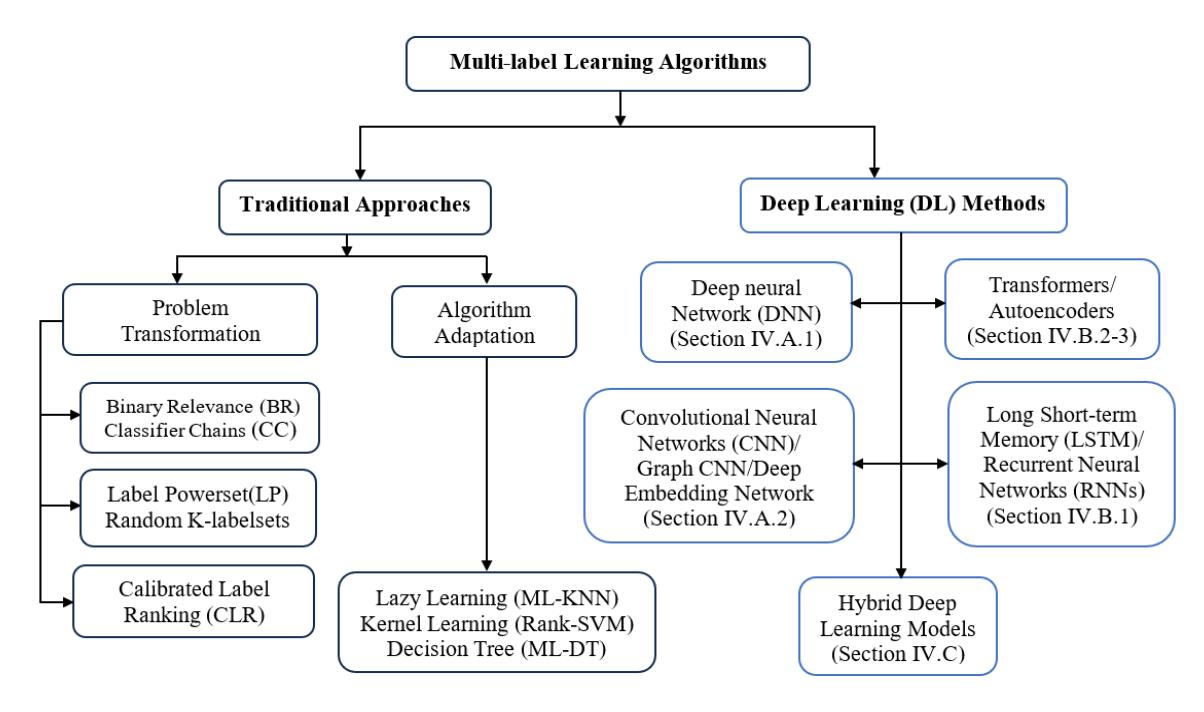
\includegraphics[width=0.88\textwidth]{figures/dl_mlc_taxonomy.jpeg}
    \caption{Phân loại tổng quát các hướng tiếp cận trong multi-label learning: nhóm truyền thống và nhóm Deep Learning.}
    \label{fig:dl_mlc_taxonomy}
\end{figure}

\subsection{Đầu ra và hàm mất mát trong mạng nơ-ron}

Ở các phần trước, bài toán phân loại đa lớp đã được mô tả thông qua hàm điểm số
$h(x,y)$ và quy tắc chọn nhãn có điểm số lớn nhất. Trong mạng nơ-ron, tầng cuối
thường sinh ra một vector điểm số chưa chuẩn hóa, gọi là \textit{logits}. Cách chuyển
logits thành dự đoán phụ thuộc vào việc bài toán là đơn nhãn hay đa nhãn.

Với bài toán multi-class đơn nhãn, mỗi mẫu chỉ thuộc đúng một lớp trong
$\{1,2,\ldots,k\}$. Vì các lớp loại trừ nhau, tầng đầu ra thường dùng softmax:
\[
    p(y=l\mid x)
    =
    \frac{\exp(z_l)}
    {\sum_{j=1}^{k}\exp(z_j)},
    \qquad l=1,\ldots,k.
\]
Khi đó, các xác suất trên $k$ lớp có tổng bằng $1$ và mô hình dự đoán lớp có xác
suất lớn nhất:
\[
    \hat{y}=\arg\max_{l} p(y=l\mid x).
\]
Hàm mất mát thường dùng là cross-entropy đa lớp:
\[
    \mathcal{L}_{CE}
    =
    -\frac{1}{m}
    \sum_{i=1}^{m}
    \log p(y_i\mid x_i).
\]

Với bài toán multi-label, một mẫu có thể đồng thời mang nhiều nhãn. Do đó, các nhãn
không được chuẩn hóa cạnh tranh như softmax. Nếu có $L$ nhãn, tầng đầu ra thường
gồm $L$ nút sigmoid:
\[
    p_{il}
    =
    \sigma(z_{il})
    =
    \frac{1}{1+\exp(-z_{il})},
    \qquad l=1,\ldots,L.
\]
Mỗi $p_{il}$ biểu diễn xác suất mẫu $x_i$ mang nhãn $l$. Nhãn dự đoán thường được
xác định bằng một ngưỡng $\tau_l$:
\[
    \hat{y}_{il}
    =
    \begin{cases}
    1, & p_{il}\geq \tau_l,\\
    0, & p_{il}<\tau_l.
    \end{cases}
\]
Hàm mất mát phổ biến là binary cross-entropy theo từng nhãn:
\[
    \mathcal{L}_{BCE}
    =
    -\frac{1}{m}
    \sum_{i=1}^{m}
    \sum_{l=1}^{L}
    \left[
    y_{il}\log(p_{il})
    +
    (1-y_{il})\log(1-p_{il})
    \right].
\]

Lưu ý rằng đầu ra sigmoid chỉ xem mỗi nhãn như một quyết định nhị phân ở tầng
cuối. Điều này không có nghĩa toàn bộ mô hình học các nhãn hoàn toàn tách rời. Trong
mạng nơ-ron, các tầng ẩn phía trước vẫn được học chung, nên mô hình có thể chia sẻ
biểu diễn giữa những nhãn có liên quan. Nếu muốn khai thác quan hệ nhãn rõ hơn,
các kiến trúc như attention, RNN/LSTM, Transformer hoặc graph thường được đặt ở
phần encoder trước khi đưa ra dự đoán cuối cùng.

\begin{table}[htbp]
\centering
\small
\renewcommand{\arraystretch}{1.25}
\begin{tabular}{p{0.23\textwidth} p{0.34\textwidth} p{0.33\textwidth}}
\hline
\textbf{Thiết lập}
& \textbf{Tầng đầu ra và loss}
& \textbf{Ý nghĩa dự đoán} \\
\hline

Multi-class đơn nhãn
&
Softmax trên $k$ lớp, thường dùng cross-entropy đa lớp.
&
Các lớp loại trừ nhau. Mỗi mẫu được gán đúng một nhãn bằng quy tắc
$\hat{y}=\arg\max_l p_l$. \\

\hline

Multi-label cơ bản
&
Sigmoid riêng cho từng nhãn, thường dùng binary cross-entropy theo từng nhãn.
&
Mỗi nhãn là một quyết định nhị phân. Một mẫu có thể đồng thời nhận nhiều nhãn
nếu $p_l \geq \tau_l$. \\

\hline

Multi-label có mô hình hóa quan hệ nhãn
&
Dùng encoder chung, attention, RNN/LSTM, Transformer hoặc graph trước tầng
sigmoid/ranking.
&
Mô hình không chỉ học đặc trưng đầu vào mà còn khai thác quan hệ đồng xuất hiện,
thứ tự hoặc cấu trúc giữa các nhãn. \\

\hline
\end{tabular}
\caption{So sánh tầng đầu ra của mạng nơ-ron trong bài toán multi-class và multi-label.}
\label{tab:dl_output_layer}
\end{table}

\subsection{Các kiến trúc học sâu tiêu biểu}

\paragraph{Mạng truyền thẳng và BP-MLL.}
Cách mở rộng đơn giản nhất là dùng một mạng nhiều tầng với $q$ nút đầu ra, mỗi nút tương ứng với một nhãn. Mô hình BP-MLL là một trong những hướng đầu tiên áp dụng mạng nơ-ron cho multi-label classification. Thay vì chỉ đo sai số từng nhãn riêng lẻ, BP-MLL tối ưu sao cho điểm của các nhãn đúng cao hơn điểm của các nhãn sai. Cách làm này phù hợp để minh họa bước chuyển từ các bộ phân loại nhị phân độc lập sang một mô hình học chung nhiều đầu ra.

\begin{figure}[htbp]
    \centering
    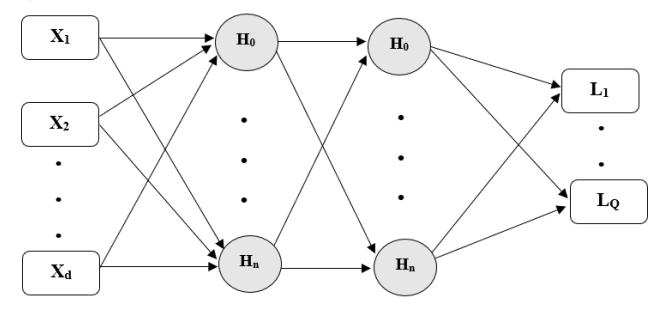
\includegraphics[width=0.68\textwidth]{figures/dl_mlc_dnn.jpeg}
    \caption{Mạng nơ-ron truyền thẳng cho multi-label classification: các đặc trưng đầu vào được ánh xạ qua tầng ẩn đến nhiều nút đầu ra, mỗi nút tương ứng với một nhãn.}
    \label{fig:dl_mlc_dnn}
\end{figure}

\paragraph{CNN và Graph CNN.}
CNN phù hợp với dữ liệu có cấu trúc cục bộ như ảnh, văn bản ngắn hoặc tín hiệu. Trong ảnh đa nhãn, một ảnh có thể chứa nhiều đối tượng cùng lúc, nên CNN thường được dùng làm bộ trích xuất đặc trưng, sau đó tầng đầu ra sigmoid dự đoán xác suất cho từng nhãn. Một số mô hình mở rộng dùng Graph CNN, trong đó mỗi nhãn được xem như một nút trong đồ thị; cạnh giữa các nút biểu diễn quan hệ đồng xuất hiện hoặc quan hệ ngữ nghĩa giữa các nhãn. Cách này giúp mô hình hóa tốt hơn các phụ thuộc nhãn mà CNN thông thường chưa xử lý trực tiếp.

\begin{figure}[htbp]
    \centering
    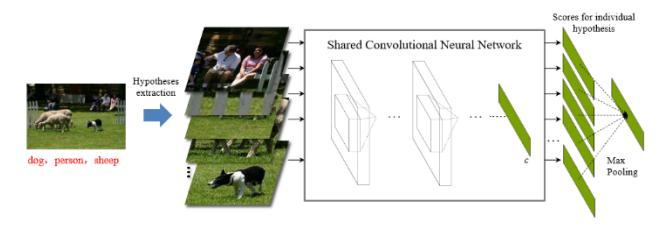
\includegraphics[width=0.82\textwidth]{figures/dl_mlc_cnn_hcp.jpeg}
    \caption{Minh họa hướng dùng CNN cho phân loại ảnh đa nhãn: các vùng/giả thuyết đối tượng được đưa qua CNN dùng chung, sau đó tổng hợp điểm để dự đoán nhiều nhãn.}
    \label{fig:dl_mlc_cnn_hcp}
\end{figure}

\paragraph{RNN/LSTM, Transformer và mô hình lai.}
RNN và LSTM phù hợp với dữ liệu tuần tự như văn bản, chuỗi thời gian hoặc tín hiệu y sinh. Trong multi-label classification, LSTM có thể được dùng để sinh chuỗi nhãn, trong đó nhãn dự đoán trước ảnh hưởng đến nhãn dự đoán sau. Ý tưởng này gần với Classifier Chains, nhưng thay vì dùng nhiều bộ phân loại rời rạc, mô hình học phụ thuộc nhãn trong một kiến trúc tuần tự duy nhất.

\[
    p(y \mid x) = \prod_{t=1}^{n}p(y_t \mid y_1, y_2,\ldots,y_{t-1},x).
\]

Transformer mở rộng hướng này bằng cơ chế attention, cho phép mô hình tập trung vào những phần khác nhau của đầu vào khi dự đoán từng nhãn. Trong xử lý văn bản, các mô hình dựa trên BERT thường cho biểu diễn ngữ cảnh tốt hơn CNN/RNN truyền thống. Trong thị giác máy tính, Transformer hoặc các mô hình lai CNN--Transformer có thể học đồng thời quan hệ không gian giữa vùng ảnh và quan hệ ngữ nghĩa giữa nhãn.

\begin{figure}[htbp]
    \centering
    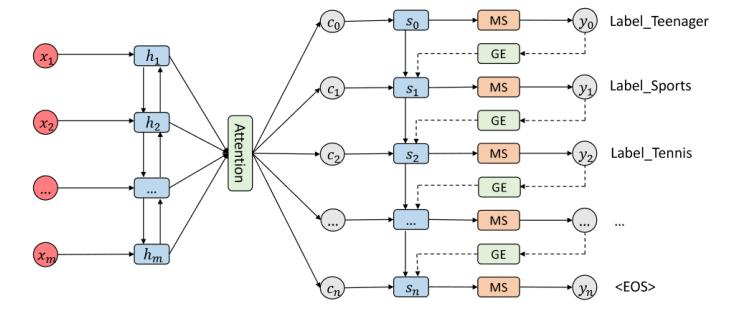
\includegraphics[width=0.82\textwidth]{figures/dl_mlc_lstm_seq.jpeg}
    \caption{Mô hình sinh chuỗi nhãn dùng RNN/LSTM: nhãn ở bước sau được dự đoán dựa trên đầu vào và các nhãn đã sinh trước đó.}
    \label{fig:dl_mlc_lstm_seq}
\end{figure}

\subsection{Liên hệ với các phương pháp truyền thống}

Deep Learning không thay thế hoàn toàn SVM, Decision Tree, OVA hay ECOC trong mọi trường hợp. Khi dữ liệu nhỏ, đặc trưng rõ ràng và yêu cầu diễn giải cao, các mô hình truyền thống vẫn phù hợp. Tuy nhiên, trong những bài toán có dữ liệu phi cấu trúc, quan hệ nhãn phức tạp hoặc số nhãn lớn, mạng nơ-ron thường linh hoạt hơn vì vừa học đặc trưng đầu vào, vừa học biểu diễn dùng chung cho nhiều nhãn.

\begin{table}[H]
\centering
\small
\renewcommand{\arraystretch}{1.25}
\begin{tabular}{p{0.22\textwidth} p{0.34\textwidth} p{0.34\textwidth}}
\hline
\textbf{Hướng tiếp cận} & \textbf{Vai trò } & \textbf{Giới hạn} \\
\hline
SVM, OVA & Nền tảng tuyến tính/kernel, dễ phân tích bằng lề và độ phức tạp. & Khó học quan hệ nhãn nếu các bộ phân loại được học độc lập. \\
Decision Tree & Dễ diễn giải, dự đoán nhanh. & Dễ overfit và không ổn định khi dữ liệu thay đổi. \\
AdaBoost.MH & Xử lý trực tiếp các cặp mẫu--nhãn trong thiết lập đa nhãn. & Chi phí tăng theo số mẫu nhân với số nhãn. \\
DNN/ CNN/ LSTM/ Transformer & Học biểu diễn đầu vào và biểu diễn nhãn trong cùng một mô hình. & Cần nhiều dữ liệu, tốn tài nguyên và khó giải thích hơn. \\
\hline
\end{tabular}
\caption{Liên hệ giữa các phương pháp truyền thống và học sâu trong phân loại đa lớp/đa nhãn.}
\label{tab:traditional_vs_dl}
\end{table}

\subsection{Nhận xét tổng quan}

Vai trò của Deep Learning trong bài toán multi-class/multi-label thể hiện ở hai khía cạnh chính. Thứ nhất, mạng nơ-ron có khả năng tự học biểu diễn đặc trưng từ dữ liệu, thay vì phụ thuộc nhiều vào đặc trưng thủ công như các phương pháp truyền thống. Thứ hai, trong bài toán đa nhãn, các tầng ẩn dùng chung cho phép mô hình chia sẻ thông tin giữa các nhãn; khi kết hợp thêm attention, RNN/LSTM, Transformer hoặc đồ thị nhãn, mô hình có thể khai thác tốt hơn quan hệ đồng xuất hiện, thứ tự hoặc cấu trúc giữa các nhãn.

Tuy nhiên, học sâu không loại bỏ hoàn toàn các khó khăn của bài toán. Các mô hình này thường cần nhiều dữ liệu huấn luyện, chi phí tính toán cao, khó diễn giải hơn so với cây quyết định hoặc mô hình tuyến tính, và vẫn gặp trở ngại khi số lượng nhãn tăng lên quy mô rất lớn. Vì vậy, trong các bài toán extreme multi-label, Deep Learning thường cần được kết hợp với các kỹ thuật giảm không gian nhãn, tạo shortlist hoặc tổ chức nhãn theo cây để đảm bảo khả năng mở rộng.

\section{Các nghiên cứu tiên tiến trong phân loại đa lớp cực đại}

\subsection{Tổng quan Extreme Multi-label Classification}

Trong thực tế, khi số lượng nhãn tăng lên quy mô hàng trăm nghìn hoặc hàng triệu, các thuật toán nền tảng như Multi-class SVM, One-versus-All (OVA) hoặc One-versus-One (OVO) gặp giới hạn nghiêm trọng về chi phí tính toán. Nếu số nhãn là $L$, việc đánh giá trực tiếp hàm điểm cho toàn bộ nhãn thường có độ phức tạp $O(L)$ cho mỗi mẫu, chưa kể chi phí huấn luyện và lưu trữ mô hình.

Extreme Multi-label Classification (XMC) được nghiên cứu nhằm giải quyết tình huống này. Trong XMC, mỗi mẫu có thể gắn với nhiều nhãn, nhưng số nhãn đúng thường rất nhỏ so với tổng số nhãn. Vì vậy, ma trận nhãn có dạng rất thưa và phân phối nhãn thường có tính đuôi dài: một số ít nhãn xuất hiện thường xuyên, trong khi phần lớn nhãn chỉ xuất hiện ở số lượng mẫu hạn chế.

Các thách thức chính của XMC gồm:
\begin{itemize}[leftmargin=2em]
  \item \textbf{Chi phí tính toán:} đánh giá toàn bộ $L$ nhãn là không khả thi khi $L$ rất lớn.
  \item \textbf{Nhãn đuôi:} các nhãn hiếm khó học vì có ít ví dụ huấn luyện.
  \item \textbf{Mất cân bằng dữ liệu:} mô hình dễ thiên về các nhãn phổ biến nếu chỉ tối ưu loss thông thường.
  \item \textbf{Biểu diễn ngữ nghĩa:} Bag-of-Words hoặc TF-IDF có thể không đủ để nắm bắt ngữ cảnh sâu của văn bản.
  \item \textbf{Triển khai thực tế:} hệ thống cần dự đoán nhanh, cập nhật nhãn mới và xử lý văn bản dài.
\end{itemize}

Phần này phân tích một số hướng nghiên cứu tiên tiến giai đoạn 2019--2024, tập trung vào cách các phương pháp hiện đại kế thừa, mở rộng và khắc phục giới hạn của lý thuyết nền tảng về phân loại đa lớp.
\begin{figure}[H]
\centering
\resizebox{0.98\textwidth}{!}{\begin{tikzpicture}[>=Stealth, font=\small]
  \node[align=center, font=\bfseries] at (4.6,4.85) {Phân phối đuôi dài của nhãn};
  \draw[->, thick] (0,0) -- (9.25,0) node[right] {Chỉ số nhãn};
  \draw[->, thick] (0,0) -- (0,4.35) node[above] {Tần suất};
  \fill[blue!10] (0.25,4.0) .. controls (0.8,1.05) and (2.4,0.45) .. (8.6,0.12) -- (8.6,0) -- (0.25,0) -- cycle;
  \draw[very thick, blue] (0.25,4.0) .. controls (0.8,1.05) and (2.4,0.45) .. (8.6,0.12);
  \draw[dashed, thick, red] (3.05,0) -- (3.05,4.05);
  \node[draw, rounded corners, fill=white, align=center, font=\scriptsize, inner sep=1.5pt, text width=1.75cm] (headnote) at (2.0,3.75) {Head labels\\xuất hiện thường xuyên};
  \draw[->, thick, blue!60!black] (headnote.south west) -- (0.55,3.55);
  \node[draw, rounded corners, fill=white, align=center, text=red!75!black, font=\scriptsize, inner sep=1.5pt, text width=1.8cm] at (6.7,2.75) {Tail labels\\nhiều nhãn hiếm};
  \draw[<->, red!70!black, thick] (3.25,1.45) -- (8.6,1.45) node[midway, above, fill=white, font=\scriptsize, inner sep=1pt] {phần lớn không gian nhãn};
  \node[left, font=\scriptsize] at (0,4.0) {$10^4$};
  \node[left, font=\scriptsize] at (0,2.0) {$10^2$};
  \node[left, font=\scriptsize] at (0,0.1) {$10^0$};
  \node[below, font=\scriptsize] at (8.6,0) {325K};
\end{tikzpicture}}
\caption{Phân phối đuôi dài của nhãn trong bài toán phân loại đa nhãn cực lớn.}
\label{fig:xmc-long-tail}
\end{figure}


\subsection{Phân tích các bài báo tiêu biểu}

\subsubsection{Bonsai: Diverse and shallow trees for XMC}

\paragraph{Bài toán đặt ra.} Bonsai là một phương pháp cây nông đa dạng cho XMC \cite{khandagale2020bonsai}.
Các phương pháp dựa trên cây trước đây, chẳng hạn Parabel, thường ép cây phải phân chia nhị phân và cân bằng. Ràng buộc này làm cây trở nên sâu khi số nhãn lớn. Cây càng sâu thì lỗi ở các nút gần gốc càng dễ lan truyền xuống các tầng dưới, gây hiện tượng error propagation. Một khi mẫu đi nhầm nhánh, các nhãn đúng ở nhánh khác có thể không bao giờ được xét đến. Điều này đặc biệt bất lợi với các nhãn đuôi hiếm gặp.

\paragraph{Đóng góp chính.}
Bonsai nới lỏng ràng buộc cân bằng và cho phép phân chia đa phân (K-way partitioning), trong đó $K$ có thể rất lớn, ví dụ $K\geq 100$. Thay vì ép mỗi nút chia thành hai nhánh cân bằng, Bonsai dùng phân cụm như K-means để tạo ra các cây nông và đa dạng. Cây nông giúp giảm số bước quyết định từ gốc đến lá, nhờ đó giảm nguy cơ lỗi lan truyền. Tính đa dạng của nhiều cây giúp cải thiện khả năng bao phủ nhãn đuôi.
\begin{figure}[H]
\centering
\resizebox{0.98\textwidth}{!}{\begin{tikzpicture}[>=Stealth, font=\small]
  \node[align=center, font=\bfseries] at (4,4.25) {Parabel vs. Bonsai trong phân hoạch nhãn};
  \begin{scope}[shift={(1.4,0)}]
    \node[align=center, font=\bfseries] at (0,3.05) {Parabel\\cây nhị phân};
    \node[circle, draw, thick, fill=blue!20, minimum size=1.0cm] (p0) at (0,1.8) {};
    \node[circle, draw, thick, fill=blue!15, minimum size=0.75cm] (p1) at (-1.05,0.65) {};
    \node[circle, draw, thick, fill=blue!15, minimum size=0.75cm] (p2) at (1.05,0.65) {};
    \foreach \x/\n in {-1.55/p3,-0.55/p4,0.55/p5,1.55/p6} {\node[circle, draw, thick, fill=blue!10, minimum size=0.42cm] (\n) at (\x,-0.65) {};}
    \draw[->, thick] (p0)--(p1); \draw[->, thick] (p0)--(p2);
    \draw[->, thick] (p1)--(p3); \draw[->, thick] (p1)--(p4);
    \draw[->, thick] (p2)--(p5); \draw[->, thick] (p2)--(p6);
    \node[align=center, text=blue!80!black, font=\footnotesize] at (0,-1.65) {Nhiều tầng quyết định\\dễ lan truyền lỗi};
  \end{scope}
  \draw[dashed, thick, gray] (4,3.45) -- (4,-1.95);
  \begin{scope}[shift={(6.5,0)}]
    \node[align=center, font=\bfseries] at (0,3.05) {Bonsai\\cây đa phân nông};
    \node[circle, draw, thick, fill=green!20, minimum size=1.0cm] (b0) at (0,1.65) {};
    \node[circle, draw, thick, fill=green!15, minimum size=0.86cm] (b1) at (-1.65,0.25) {};
    \node[circle, draw, thick, fill=green!15, minimum size=0.58cm] (b2) at (0,0.25) {};
    \node[circle, draw, thick, fill=green!15, minimum size=0.72cm] (b3) at (1.65,0.25) {};
    \draw[->, thick] (b0)--(b1); \draw[->, thick] (b0)--(b2); \draw[->, thick] (b0)--(b3);
    \node[align=center, text=green!55!black, font=\footnotesize] at (0,-1.65) {Ít tầng hơn\\giữ recall cho nhãn đuôi};
  \end{scope}
\end{tikzpicture}}
\caption{Ý tưởng cây nông đa phân trong Bonsai nhằm giảm lỗi lan truyền.}
\label{fig:xmc-bonsai-tree}
\end{figure}


\paragraph{Liên hệ với lý thuyết nền tảng.}
Bonsai phát triển trực tiếp từ tư tưởng cây quyết định đã trình bày trong nhóm thuật toán không kết hợp. Tuy nhiên, thay vì phân hoạch không gian đặc trưng bằng greedy split dựa trên node impurity như Gini hoặc Entropy, Bonsai phân hoạch \textbf{không gian nhãn}. Việc phân hoạch có thể dựa trên biểu diễn đầu vào, biểu diễn đầu ra hoặc biểu diễn kết hợp. Như vậy, Bonsai giữ lại ưu điểm tính toán của cây nhưng điều chỉnh cấu trúc cây để phù hợp với bài toán XMC.

\paragraph{Nhận xét.}
Ưu điểm của Bonsai là giảm chiều sâu cây, tăng khả năng bảo toàn nhãn đuôi và cải thiện tốc độ dự đoán. Hạn chế là mô hình vẫn có thể chịu lỗi lan truyền ở các nút cao; ngoài ra chất lượng phân cụm nhãn ảnh hưởng mạnh đến chất lượng dự đoán cuối cùng.

\subsubsection{LightXML: Transformer with Dynamic Negative Sampling}

\paragraph{Bài toán đặt ra.}
Các mô hình học sâu cho XMC thường phải xử lý số nhãn âm cực lớn. Nếu dùng static negative sampling, mô hình chỉ nhìn thấy một nhóm nhãn âm cố định hoặc ít thay đổi, dẫn đến nguy cơ overfit vào các nhãn âm cụ thể và khó học được ranh giới tốt giữa nhãn đúng và nhãn sai khó. Ngoài ra, huấn luyện Transformer trên không gian nhãn cực lớn đòi hỏi tài nguyên tính toán rất cao.

\paragraph{Đóng góp chính.}
LightXML sử dụng mạng hợp tác sinh--phân biệt (generative cooperative networks). Bộ tạo (Generator) có nhiệm vụ gọi lại một tập nhãn ứng viên, đóng vai trò như cơ chế lấy mẫu tiêu cực động. Ở giai đoạn đầu, Generator có thể cung cấp các nhãn âm dễ; khi mô hình tốt hơn, nó sinh ra các nhãn âm khó hơn. Bộ phân biệt (Discriminator) sau đó xếp hạng các nhãn trong tập ứng viên này.
\begin{figure}[H]
\centering
\resizebox{0.98\textwidth}{!}{\begin{tikzpicture}[>=Stealth, font=\footnotesize]
  \node[align=center, font=\bfseries] at (4.5,3.45) {LightXML: lấy mẫu tiêu cực động};
  \node[draw, thick, fill=cyan!10, rectangle, rounded corners, minimum width=2.25cm, minimum height=1.05cm, align=center] (gen) at (0.35,1.35) {Generator\\gọi lại nhãn};
  \node[draw, dashed, thick, fill=yellow!12, rounded corners, minimum width=2.35cm, minimum height=1.05cm, align=center] (cand) at (4.5,1.35) {Tập ứng viên\\hard negatives};
  \node[draw, thick, fill=magenta!10, rectangle, rounded corners, minimum width=2.25cm, minimum height=1.05cm, align=center] (disc) at (8.65,1.35) {Discriminator\\xếp hạng nhãn};

  \draw[->, very thick, blue] (gen.east) -- (cand.west);
  \draw[->, very thick, blue] (cand.east) -- (disc.west);
  \node[font=\tiny, text=blue, fill=white, inner sep=1pt] at (2.42,1.92) {sinh nhãn khó};
  \node[font=\tiny, text=blue, fill=white, inner sep=1pt] at (6.58,1.92) {lọc và xếp hạng};

  \draw[->, thick, red!75!black, dashed] (disc.south) |- (4.5,-0.15) -| (gen.south);
  \node[font=\tiny, text=red!75!black, fill=white, inner sep=1pt] at (2.2,-0.28) {tối ưu hóa chung};

  \node[draw, rounded corners, fill=white, align=center, font=\footnotesize, text width=7.2cm] at (4.5,-1.15) {Generator liên tục tạo nhãn âm khó hơn, giúp Discriminator học ranh giới tốt hơn trên không gian nhãn lớn.};
\end{tikzpicture}}
\caption{Cơ chế lấy mẫu tiêu cực động trong LightXML với Generator và Discriminator.}
\label{fig:xmc-lightxml}
\end{figure}


\paragraph{Liên hệ với lý thuyết nền tảng.}
Về bản chất, phần xếp hạng của LightXML vẫn tương đồng với chiến lược OVA: mỗi nhãn được xem như một bài toán nhị phân độc lập và dùng loss nhị phân cho từng nhãn. Điểm khác biệt là LightXML không đánh giá toàn bộ $L$ nhãn. Generator thu gọn không gian nhãn từ $O(L)$ xuống một shortlist nhỏ, giúp giảm đáng kể chi phí tính toán.

\paragraph{Nhận xét.}
LightXML kế thừa sức mạnh biểu diễn của Transformer và giải quyết nút thắt nhãn âm bằng dynamic negative sampling. Tuy nhiên, phương pháp vẫn phụ thuộc vào giới hạn chiều dài đầu vào của Transformer và chất lượng shortlist do Generator tạo ra.

\subsubsection{XR-Transformer: Fast Multi-Resolution Fine-tuning}

\paragraph{Bài toán đặt ra.} XR-Transformer đề xuất fine-tuning Transformer đa độ phân giải cho XMC \cite{zhang2021xrtransformer}.
Fine-tuning trực tiếp các mô hình Transformer lớn như BERT hoặc RoBERTa trên hàng trăm nghìn đến hàng triệu nhãn là rất tốn thời gian. Nếu mỗi bước phải tính điểm cho toàn bộ nhãn, độ phức tạp tuyến tính theo $L$ khiến huấn luyện có thể kéo dài nhiều ngày hoặc nhiều tuần.

\paragraph{Đóng góp chính.}
XR-Transformer chia bài toán thành nhiều độ phân giải thông qua cây nhãn phân cấp (Hierarchical Label Tree -- HLT). Mô hình được fine-tune theo chiến lược coarse-to-fine: trước hết học ở mức cụm nhãn thô, sau đó tinh chỉnh dần xuống các cụm nhỏ hơn và cuối cùng đến nhãn cụ thể. Ngoài ra, để bù đắp thông tin bị mất do Transformer phải cắt cụt văn bản, XR-Transformer kết hợp đặc trưng ngữ nghĩa từ Transformer với đặc trưng thưa TF-IDF.

\paragraph{Liên hệ với lý thuyết nền tảng.}
XR-Transformer giải quyết trực tiếp thách thức chi phí tính toán trong phân loại đa lớp cực đại. Bằng cách biến phân loại phẳng trên $L$ nhãn thành phân loại theo cây, phương pháp giảm số nhãn cần xét ở mỗi bước. Trong điều kiện cây được tổ chức tốt, chi phí dự đoán có thể giảm từ $O(L)$ xuống gần $O(\log L)$ hoặc phụ thuộc vào kích thước shortlist ở từng tầng.

\paragraph{Nhận xét.}
Điểm mạnh của XR-Transformer là kết hợp ba thành phần: Transformer để học ngữ nghĩa, TF-IDF để giữ tín hiệu thống kê thưa, và cây nhãn để tăng tốc. Hạn chế là chất lượng cây nhãn ảnh hưởng lớn đến kết quả; nếu mẫu bị đưa sai nhánh ở tầng thô, nhãn đúng có thể bị loại khỏi các bước tinh hơn.

\subsubsection{ICXML: In-Context Learning for Zero-shot XMC}

\paragraph{Bài toán đặt ra.} ICXML là khung in-context learning cho zero-shot XMC \cite{zhu2024icxml}.
Trong nhiều hệ thống thực tế, nhãn mới có thể xuất hiện mà không có dữ liệu huấn luyện đi kèm. Đây là thiết lập zero-shot XMC. Một cách tự nhiên là dùng mô hình ngôn ngữ lớn (LLM), nhưng không thể đưa hàng trăm nghìn hoặc hàng triệu nhãn vào prompt vì giới hạn độ dài ngữ cảnh.

\paragraph{Đóng góp chính.}
ICXML đề xuất khung gồm hai giai đoạn: Generate và Rerank. Ở giai đoạn Generate, LLM tạo các pseudo-demonstrations hoặc tín hiệu ngữ nghĩa để sinh ra danh sách nhãn rút gọn. Ở giai đoạn Rerank, LLM thực hiện phân loại đa nhãn trên shortlist này bằng in-context learning. Nhờ đó, hệ thống không cần huấn luyện lại toàn bộ mô hình cho các nhãn mới.

\paragraph{Liên hệ với lý thuyết nền tảng.}
ICXML khác với giả định cổ điển của phân loại có giám sát, trong đó mô hình học tham số từ tập huấn luyện có nhãn $(\bm{x}_i,y_i)$. Thay vì học các vector trọng số $\bm{w}_l$ như Multi-class SVM hoặc OVA, ICXML dựa vào tri thức nền và khả năng suy luận trong ngữ cảnh của LLM. Tuy nhiên, nó vẫn cần cơ chế rút gọn nhãn vì không gian nhãn đầy đủ quá lớn.

\paragraph{Nhận xét.}
ICXML mở ra hướng zero-shot cho XMC, đặc biệt hữu ích khi nhãn thay đổi nhanh. Hạn chế là chi phí suy luận của LLM cao, kết quả phụ thuộc mạnh vào prompt, và mô hình có thể sinh hoặc chọn nhãn không nhất quán nếu shortlist không được kiểm soát tốt.

\subsection{Đánh giá xu hướng phát triển}

Sự dịch chuyển từ lý thuyết phân loại đa lớp nền tảng sang XMC hiện đại thể hiện qua ba xu hướng chính.

\subsubsection{Từ đặc trưng thưa sang ngữ nghĩa sâu}

Các thuật toán truyền thống thường dựa trên Bag-of-Words hoặc TF-IDF. Những đặc trưng này có ưu điểm là thưa, dễ tính và mở rộng tốt, nhưng khó nắm bắt ngữ cảnh dài, đồng nghĩa và quan hệ ngữ nghĩa phức tạp. Các phương pháp hiện đại chuyển sang dùng BiLSTM, attention và Transformer để học biểu diễn ngữ nghĩa sâu. AttentionXML dùng BiLSTM và attention đa nhãn \cite{you2019attentionxml}; LightXML và XR-Transformer dùng Transformer để học biểu diễn văn bản theo ngữ cảnh.
\begin{figure}[H]
\centering
\resizebox{0.98\textwidth}{!}{\begin{tikzpicture}[>=Stealth, font=\small]
  \node[align=center, font=\bfseries] at (4,5.75) {AttentionXML: attention riêng cho từng nhãn};
  \node[draw, thick, fill=gray!10, minimum width=5.8cm, minimum height=0.62cm] (text) at (4,0) {Văn bản đầu vào};
  \node[draw, thick, fill=blue!10, minimum width=5.8cm, minimum height=0.62cm] (emb) at (4,1.05) {Word representation};
  \node[draw, thick, fill=orange!10, minimum width=5.8cm, minimum height=0.62cm] (bilstm) at (4,2.1) {BiLSTM};
  \node[draw, thick, fill=purple!10, minimum width=6.6cm, minimum height=0.95cm, align=center] (att) at (4,3.35) {Multi-label attention\\hệ số $\alpha_{ij}$ phụ thuộc từng nhãn};
  \node[draw, thick, fill=green!10, minimum width=2.25cm, minimum height=0.66cm] (fc1) at (1.55,5.05) {Nhãn A};
  \node[draw, thick, fill=green!10, minimum width=2.25cm, minimum height=0.66cm] (fc2) at (6.45,5.05) {Nhãn B};
  \draw[->, thick] (text)--(emb); \draw[->, thick] (emb)--(bilstm); \draw[->, thick] (bilstm)--(att);
  \draw[->, thick] (att)--(fc1) node[pos=0.56, left, font=\scriptsize, fill=white, inner sep=1pt] {trọng số A};
  \draw[->, thick] (att)--(fc2) node[pos=0.56, right, font=\scriptsize, fill=white, inner sep=1pt] {trọng số B};
\end{tikzpicture}}
\caption{Cơ chế attention đa nhãn trong AttentionXML.}
\label{fig:xmc-attentionxml}
\end{figure}


Tuy vậy, đặc trưng thưa chưa biến mất hoàn toàn. XR-Transformer cho thấy TF-IDF vẫn hữu ích khi kết hợp với Transformer, đặc biệt vì TF-IDF giữ lại tín hiệu từ toàn bộ văn bản trong khi Transformer thường bị giới hạn độ dài đầu vào.

\subsubsection{Cấu trúc cây vẫn là cốt lõi của tính toán}

Dù mô hình học sâu có năng lực biểu diễn cao hơn, việc đánh giá hàm điểm trên hàng triệu nhãn vẫn là điểm nghẽn tính toán. Vì vậy, cấu trúc cây tiếp tục đóng vai trò trung tâm. Bonsai dùng cây nông đa dạng để giảm lỗi lan truyền; AttentionXML kết hợp attention với cây nhãn xác suất; XR-Transformer dùng cây nhãn phân cấp để fine-tune theo nhiều độ phân giải.

Điểm chung là các phương pháp này không cố tính điểm cho mọi nhãn. Thay vào đó, chúng dùng cây để tạo shortlist hoặc dẫn đường quá trình dự đoán, từ đó đưa độ phức tạp từ tuyến tính theo $L$ về mức gần logarit hoặc theo kích thước tập ứng viên nhỏ.

\subsubsection{Tập trung vào phân phối đuôi dài}

Vấn đề mất cân bằng lớp trong lý thuyết nền tảng trở nên nghiêm trọng hơn nhiều trong XMC. Phần lớn nhãn là tail labels, có rất ít mẫu huấn luyện. Nếu chỉ tối ưu các thước đo thông thường, mô hình dễ đạt kết quả tốt trên nhãn phổ biến nhưng bỏ qua nhãn hiếm.

Do đó, các nghiên cứu XMC thường dùng các thước đo như propensity-scored precision@k (PSP@k) hoặc propensity-scored nDCG. Ý tưởng là tăng trọng số đánh giá cho nhãn hiếm để phản ánh đúng giá trị của việc dự đoán tail labels. Xu hướng này cho thấy bài toán XMC không chỉ là bài toán tăng tốc tính toán, mà còn là bài toán học trong phân phối mất cân bằng cực đoan.

\begin{expandbox}
\subsection{Hạn chế của các phương pháp hiện tại và đề xuất cải tiến}

\subsubsection{Hạn chế hiện tại}

\paragraph{Giới hạn độ dài văn bản của Transformer.}
Các mô hình như XR-Transformer và LightXML thường phải cắt cụt đầu vào xuống 128 hoặc 512 token để tránh vượt bộ nhớ GPU. Nguyên nhân là cơ chế self-attention truyền thống có độ phức tạp $O(N^2)$ theo độ dài chuỗi $N$. Với các tài liệu dài như văn bản pháp luật, hồ sơ y khoa hoặc bài báo khoa học, việc cắt cụt làm mất nhiều thông tin ngữ nghĩa quan trọng.

\paragraph{Lỗi lan truyền trong cây.}
Mặc dù Bonsai dùng cây nông để giảm error propagation, sai số ở các nút gần gốc vẫn có thể khiến mẫu đi sai nhánh. Khi đó, nhãn đúng có thể bị loại khỏi quá trình xét về sau. Đây là hạn chế chung của các phương pháp dựa trên cây, đặc biệt khi mỗi bước chỉ giữ lại một số ít nhánh ứng viên.

\paragraph{Phụ thuộc vào shortlist.}
Nhiều hệ thống hiện đại dùng bước tạo shortlist trước khi rerank. Nếu shortlist không chứa nhãn đúng, bộ reranker có năng lực biểu diễn cao cũng không thể phục hồi kết quả. Vì vậy, recall của bước tạo ứng viên là yếu tố then chốt trong XMC.

\subsubsection{Đề xuất cải tiến}

\paragraph{Sử dụng kiến trúc có độ phức tạp tuyến tính.}
Một hướng cải tiến là thay Transformer truyền thống bằng các kiến trúc có độ phức tạp gần tuyến tính theo độ dài chuỗi, chẳng hạn Longformer, State Space Models hoặc Mamba. Các mô hình này cho phép xử lý văn bản dài hàng nghìn token mà không cần cắt cụt quá mạnh, từ đó giữ được nhiều thông tin hơn cho các nhãn đuôi.

\paragraph{Kết hợp XR-Transformer với đồ thị tri thức.}
XR-Transformer hiện bù đắp thông tin mất do cắt cụt bằng cách nối vector Transformer với vector TF-IDF. Một hướng mở rộng là bổ sung đồ thị tri thức biểu diễn quan hệ giữa các nhãn, ví dụ quan hệ phân cấp, đồng xuất hiện hoặc quan hệ ngữ nghĩa. Graph Neural Networks (GNNs) có thể học embedding nhãn từ đồ thị này, sau đó kết hợp với đặc trưng văn bản để tăng chất lượng dự đoán.

Cách tiếp cận này đặc biệt hữu ích trong zero-shot XMC: ngay cả khi một nhãn mới chưa có dữ liệu huấn luyện, mô hình vẫn có thể tận dụng mô tả nhãn và quan hệ của nhãn đó trong đồ thị để suy luận. Điều này nối kết trực tiếp với vấn đề quan hệ phân cấp hoặc đồ thị giữa các lớp đã được nêu trong phần phát biểu bài toán.

\paragraph{Giảm lỗi lan truyền bằng multi-path routing.}
Thay vì ép mỗi mẫu đi theo một nhánh duy nhất trong cây, có thể cho phép multi-path routing, tức giữ lại nhiều nhánh ứng viên ở mỗi tầng. Cách này tăng chi phí dự đoán một phần, nhưng cải thiện recall của shortlist và giảm nguy cơ loại nhãn đúng quá sớm.

\paragraph{Kết hợp LLM với hệ thống truy hồi truyền thống.}
LLM mạnh trong zero-shot và hiểu ngữ nghĩa, nhưng chi phí suy luận cao. Do đó, một hướng thực tế là dùng mô hình truy hồi nhẹ để tạo shortlist lớn, sau đó dùng LLM rerank hoặc giải thích kết quả trên shortlist nhỏ. Cách kết hợp này cân bằng giữa tốc độ, khả năng mở rộng và chất lượng ngữ nghĩa.
\begin{figure}[H]
\centering
\resizebox{0.98\textwidth}{!}{\begin{tikzpicture}[>=Stealth, font=\small]
  \node[align=center, font=\bfseries] at (4,4.2) {Generate--rerank bằng LLM};
  \node[draw, thick, fill=gray!10, rounded corners, minimum width=2.2cm, minimum height=0.8cm, align=center] (input) at (0.6,2) {Văn bản\\đầu vào};
  \node[draw, thick, fill=blue!10, rounded corners, minimum width=2.55cm, minimum height=1.0cm, align=center] (gen) at (3.5,3) {Giai đoạn 1\\Generate};
  \node[draw, thick, fill=green!10, rounded corners, minimum width=2.25cm, minimum height=0.85cm, align=center] (space) at (6.8,3) {Không gian nhãn\\rút gọn};
  \node[draw, thick, fill=orange!10, rounded corners, minimum width=2.55cm, minimum height=1.0cm, align=center] (rerank) at (3.5,1) {Giai đoạn 2\\Rerank};
  \node[draw, thick, fill=red!10, rounded corners, minimum width=2.25cm, minimum height=0.85cm, align=center] (output) at (6.8,1) {Dự đoán\\cuối cùng};
  \draw[->, thick] (input) |- (gen.west);
  \draw[->, thick] (input) |- (rerank.west);
  \draw[->, thick] (gen)--(space) node[midway, above, font=\scriptsize, fill=white] {shortlist};
  \draw[->, thick] (space)--(rerank) node[midway, right, font=\scriptsize, fill=white] {ứng viên};
  \draw[->, thick] (rerank)--(output);
  \node[draw, rounded corners, fill=white, align=center, font=\footnotesize, text width=6.7cm] at (4,-0.45) {Mô hình truy hồi giảm không gian nhãn trước; LLM chỉ xếp hạng lại tập ứng viên nhỏ.};
\end{tikzpicture}}
\caption{Khung generate--rerank dùng LLM trên không gian nhãn đã rút gọn.}
\label{fig:xmc-llm-rerank}
\end{figure}

\section{Cải tiến của thuật toán cấu trúc: Kết hợp Mạng nơ-ron với CRF (Neural CRFs)}
\label{sec:neural_crfs}

\textit{Lưu ý: Mặc dù trong bảng phân công ghi là "Neural CFSs" nhưng xét theo ngữ cảnh của các thuật toán dự đoán cấu trúc (Structured Prediction) như CRFs ở phần trước, đây là chủ đề về Neural CRFs.}

\subsection{Động lực và bối cảnh}
\label{ssec:neural_crf_motivation}
Các thuật toán dự đoán cấu trúc cổ điển -- đặc biệt là CRF (Conditional Random Fields) \cite{lafferty2001conditional}, $M^3N$ \cite{taskar2003max}, và SVMStruct \cite{tsochantaridis2005large} -- đã đặt nền móng lý thuyết vững chắc cho bài toán gán nhãn chuỗi. Tuy nhiên, chúng chia sẻ một hạn chế chung: hàm tiềm năng (potential function) được xây dựng từ các đặc trưng thủ công do chuyên gia thiết kế, đòi hỏi nhiều công sức và khó chuyển đổi giữa các miền (domain).

Trong thập kỷ vừa qua, xu hướng chủ đạo trong Xử lý Ngôn ngữ Tự nhiên (NLP) là thay thế khâu trích xuất đặc trưng thủ công bằng mạng nơ-ron sâu, từ đó hình thành họ mô hình Neural CRF (Neural Conditional Random Fields). Ý tưởng cốt lõi rất tự nhiên: dùng mạng nơ-ron để tính hàm tiềm năng $\psi(\bm{x}_i, y_i)$ và $\psi(y_{i-1}, y_i)$ trong CRF thay vì dùng đặc trưng tuyến tính, trong khi vẫn giữ nguyên cơ chế suy luận toàn cục (global inference) của CRF qua thuật toán Viterbi và forward-backward. Nhờ đó, mô hình vừa có khả năng biểu diễn phi tuyến mạnh mẽ, vừa đảm bảo ràng buộc nhãn hợp lệ ở cấp độ chuỗi -- điều mà các mô hình phân loại độc lập từng vị trí không làm được.

\subsection{Kiến trúc BiLSTM-CRF -- Nền tảng của Neural CRF}
\label{ssec:bilstm_crf}
Một trong những mô hình Neural CRF có ảnh hưởng nhất là kiến trúc Bidirectional LSTM-CRF (BiLSTM-CRF) được đề xuất bởi Huang et al. \cite{huang2015bidirectional}. Kiến trúc này gồm hai thành phần chính:
\begin{enumerate}[leftmargin=2em]
    \item \textbf{Encoder BiLSTM:} Mạng LSTM hai chiều nhận chuỗi đầu vào $\bm{x} = (x_1, \ldots, x_n)$ và tạo ra vector ngữ cảnh $\bm{h}_i$ cho mỗi vị trí $i$, tích hợp thông tin từ cả quá khứ lẫn tương lai của chuỗi.
    \item \textbf{Decoder CRF:} Lớp CRF tuyến tính chuỗi (linear-chain CRF) ở tầng cuối mô hình hóa xác suất nhãn toàn chuỗi:
    \begin{equation}
        p(\bm{y}|\bm{x}) = \frac{1}{Z(\bm{x})} \exp\left( \sum_{i=1}^{n} \left[ A_{y_{i-1}, y_i} + \phi(\bm{h}_i, y_i) \right] \right)
        \label{eq:bilstm_crf_prob}
    \end{equation}
    trong đó $A \in \mathbb{R}^{|\mathcal{Y}| \times |\mathcal{Y}|}$ là ma trận chuyển tiếp nhãn được học, $\phi(\bm{h}_i, y_i)$ là điểm phát xạ (emission score) tính từ BiLSTM, và $Z(\bm{x})$ là hằng số phân hoạch.
\end{enumerate}

Kiến trúc này không chỉ đạt hiệu suất vượt trội trên các tác vụ NER và gán nhãn từ loại mà còn trở thành baseline chuẩn cho cộng đồng nghiên cứu NLP. Bước tiến tiếp theo là thay thế BiLSTM bằng BERT \cite{devlin2019bert} -- mô hình ngôn ngữ tiền huấn luyện dựa trên kiến trúc Transformer, tạo thành họ mô hình BERT-CRF với hiệu suất được cải thiện đáng kể do BERT cung cấp biểu diễn ngữ nghĩa phong phú hơn.

\begin{figure}[H]
\centering
% \resizebox{0.85\textwidth}{!}{\input{figures/bilstm_crf_architecture}}
\caption{Sơ đồ cấu trúc tầng trích xuất ngữ cảnh phi tuyến (BiLSTM/BERT) kết hợp tầng suy luận chuỗi toàn cục (CRF).}
\label{fig:bilstm_crf_layout}
\end{figure}

\subsection{Các bài báo tiêu biểu sau năm 2021}
\label{ssec:recent_crf_papers}
Phần này tóm tắt ba hướng nghiên cứu nổi bật về Neural CRF được công bố sau năm 2021, phản ánh sự phát triển đa dạng của lĩnh vực này.

\paragraph{Bài báo 1: Cải tiến lý thuyết cho dự đoán cấu trúc (NeurIPS 2023)}
\begin{itemize}[leftmargin=2em]
    \item \textbf{Tên bài báo:} \textit{Structured Prediction with Stronger Consistency Guarantees} \cite{mao2023structured}.
    \item \textbf{Tác giả:} Anqi Mao, Mehryar Mohri, Yutao Zhong.
    \item \textbf{Venue:} Advances in Neural Information Processing Systems 36 (NeurIPS 2023), Main Conference Track.
    \item \textbf{Vấn đề đặt ra:} Một điểm yếu ít được chú ý của CRF và các thuật toán dự đoán cấu trúc hiện đại là chúng tối thiểu hàm mất mát thay thế (surrogate loss) như cross-entropy hay soft-max thay vì trực tiếp tối thiểu mất mát Hamming -- vốn là mục tiêu thực sự. Câu hỏi đặt ra là: liệu việc tối thiểu surrogate loss có nhất quán Bayes (Bayes-consistent), tức là đảm bảo hội tụ về bộ phân loại Bayes tối ưu khi dữ liệu tăng vô hạn?
    \item \textbf{Đóng góp chính:} Nhóm tác giả -- đáng chú ý có Mehryar Mohri, đồng tác giả của sách giáo khoa FML \cite{mohri2018foundations} -- chứng minh rằng:
    \begin{enumerate}
        \item Không có cận $H$-nhất quán (H-consistency bound) không tầm thường nào có thể được thiết lập cho các surrogate loss phổ biến dùng trong dự đoán cấu trúc (như log-likelihood của CRF). Điều này có nghĩa là các đảm bảo lý thuyết của CRF truyền thống yếu hơn nhiều so với những gì thường được giả định.
        \item Nhóm tác giả đề xuất hai họ hàm mất mát mới: \textit{Structured comp-sum losses} (tổng quát hóa cross-entropy cho không gian đầu ra cấu trúc) và \textit{Structured constrained losses} (thiết kế đặc biệt để thỏa mãn ràng buộc nhất quán). Với cả hai họ, nhóm tác giả chứng minh được các cận $H$-nhất quán không tiệm cận, mạnh hơn và mang nhiều ý nghĩa thực tiễn hơn so với Bayes-consistency thuần túy.
    \end{enumerate}
    \item \textbf{Liên hệ với lý thuyết trong sách:} Kết quả này trực tiếp mở rộng phân tích về $M^3N$ và SVMStruct trong Chương 8 \cite{mohri2018foundations}. Các bài toán $M^3N$ và SVMStruct tối ưu hóa margin nhưng vẫn dùng surrogate -- bài báo này làm rõ khi nào surrogate đó đảm bảo nhất quán với bộ phân loại Bayes, một câu hỏi mà sách giáo khoa chỉ đề cập ngắn gọn.
\end{itemize}

\paragraph{Bài báo 2: Neural-Hidden-CRF cho giám sát yếu (KDD 2023)}
\begin{itemize}[leftmargin=2em]
    \item \textbf{Tên bài báo:} \textit{Neural-Hidden-CRF: A Robust Weakly-Supervised Sequence Labeler} \cite{chen2023neural_hidden_crf}.
    \item \textbf{Tác giả:} Zhijun Chen, Hailong Sun, Wanhao Zhang, Chunyi Xu, Qianren Mao, Pengpeng Chen.
    \item \textbf{Venue:} Proceedings of the 29th ACM SIGKDD Conference on Knowledge Discovery and Data Mining (KDD 2023).
    \item \textbf{Vấn đề đặt ra:} Trong thực tế, việc thu thập dữ liệu gán nhãn chất lượng cao rất tốn kém. Thay vào đó, người ta thường dùng giám sát yếu (weak supervision): nhãn được tạo tự động từ nhiều nguồn ồn ào (noisy labelers), ví dụ các hàm gán nhãn heuristic hoặc kết quả crowd-sourcing. Mô hình CRF truyền thống và BERT-CRF gặp khó khăn trong bối cảnh này vì chúng không mô hình hóa được sự không chắc chắn trong nhãn huấn luyện.
    \item \textbf{Kiến trúc đề xuất:} Neural-Hidden-CRF đề xuất một mô hình đồ thị xác suất không có hướng (probabilistic undirected graphical model) với ba lớp biến ẩn:
    \begin{enumerate}
        \item Lớp quan sát $\bm{x}$: chuỗi từ đầu vào.
        \item Lớp nhãn thật ẩn $\bm{z}$: chuỗi nhãn ground-truth thực sự (không quan sát được trực tiếp), được mô hình hóa bởi BERT.
        \item Lớp nhãn yếu $\bm{y}$: nhãn ồn ào từ nhiều nguồn, liên kết với $\bm{z}$ qua một lớp CRF ẩn (hidden CRF layer) nắm bắt sự phụ thuộc nhãn cục bộ.
    \end{enumerate}
    Mô hình học đồng thời biểu diễn ngữ nghĩa từ BERT và cấu trúc phụ thuộc nhãn từ CRF, mà không cần nhãn sạch trong quá trình huấn luyện.
    \item \textbf{Kết quả thực nghiệm:} Neural-Hidden-CRF đạt kết quả tốt nhất (state-of-the-art) trên bốn benchmark gán nhãn yếu, trong đó vượt qua mô hình CHMM lần lượt khoảng 2.80 và 2.23 điểm F1 về khả năng tổng quát hóa và suy luận \cite{chen2023neural_hidden_crf}.
    \item \textbf{Liên hệ với lý thuyết trong sách:} Bài báo này mở rộng CRF sang tình huống giám sát yếu bằng cách thêm lớp biến ẩn mô hình hóa nhãn thật -- một hướng phát triển tự nhiên từ mô hình đồ thị có cấu trúc (factor graph) mà Chương 8 đề cập \cite{mohri2018foundations}. Cấu trúc Markov của CRF ẩn đảm bảo tính phân rã theo đồ thị, giúp suy luận bằng thuật toán Viterbi vẫn khả thi trong thời gian đa thức -- đúng với điều kiện mà $M^3N$ yêu cầu \cite{mohri2018foundations}.
\end{itemize}

\paragraph{Bài báo 3: LLM vs. BERT-CRF trong nhận dạng thực thể lồng nhau (EMNLP 2024)}
\begin{itemize}[leftmargin=2em]
    \item \textbf{Tên bài báo:} \textit{Exploring Nested Named Entity Recognition with Large Language Models: Methods, Challenges, and Insights} \cite{kim2024nested_ner}.
    \item \textbf{Tác giả:} Hongjin Kim, Jai-Eun Kim, Harksoo Kim.
    \item \textbf{Venue:} Proceedings of the 2024 Conference on Empirical Methods in Natural Language Processing (EMNLP 2024).
    \item \textbf{Vấn đề đặt ra:} Nhận dạng thực thể lồng nhau (Nested Named Entity Recognition - Nested NER) là phần mở rộng của bài toán gán nhãn chuỗi trong đó các thực thể có thể chứa nhau, ví dụ “Prime Minister of the United Kingdom” chứa thực thể "United Kingdom". CRF tuyến tính chuỗi cổ điển chỉ hỗ trợ nhãn không chồng chéo, nên không thể xử lý trực tiếp cấu trúc lồng nhau này.
    \item \textbf{Đóng góp chính:} Bài báo thực hiện đánh giá hệ thống đối chiếu giữa hai hướng tiếp cận hiện đại:
    \begin{itemize}
        \item BERT-CRF/BERT-based models: Fine-tuning mô hình ngôn ngữ tiền huấn luyện BERT kết hợp với CRF hoặc các cơ chế decoder chuyên biệt cho nhãn lồng nhau.
        \item Large Language Models (LLMs): Sử dụng GPT-4, LLaMA và các LLM tương tự với in-context learning hoặc chain-of-thought prompting để giải quyết Nested NER mà không cần fine-tuning.
    \end{itemize}
    Kết quả thực nghiệm cho thấy, mặc dù LLM có khả năng zero-shot ấn tượng, các mô hình BERT-CRF fine-tuned vẫn vượt trội trên hầu hết các benchmark Nested NER chuẩn. Điều này chứng minh rằng cơ chế suy luận cấu trúc của CRF -- dù đơn giản hơn về kiến trúc -- vẫn mang lại lợi thế cạnh tranh đáng kể khi có đủ dữ liệu nhãn.
    \item \textbf{Liên hệ với lý thuyết trong sách:} Bài báo này minh họa sự kết nối giữa dự đoán có cấu trúc và bài toán phân loại đa lớp đã nghiên cứu trong Chương 8 \cite{mohri2018foundations}. Nested NER có thể được phát biểu dưới dạng dự đoán cấu trúc với không gian nhãn mũ theo chiều dài chuỗi -- đúng khung bài toán mà sách mô tả. Quan sát rằng LLM vẫn thua BERT-CRF trong điều kiện có dữ liệu huấn luyện đủ lớn cũng gợi nhắc đến nhận xét của Mohri et al. rằng cận tổng quát hóa được cải thiện khi mô hình cận dụng tốt cấu trúc bài toán \cite{mohri2018foundations}.
\end{itemize}

\subsection{Nhận xét tổng quan về xu hướng phát triển}
\label{ssec:neural_crf_trends}
Nhìn lại ba bài báo vừa trình bày, có thể rút ra một số nhận xét về xu hướng phát triển của lĩnh vực:

\paragraph{1. Hội tụ giữa học sâu và mô hình xác suất có cấu trúc:}
Thay vì xem CRF và mạng nơ-ron là hai hướng riêng biệt, cộng đồng nghiên cứu đang tích hợp chúng ngày càng sâu hơn. BiLSTM-CRF và BERT-CRF là những ví dụ điển hình, và Neural-Hidden-CRF \cite{chen2023neural_hidden_crf} tiếp tục đẩy hướng này xa hơn sang bài toán giám sát yếu. Về mặt lý thuyết, các cận tổng quát hóa cổ điển (như trong Chương 8) được xây dựng cho không gian giả thuyết cố định, trong khi mạng nơ-ron sâu có không gian tham số rất lớn và chứa đựng nhiều thách thức phân tích hơn \cite{mohri2018foundations}.

\paragraph{2. Nền tảng lý thuyết đang được củng cố:}
Bài báo của Mao, Mohri và Zhong tại NeurIPS 2023 \cite{mao2023structured} cho thấy cộng đồng không chỉ quan tâm đến hiệu suất thực nghiệm mà còn chú trọng xây dựng đảm bảo lý thuyết chặt chẽ hơn cho các surrogate loss. Đây là hướng đi quan trọng vì nhiều thuật toán Neural CRF hiện tại thiếu cơ sở lý thuyết vững chắc về tính nhất quán.

\paragraph{3. Câu hỏi mở: vai trò của LLM:}
Sự xuất hiện của các LLM mạnh như GPT-4 đặt ra câu hỏi liệu CRF (dù kết hợp với mạng nơ-ron) có còn cần thiết trong dài hạn? Kết quả từ Kim et al. \cite{kim2024nested_ner} gợi ý rằng câu trả lời là \textit{có}, ít nhất trong các bài toán mà dữ liệu nhãn đủ lớn. Tuy nhiên, khi dữ liệu khan hiếm (few-shot hay zero-shot), LLM có thể chiếm ưu thế nhờ kiến thức tiền huấn luyện.

\paragraph{4. Hạn chế còn tồn tại:}
\textbf{Nút thắt thuật toán và toán học.}

Độ phức tạp suy luận vẫn là nút thắt: thuật toán Viterbi trong CRF có độ phức tạp $\mathcal{O}(n|\mathcal{Y}|^2)$, trở nên tốn kém khi không gian nhãn lớn (như trong bài toán cấu trúc lồng nhau). Thêm vào đó, việc thiếu cận $H$-nhất quán cho các surrogate loss phổ biến -- như bài báo của Mao et al. chỉ ra -- đặt dấu hỏi về đảm bảo lý thuyết cho nhiều mô hình Neural CRF đang được dùng rộng rãi hiện nay \cite{mao2023structured}.
\end{expandbox}
\section{Thiết kế demo và đánh giá}

\subsection{Mục tiêu thực nghiệm}
\label{ssec:exp_objectives}

Phần thực nghiệm và demo nhằm kiểm chứng toàn bộ các phân tích lý thuyết đã trình bày. Cụ thể, thực nghiệm được thiết kế để giải quyết hai nhóm mục tiêu cốt lõi:

\textbf{Nhóm 1: Kiểm chứng cơ sở toán học (Cài đặt From Scratch)}
\begin{enumerate}[leftmargin=2em]
  \item Minh họa trực quan các khái niệm lý thuyết trừu tượng: độ vẩn đục nút (impurity), hàm mất mát Hinge và sự hội tụ của hàm mục tiêu $F(\alpha)$.
  \item Kiểm chứng tính đúng đắn của nhóm thuật toán không kết hợp (Decision Tree, Multi-class SVM, AdaBoost.MH) thông qua việc tự lập trình từ đầu (from scratch) không dùng thư viện có sẵn.
\end{enumerate}

\textbf{Nhóm 2: Đánh giá hiệu năng và so sánh (Sử dụng thư viện)}
\begin{enumerate}[leftmargin=2em]
  \item So sánh hiệu suất giữa các mô hình học trực tiếp đa lớp và các chiến lược quy về nhị phân (OVA, OVO, ECOC) trên các tập dữ liệu thực tế.
  \item Đánh giá sự khác biệt giữa OVA, OVO và ECOC về accuracy, macro-F1, thời gian huấn luyện và độ bền vững trước nhiễu.
\end{enumerate}

\subsection{Mô tả tập dữ liệu}

Trong thực nghiệm này, nhóm sử dụng trên ít nhất một tập dữ liệu đơn nhãn và một tập dữ liệu đa nhãn.

\subsubsection{Dữ liệu tổng hợp (Synthetic Data)}
\label{sssec:synthetic_data}
Để phục vụ cho nhóm mục tiêu kiểm chứng toán học từ đầu (from scratch), nhóm sử dụng dữ liệu tự sinh bằng thư viện \texttt{scikit-learn} \cite{sklearn} để kiểm soát hoàn toàn đặc tính không gian đặc trưng và đảm bảo tính tái tạo (reproducibility) với \texttt{random\_state=42}:
\begin{itemize}[leftmargin=2em]
    \item \textbf{Dữ liệu dạng cụm (Blobs):} Sinh ra 300 mẫu, 3 lớp, 2 chiều đặc trưng bằng hàm \texttt{make\_blobs}. Tập dữ liệu này được dùng để thử thách khả năng phân hoạch không gian trục giao của Cây quyết định và khả năng tạo ranh giới phi tuyến của AdaBoost.MH.
    \item \textbf{Dữ liệu phân loại tuyến tính:} Sinh ra 150 mẫu, 3 lớp, 2 chiều đặc trưng (mỗi lớp 1 cụm) bằng hàm \texttt{make\_classification}. Tập dữ liệu này có chủ ý đưa vào các nhiễu biên để kiểm chứng khả năng tối đa hóa lề (margin) và tối ưu hóa hàm mất mát của Multi-class SVM.
\end{itemize}
Tất cả các tập dữ liệu được chia theo tỉ lệ 80\% Huấn luyện (Train) và 20\% Kiểm thử (Test).

\subsection{Dataset đơn nhãn -- Fashion-MNIST}

Fashion-MNIST là bộ dữ liệu ảnh thời trang do Zalando Research công bố, được thiết kế như một bản thay thế có độ khó thực tế cao hơn so với MNIST truyền thống. Bộ dữ liệu gồm 70.000 ảnh xám kích thước $28 \times 28$ pixel, trong đó 60.000 ảnh dùng để huấn luyện và 10.000 ảnh dùng để kiểm thử, mỗi ảnh được gán một nhãn thuộc 10 lớp. Các lớp bao gồm: T-shirt/top, Trouser, Pullover, Dress, Coat, Sandal, Shirt, Sneaker, Bag, Ankle boot. Ultralytics

Mỗi mẫu được biểu diễn thành vector 784 chiều $(28 \times 28)$ với giá trị pixel nguyên trong khoảng $[0,255]$. Phân phối nhãn hoàn toàn cân bằng, mỗi lớp có đúng 6.000 mẫu trong tập huấn luyện và 1.000 mẫu trong tập kiểm thử. Trong thực nghiệm, tập huấn luyện được chia thêm để lấy validation theo tỉ lệ 80/20, thu được phân chia cuối là 48.000/12.000/10.000 (train/val/test). Các thông số chính được tổng hợp trong Bảng dưới đây.

\begin{table}[h]
\centering
\begin{tabular}{|l|l|}
\hline
\textbf{Thông số} & \textbf{Giá trị} \\
\hline
Số mẫu huấn luyện / validation / kiểm thử & 48.000 / 12.000 / 10.000 \\
\hline
Số chiều đặc trưng & 784 \\
\hline
Số lớp $k$ & 10 \\
\hline
Số mẫu mỗi lớp (train) & 6.000 (cân bằng) \\
\hline
\end{tabular}
\end{table}

Bộ dữ liệu này phù hợp để so sánh các chiến lược phân loại đa lớp vì có $k = 10$ lớp, phân phối cân bằng và độ khó phân loại thực tế — một số lớp như Shirt, T-shirt/top và Pullover có đặc trưng hình ảnh khá tương đồng, tạo ra thách thức cho ranh giới quyết định.

\subsubsection{Dataset đa nhãn -- EUR-Lex}

EUR-Lex là bộ dữ liệu văn bản pháp luật của Liên minh châu Âu, được sử dụng rộng rãi trong nghiên cứu phân loại đa nhãn cực lớn. Bộ dữ liệu bao gồm 19.348 tài liệu về luật pháp Liên minh châu Âu, bao gồm hiệp ước, văn bản lập pháp, phán quyết tư pháp và các đề xuất lập pháp, được lập chỉ mục theo hệ thống phân loại EUROVOC với gần 4.000 nhãn về các khía cạnh khác nhau của luật châu Âu. Phiên bản chuẩn được dùng trong XMC benchmark (EURLex-4K) có các thống kê sau: University of Cordoba

\begin{table}[h]
\centering
\begin{tabular}{|l|l|}
\hline
\textbf{Thông số} & \textbf{Giá trị} \\
\hline
Số tài liệu huấn luyện / kiểm thử & 15.539 / 3.809 \\
\hline
Số nhãn $L$ & 3.956 \\
\hline
Số nhãn trung bình trên mỗi mẫu & 5,31 \\
\hline
Mật độ ma trận nhãn & $\approx 0{,}13\%$ \\
\hline
Số chiều đặc trưng (TF-IDF) & 5.000 \\
\hline
\end{tabular}
\end{table}

Mỗi tài liệu được biểu diễn bằng vector TF-IDF thưa, nhãn là vector nhị phân $\mathbf{y} \in \{0,1\}^L$. Phân phối nhãn có dạng đuôi dài rõ rệt — một số ít nhãn xuất hiện trong hàng nghìn tài liệu trong khi phần lớn nhãn chỉ xuất hiện ở dưới 10 tài liệu — làm cho EUR-Lex trở thành benchmark thử thách tiêu biểu để đánh giá khả năng xử lý nhãn hiếm của các phương pháp phân loại đa nhãn.

\subsubsection{Quy trình tiền xử lý}

Quy trình tiền xử lý đề xuất như sau:
\begin{enumerate}[leftmargin=2em]
  \item \textbf{Làm sạch dữ liệu:} loại bỏ mẫu trùng, mẫu thiếu nhãn hoặc đặc trưng lỗi.
  \item \textbf{Mã hóa nhãn:} chuyển nhãn dạng chuỗi sang chỉ số lớp; với đa nhãn dùng multi-hot encoding.
  \item \textbf{Chuẩn hóa đặc trưng:} chuẩn hóa z-score cho mô hình tuyến tính và SVM; cây quyết định thường không bắt buộc chuẩn hóa.
  \item \textbf{Chia dữ liệu:} dùng train/validation/test, ví dụ 70/15/15 hoặc 80/20 nếu dữ liệu nhỏ.
  \item \textbf{Xử lý mất cân bằng:} dùng class weight, stratified split hoặc báo cáo thêm macro-F1.
\end{enumerate}

Với dữ liệu văn bản, pipeline có thể gồm tách từ, loại bỏ stopword, vector hóa TF-IDF và giới hạn số đặc trưng lớn nhất để tránh ma trận quá thưa.

\subsection{Mô hình baseline không kết hợp}

Nhóm baseline học trực tiếp trên bài toán đa lớp gồm:
\begin{itemize}[leftmargin=2em]
  \item \textbf{Decision Tree:} dễ diễn giải, dùng Gini hoặc entropy để chọn phép chia.
  \item \textbf{Multinomial Logistic Regression:} học trực tiếp phân phối softmax trên $k$ lớp.
  \item \textbf{Multi-class SVM:} tối ưu lề đa lớp hoặc dùng biến thể nội bộ của thư viện.
\end{itemize}

Các baseline này giúp xác định mức chất lượng nền trước khi áp dụng OVA, OVO và ECOC.

\subsection{Demo thuật toán kết hợp}

Để so sánh công bằng, nên giữ cùng bộ học nền cho các chiến lược kết hợp. Ví dụ dùng Linear SVM hoặc Logistic Regression làm binary classifier.

\begin{algorithm}[H]
\caption{Quy trình demo so sánh OVA, OVO và ECOC}
\KwIn{Dataset đã tiền xử lý, bộ học nền $B$}
\KwOut{Bảng chất lượng và thời gian chạy}
Chia dữ liệu thành train/test bằng stratified split\;
Chuẩn hóa đặc trưng bằng thống kê từ tập train\;
Huấn luyện baseline đa lớp\;
Huấn luyện OVA với bộ học nền $B$\;
Huấn luyện OVO với bộ học nền $B$\;
Thiết kế ma trận mã và huấn luyện ECOC\;
Dự đoán trên tập test\;
Tính accuracy, macro-F1, weighted-F1, confusion matrix, train time và test time\;
\end{algorithm}

\subsection{Thước đo đánh giá}

Với bài toán đơn nhãn, accuracy được định nghĩa là
\[
  \text{Accuracy}=\frac{\text{số mẫu dự đoán đúng}}{\text{tổng số mẫu}}.
\]
Tuy nhiên, accuracy có thể gây hiểu nhầm khi dữ liệu mất cân bằng. Vì vậy cần dùng thêm precision, recall và F1 cho từng lớp:
\[
  \text{Precision}_l=\frac{TP_l}{TP_l+FP_l},\qquad
  \text{Recall}_l=\frac{TP_l}{TP_l+FN_l},
\]
\[
  F1_l=\frac{2\cdot \text{Precision}_l\cdot \text{Recall}_l}{\text{Precision}_l+\text{Recall}_l}.
\]
Macro-F1 lấy trung bình đều trên các lớp:
\[
  \text{Macro-F1}=\frac{1}{k}\sum_{l=1}^{k}F1_l.
\]
Weighted-F1 lấy trung bình theo số mẫu của từng lớp, còn micro-F1 cộng toàn bộ $TP$, $FP$, $FN$ trước khi tính F1.

Với bài toán đa nhãn, Hamming loss đo tỷ lệ nhãn bị dự đoán sai:
\[
  \text{HammingLoss}=\frac{1}{mL}\sum_{i=1}^{m}\sum_{l=1}^{L}\mathbb{1}[\hat{y}_{i,l}
eq y_{i,l}].
\]
Precision@k đo tỷ lệ nhãn đúng trong $k$ nhãn được mô hình xếp hạng cao nhất.

\subsection{Bảng so sánh đánh giá thực nghiệm}
Phần này trình bày kết quả đánh giá thực nghiệm của các mô hình phân loại trên hai bài toán khác nhau. Bảng 12 thể hiện hiệu suất của các chiến lược phân lớp đa lớp (Multi-class) trên tập dữ liệu đơn nhãn (Fashion-MNIST). Trong khi đó, Bảng 13 đánh giá các phương pháp tiếp cận cho bài toán phân loại đa nhãn cực độ (Extreme Multi-label Classification) trên tập dữ liệu EUR-Lex.
\begin{table}[H]
\centering
\caption{Mẫu bảng so sánh kết quả thực nghiệm đơn nhãn}
\scriptsize
\begin{tabular}{p{3cm}ccccc}
\toprule
\textbf{Mô hình} & \textbf{Accuracy} & \textbf{Macro-F1} & \textbf{Weighted-F1} & \textbf{Train time} & \textbf{Test time} \\
\midrule
Decision Tree & 0.7962  & 0.7964 & 0.7964 & 42.2475 & 0.0500 \\
Multi-class SVM & 0.8521& 0.8505 & 0.8505 & 1437.6950  &  0.0503 \\
OVA + Linear SVM & 0.8502 & 0.8485 & 0.8485 & 138.5645 & 0.1323 \\
OVO + Linear SVM & 0.8548 & 0.8542 & 0.8542 & 76.6443 & 1.1853 \\
ECOC + Linear SVM & 0.8222 & 0.8192 & 0.8192 & 843.8462 & 0.5549 \\
\bottomrule
\end{tabular}
\end{table}

\subsection*{Nhận xét:}
\begin{itemize}
    \item \textbf{Về độ chính xác:} Các phương pháp dựa trên Support Vector Machine, gồm Multi-class SVM, OVA và OVO, đều đạt hiệu năng tốt với Accuracy và F1-score xấp xỉ 85\%. Trong đó, OVO + Linear SVM cho kết quả tốt hơn các phương pháp còn lại. ECOC đạt mức thấp hơn ($\sim$82\%), còn Decision Tree có hiệu năng thấp nhất trong nhóm mô hình được so sánh ($\sim$79\%).
    \item \textbf{Về thời gian thực thi:} Multi-class SVM yêu cầu thời gian huấn luyện rất lớn (hơn 1400 giây), do chi phí tối ưu hóa cao trên tập dữ liệu lớn. Ngược lại, \textbf{OVA + Linear SVM} thể hiện sự cân bằng tốt giữa chất lượng dự đoán và chi phí tính toán: mô hình vẫn duy trì Accuracy ở mức 85.02\% nhưng thời gian huấn luyện giảm đáng kể, còn khoảng 138 giây.
\end{itemize}

\begin{table}[H]
\centering
\caption{Mẫu bảng đánh giá đa nhãn}
\begin{tabular}{lcccc}
\toprule
\textbf{Mô hình} & \textbf{Micro-F1} & \textbf{Macro-F1} & \textbf{Hamming loss} & \textbf{Precision@k} \\
\midrule
Binary relevance &  0.4102  & 0.0849  & 0.0011 & 0.6291 \\
Classifier chain & 0.3944 &  0.1813 & 0.0021 & 0.4428 \\
XML baseline & 0.0524 & 0.0001 & 0.0026 & 0.0538 \\
\bottomrule
\end{tabular}
\end{table}

\subsection*{Nhận xét:}
\begin{itemize}
    \item \textbf{Hiệu năng tổng thể:} \textbf{Binary Relevance} đạt kết quả tốt nhất ở Micro-F1 (0.4102) và Precision@k (0.6291). Điều này cho thấy mô hình có khả năng dự đoán hiệu quả các nhãn xuất hiện thường xuyên, từ đó đạt chất lượng cao trên các chỉ số chịu ảnh hưởng mạnh bởi nhóm nhãn phổ biến.
    \item \textbf{Khả năng khai thác tương quan nhãn:} Mặc dù \textbf{Classifier Chain} có Precision@k thấp hơn Binary Relevance, mô hình này lại đạt Macro-F1 cao hơn đáng kể (0.1813 so với 0.0849). Kết quả này cho thấy việc mô hình hóa quan hệ phụ thuộc giữa các nhãn có thể cải thiện khả năng nhận diện các nhãn hiếm trong bối cảnh dữ liệu mất cân bằng.
    \item \textbf{Vai trò của baseline:} \textbf{XML baseline} cho kết quả rất thấp trên hầu hết các thước đo. Điều này phản ánh độ khó của bài toán phân loại đa nhãn cực độ trên dữ liệu có phân phối đuôi dài như EUR-Lex, đồng thời cho thấy các phương pháp chỉ dựa trên thống kê đơn giản thường chưa đủ để xử lý hiệu quả nhóm nhãn hiếm.
\end{itemize}

\subsection{Thực nghiệm minh họa nhóm thuật toán không kết hợp}
\label{ssec:exp_uncombined}

Phần này trình bày kết quả cài đặt từ đầu (from scratch) ba thuật toán không kết hợp bằng Python 3.11 và thư viện \texttt{numpy} cho các phép toán ma trận.

\subsubsection{Cây quyết định (Decision Tree)}
Theo lý thuyết ở Phần \ref{sssec:decision_trees}, cây quyết định sử dụng chiến lược tham lam dựa trên độ giảm vẩn đục (impurity). Nhóm đã tiến hành cài đặt và so sánh trực quan ba hàm độ đo phổ biến.
\begin{figure}[H]
    \centering
    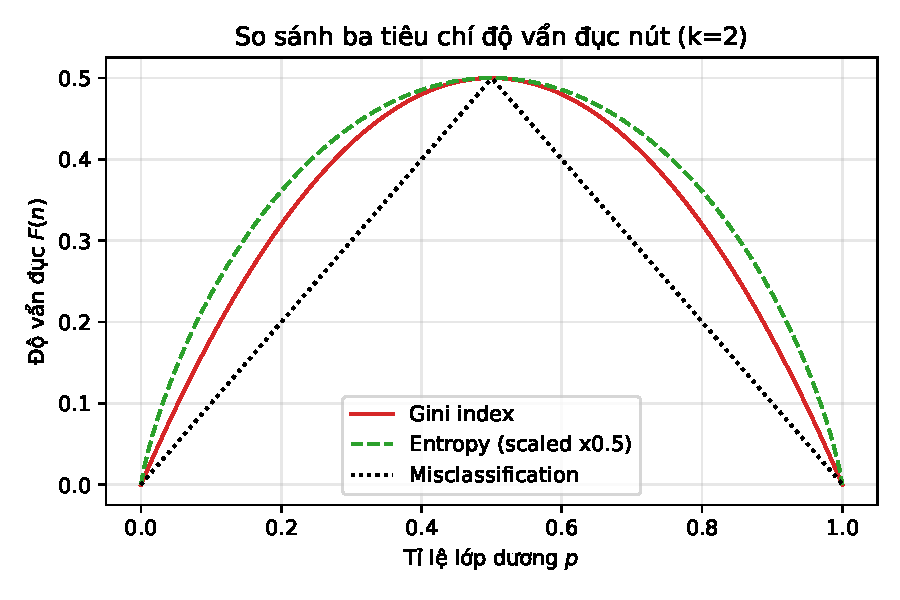
\includegraphics[width=0.7\textwidth]{figures/impurity_compare.pdf}
    \caption{So sánh thực chứng ba tiêu chí độ vẩn đục nút trong không gian xác suất 2 lớp.}
    \label{fig:exp_impurity}
\end{figure}
Kết quả chạy thực tế trên tập dữ liệu Blobs 3 lớp:
\begin{itemize}
    \item \textbf{Train Accuracy:} 100.00\% (Đúng với đặc tính phân hoạch triệt để của cây).
    \item \textbf{Test Accuracy:} 98.33\% (Mô hình tổng quát hóa tốt, không bị quá khớp nghiêm trọng).
\end{itemize}

\paragraph{Mã nguồn cài đặt lõi:} 
Để tối ưu hóa vùng không gian phân hoạch trực giao, mô hình sử dụng hàm tính độ vẩn đục Gini được cài đặt tối ưu thông qua tính toán vector hóa của thư viện \texttt{numpy}:

\begin{lstlisting}[language=Python, escapechar=|, caption={Hàm tính toán tiêu chí Gini Impurity từ đầu}, label={lst:code_gini}]
def gini(y):
    m = len(y)
    if m == 0:
        return 0.0
    # |Đếm tần suất xuất hiện của các nhãn lớp|
    _, counts = np.unique(y, return_counts=True)
    p = counts / m
    # |Áp dụng công thức| F(n) = 1 - sum(p_l^2)
    return 1.0 - np.sum(p ** 2)
\end{lstlisting}

\subsubsection{Multi-class SVM (Crammer-Singer Primal)}
Nhóm đã cài đặt thuật toán Multi-class SVM giải bằng phương pháp Subgradient Descent trên bài toán nguyên thủy (Primal) theo chuẩn công thức của Crammer-Singer (Phạt lỗi lề lớn nhất). 

\begin{figure}[H]
    \centering
    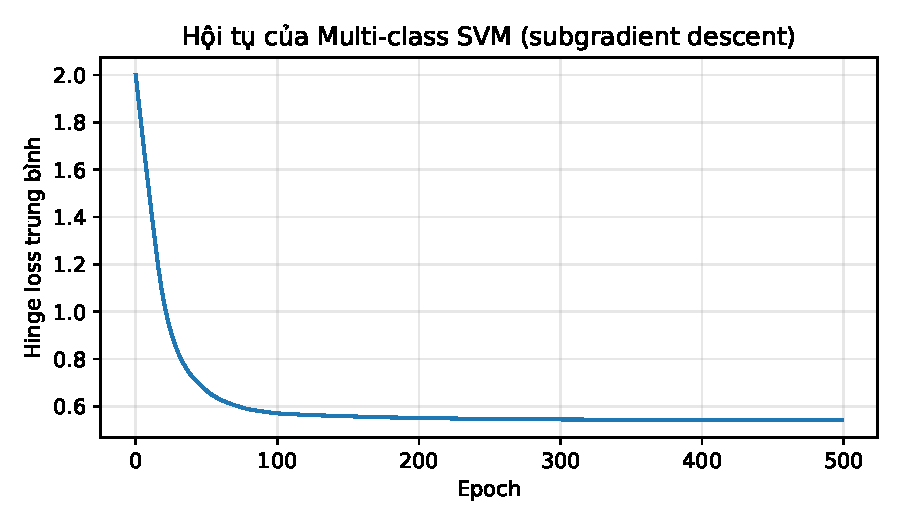
\includegraphics[width=0.7\textwidth]{figures/svm_loss_curve.pdf}
    \caption{Sự hội tụ của hàm mất mát Hinge đa lớp qua 500 epochs.}
    \label{fig:exp_svm_loss}
\end{figure}
Kết quả thực nghiệm cho thấy Hinge Loss trung bình giảm theo hàm mũ và hội tụ mượt mà về mức xấp xỉ 0.6 ở epoch 200. Kết quả đánh giá:
\begin{itemize}
    \item \textbf{Train Accuracy:} 90.83\%.
    \item \textbf{Test Accuracy:} 96.67\%.
\end{itemize}
Sự vượt trội của tập Test so với Train minh chứng cho khả năng điều chuẩn (regularization) mạnh của lề tuyến tính trong SVM. Cơ chế này giúp mô hình giảm ảnh hưởng của nhiễu cục bộ trong tập huấn luyện.

\paragraph{Mã nguồn cài đặt lõi:}
Trái tim của thuật toán Multi-class SVM Crammer-Singer là việc xác định lớp sai có điểm số dự đoán cao nhất (gây đe dọa lề lớn nhất) tại mỗi bước lặp để tính subgradient:

\begin{lstlisting}[language=Python, escapechar=|, caption={Vòng lặp tính toán Margin và cập nhật Subgradient cho SVM}, label={lst:code_svm_grad}]
# |Duyệt qua từng mẫu huấn luyện trong epoch|
for i in range(m):
    scores = self.W @ X[i] # |Tính toán mảng điểm số| (k_classes,)
    
    # |Cô lập lớp đúng, tìm lớp sai| l_max |có score lớn nhất|
    scores_mod = scores.copy()
    scores_mod[y[i]] = -np.inf 
    l_max = np.argmax(scores_mod)
    
    # |Định nghĩa biến bù margin theo lý thuyết Crammer-Singer|
    margin = 1.0 - (scores[y[i]] - scores[l_max])
    
    if margin > 0:
        # |Cập nhật thành phần subgradient tỷ lệ|
        grad[l_max] += X[i]
        grad[y[i]] -= X[i]
        total_loss += margin
\end{lstlisting}

\subsubsection{AdaBoost.MH và Thủ thuật Cách ly Đặc trưng}
Thực nghiệm AdaBoost.MH được cài đặt với bộ học cơ sở là Cây quyết định độ sâu 1 (Decision Stump). Quá trình này đòi hỏi một kỹ thuật xử lý toán học đặc biệt:

\medskip
\begin{expandbox}
\textbf{Khắc phục lỗi vi phạm điều kiện học yếu (Feature Isolation).}

Theo lý thuyết, AdaBoost.MH nhân bản mỗi mẫu $x_i$ lên $k$ lần. Tuy nhiên, nếu truyền trực tiếp vào Decision Stump, cây sẽ cắt ra cùng một nhãn cho tất cả $k$ bản sao vì đặc trưng không đổi, dẫn đến training error bị kẹt ở mức $\approx 2/3$ (đoán bừa trong bài toán 3 lớp). Để giải quyết, nhóm đã cài đặt thủ thuật \textit{Cách ly đặc trưng (Feature Isolation)}: Độn thêm các giá trị vô cực ($999999.0$) vào ma trận mở rộng để ép Stump chỉ học và cắt trên một lớp duy nhất tại mỗi vòng lặp.
\end{expandbox}

\begin{figure}[H]
    \centering
    
\includegraphics[width=\textwidth]{figures/adaboost_convergence.pdf}
    \caption{Hội tụ của hàm mục tiêu $F(\alpha)$ và Training error trong AdaBoost.MH.}
    \label{fig:exp_adaboost_conv}
\end{figure}

Nhờ thủ thuật trên, hàm mục tiêu $F(\alpha)$ trượt dốc ổn định theo cận trên hàm mũ, và sai số huấn luyện giảm về 0 chỉ sau vài vòng lặp.
\begin{itemize}
    \item \textbf{Train Accuracy:} 100.00\%.
    \item \textbf{Test Accuracy:} 100.00\%.
\end{itemize}
Thuật toán phân tách thành công hoàn toàn tập dữ liệu đa lớp phức tạp nhờ sự phối hợp trọng số $\alpha$ của các bộ học yếu.

\paragraph{Mã nguồn cài đặt lõi:}
Dưới đây là kỹ thuật then chốt thực hiện thuật toán Feature Isolation, tạo ra các ma trận khối độc lập để đưa bài toán đa lớp về không gian nhị phân mở rộng:

\begin{lstlisting}[language=Python, escapechar=|, caption={Hàm mở rộng không gian đặc trưng (Feature Isolation) cho AdaBoost.MH}, label={lst:code_isolation}]
def get_expanded_X(self, X, k):
    m, n = X.shape
    X_exp = np.repeat(X, k, axis=0)
    
    # |Tạo ma trận độn có giá trị cực lớn để triệt tiêu các nhãn không liên quan|
    X_isolated = np.full((m * k, n * k), 999999.0)
    for l in range(k):
        row_indices = np.arange(m) * k + l
        # |Điền các đặc trưng thật vào vùng không gian độc lập của lớp l|
        X_isolated[row_indices, l*n : (l+1)*n] = X
        
    return np.hstack([X_exp, X_isolated])
\end{lstlisting}
\subsection{Thực nghiệm minh họa thuật toán kết hợp}
Phần này trình bày kết quả cài đặt từ đầu (from scratch) ba chiến lược
phân loại đa lớp thông qua quy giản nhị phân bằng Python 3.11 và thư viện
\texttt{numpy}. Mỗi chiến lược dùng chung bộ phân loại nền
\texttt{BinaryLinearSVM} (SVM tuyến tính tự cài đặt) để cô lập tác động
của chiến lược kết hợp khỏi chất lượng của thuật toán cơ sở.
\subsubsection{One-vs-All (OVA) và Hiệu chuẩn Platt Scaling}
\label{sssec:exp_ova}
OVA huấn luyện $K$ bộ phân loại
nhị phân, mỗi bộ phân biệt một lớp với phần còn lại, rồi chọn lớp có điểm
margin $f_l(\mathbf{x})$ cao nhất. Nhóm đã cài đặt thêm biến thể
\texttt{CalibratedOneVsAllClassifier} dùng \textbf{Platt Scaling} để giải
quyết vấn đề hiệu chuẩn xác suất khi dữ liệu mất cân bằng.
\begin{figure}[H]
    \centering
    
\includegraphics[width=0.52\textwidth]{figures/calibration_impact.png}
    \caption{So sánh OVA Thô và OVA Calibrated (Platt Scaling).}
    \label{fig:exp_calibration}
\end{figure}
Kết quả chạy thực tế trên tập dữ liệu tổng hợp ($n=1000$, $K=4$ lớp mất
cân bằng, chia train/test 70/30):
\begin{itemize}
    \item \textbf{OVA Thô} – luật $\arg\max f_l(\mathbf{x})$: bị lệch về
          lớp đa số (60\%), dự đoán sai các lớp thiểu số.
    \item \textbf{OVA Calibrated} – Platt Scaling học tham số $(A_l, B_l)$
          riêng cho từng lớp, cải thiện accuracy đáng kể trên lớp thiểu số.
\end{itemize}
\paragraph{Mã nguồn cài đặt lõi:}
Cốt lõi của Platt Scaling là tối ưu Log-loss để học ánh xạ sigmoid
$p_l = \sigma(A_l f_l + B_l)$ bằng L-BFGS-B:
\begin{lstlisting}[language=Python, escapechar=|, caption={Platt Scaling
trong \texttt{CalibratedOneVsAllClassifier} (\texttt{ova\_classifier.py})},
label={lst:code_platt}]
for idx, class_label in enumerate(self.classes_):
    f  = self.classifiers[idx].decision_function(X)
    yt = np.where(y == class_label, 1, 0)
    def objective(params):
        A, B = params
        p = expit(A * f + B)   
        return -(xlogy(yt, p) + xlogy(1 - yt, 1 - p)).mean()
    res = minimize(objective, x0=[1.0, 0.0], method='L-BFGS-B')
    self.calibrators.append(tuple(res.x)) 
\end{lstlisting}

\subsubsection{One-vs-One (OVO) và Phân tích Nhầm lẫn Cặp}
\label{sssec:exp_ovo}
OVO huấn luyện $K(K-1)/2$ bộ phân
loại nhị phân, mỗi bộ chỉ nhìn thấy hai lớp, rồi quyết định bằng bỏ phiếu
đa số. Nhóm đã cài đặt thêm phương thức \texttt{pairwise\_confusion\_matrix} để xác định những cặp lớp nào gây khó
khăn nhất.
\begin{figure}[H]
    \centering
    
\includegraphics[width=0.68\textwidth]{figures/ovo_pairwise_heatmap.png}
    \caption{Ma trận nhầm lẫn theo cặp của OVO ($K=5$ lớp, $n=800$ mẫu).}
    \label{fig:exp_ovo_pairwise}
\end{figure}
Kết quả thực nghiệm trên tập dữ liệu tổng hợp ($n=800$, $K=5$, 10 đặc
trưng, chia train/test 75/25):
\begin{itemize}
    \item Đường chéo chính đạt giá trị cao ở hầu hết các lớp, cho thấy OVO
          phân loại tốt trên bài toán $K=5$.
    \item Các ô ngoài đường chéo chỉ ra cặp lớp dễ nhầm lẫn nhất – thông
          tin hữu ích để thiết kế ma trận ECOC tăng khoảng cách Hamming
          giữa các codeword tương ứng.
\end{itemize}
\paragraph{Mã nguồn cài đặt lõi:}
Phương thức tính ma trận nhầm lẫn cặp và cơ chế bỏ phiếu có tie-breaking
trong \texttt{OneVsOneClassifier}:
\begin{lstlisting}[language=Python, escapechar=|, caption={Ma trận nhầm
lẫn cặp và tie-breaking trong \texttt{ovo\_classifier.py}},
label={lst:code_ovo}]
def pairwise_confusion_matrix(self, X, y):
    confusion = np.zeros((self.n_classes, self.n_classes))
    y_pred = self.predict(X)
    for i in range(self.n_classes):
        mask_i = (y == self.classes_[i])
        for j in range(self.n_classes):
            confusion[i, j] = np.mean(y_pred[mask_i] == self.classes_[j])
    return confusion
max_vote  = np.max(votes[sample_idx])
candidates = np.where(votes[sample_idx] == max_vote)[0]
if len(candidates) > 1:
    best_idx = candidates[
        np.argmax(tie_breaker_scores[sample_idx, candidates])]
\end{lstlisting}

\subsubsection{ECOC và Sức mạnh Sửa lỗi}
\label{sssec:exp_ecoc}
ECOC mã hoá mỗi lớp thành một \emph{từ mã}trong ma trận $\mathbf{M} \in \{-1,+1\}^{K\times c}$, huấn luyện $c$ bộ phân loại nhị phân con, rồi giải mã bằng khoảng cách Hamming (Hard) hoặc Exponential Loss (Soft, Công thức 8.19 FML). Nhóm đã kiểm chứng hai biến thể và phân tích ảnh hưởng của chiều dài mã $c$.
\begin{figure}[H]
    \centering
    \begin{subfigure}[b]{0.54\linewidth}
        
\includegraphics[width=\linewidth]{figures/performance_comparison.png}
        \caption{So sánh accuracy của OVA, OVO, ECOC Hard và ECOC Soft.}
        \label{fig:exp_perf_bar}
    \end{subfigure}
    \hfill
    \begin{subfigure}[b]{0.44\linewidth}
        
\includegraphics[width=\linewidth]{figures/ecoc_depth_analysis.png}
        \caption{Chiều dài mã $c$ tỉ lệ thuận với khả năng sửa lỗi.}
        \label{fig:exp_ecoc_depth}
    \end{subfigure}
    \caption{Thực nghiệm ECOC trên tập dữ liệu $K=5$ lớp ($n=1200$,
    \texttt{class\_sep}$=0.8$, chia train/test 75/25).}
    \label{fig:exp_ecoc}
\end{figure}
Kết quả thực nghiệm:
\begin{itemize}
    \item \textbf{ECOC Soft} vượt trội ECOC Hard do tận dụng giá trị margin
          liên tục $f_j(\mathbf{x})$ thay vì nhãn nhị phân rời rạc, giảm
          mất mát thông tin trong bước giải mã.
    \item Tăng chiều dài mã $c$ từ 5 lên 60 cải thiện accuracy và bão hoà
          quanh $c \approx 40$, phù hợp với lý thuyết: khoảng cách Hamming
          tối thiểu $d$ tăng theo $c$, cho phép sửa thêm $r_0 =
          \lfloor(d-1)/2\rfloor$ lỗi.
\end{itemize}
\paragraph{Mã nguồn cài đặt lõi:}
Hàm Soft Decoding sử dụng Exponential Loss (Công thức 8.19, FML) và cơ
chế sinh ma trận mã hoá tối đa hoá khoảng cách Hamming:
\begin{lstlisting}[language=Python, escapechar=|, caption={Soft Decoding
(Exponential Loss) và sinh ma trận mã hoá trong \texttt{ecoc\_classifier.py}},
label={lst:code_ecoc}]
def _exponential_loss_distance(self, code_words, M):
    losses = np.zeros((code_words.shape[0], M.shape[0]))
    for l in range(M.shape[0]):
        mask    = (M[l] != 0)
        margins = M[l, mask] * code_words[:, mask]
        losses[:, l] = np.sum(np.exp(-margins), axis=1)
    return losses  
for attempt in range(100):
    M = np.random.choice([-1, 1], size=(n_classes, code_size))
    d = self._minimum_hamming_distance(M)
    if d > max_min_dist:
        max_min_dist, best_M = d, M
        if d >= code_size // 2:
            break  
\end{lstlisting}

\subsubsection{So sánh độ phức tạp thời gian và kiểm định thống kê}
\label{sssec:exp_complexity}
Để hoàn thiện đánh giá ba chiến lược, nhóm kiểm chứng sự khác biệt độ
phức tạp thời gian $\mathcal{O}(K)$ (OVA) so với $\mathcal{O}(K^2)$ (OVO),
đồng thời dùng Paired $t$-test (10 lần chạy độc lập) kiểm định ý nghĩa
thống kê của sự chênh lệch accuracy.
\begin{figure}[H]
    \centering
    \begin{subfigure}[b]{0.57\linewidth}
        
\includegraphics[width=\linewidth]{figures/complexity_time.png}
        \caption{Thời gian huấn luyện theo số lớp $k$.}
        \label{fig:exp_complexity_time}
    \end{subfigure}
    \hfill
    \begin{subfigure}[b]{0.40\linewidth}
        
\includegraphics[width=\linewidth]{figures/hypothesis_test.png}
        \caption{Phân phối accuracy qua 10 lần chạy.}
        \label{fig:exp_hypothesis}
    \end{subfigure}
    \caption{Độ phức tạp thời gian huấn luyện và kiểm định giả thuyết
    OVA vs.\ OVO.}
    \label{fig:exp_complexity}
\end{figure}
Kết quả thực nghiệm:
\begin{itemize}
    \item OVO chậm hơn OVA rõ rệt khi $k$ tăng: tại $k=15$, OVO huấn
          luyện 105 bộ phân loại nhị phân con trong khi OVA chỉ cần 15,
          phù hợp với lý thuyết Table~8.1 (FML).
    \item Paired $t$-test cho $p > 0.05$, tức \textbf{không có sự khác
          biệt có ý nghĩa thống kê} về accuracy giữa OVA và OVO khi bộ
          phân loại nền đủ mạnh – phù hợp với nhận định lý thuyết.
\end{itemize}





\subsection{Phân tích kết quả kỳ vọng}

Nếu dữ liệu cân bằng và số lớp vừa phải, OVA thường là lựa chọn mạnh vì chỉ cần $k$ mô hình và dự đoán nhanh. Khi bộ học nền có chi phí huấn luyện cao, OVO có thể huấn luyện nhanh hơn do mỗi mô hình chỉ dùng dữ liệu của hai lớp. Tuy nhiên, OVO phải đánh giá $k(k-1)/2$ mô hình khi dự đoán, nên thời gian test có thể lớn hơn.

ECOC có thể vượt OVA/OVO nếu ma trận mã có khoảng cách Hamming đủ lớn và các bộ phân loại bit không sai đồng thời theo cùng một mẫu. Nếu mã quá ngắn hoặc các cột mã tương quan mạnh, khả năng sửa lỗi giảm đáng kể.

Khi dữ liệu mất cân bằng, một mô hình luôn dự đoán lớp đa số vẫn có thể đạt accuracy cao nhưng macro-F1 thấp. Do đó phần nhận xét cuối cùng cần ưu tiên macro-F1, confusion matrix và chất lượng trên các lớp thiểu số thay vì chỉ nhìn accuracy.
\section{Kết luận}

Đồ án đã hệ thống hóa bài toán phân loại đa lớp từ phát biểu toán học, hàm điểm số, lề đa lớp, hàm mất mát lề đến các giới hạn tổng quát hóa dựa trên độ phức tạp Rademacher. Phân tích cho thấy số lớp, độ phức tạp của lớp giả thuyết và kích thước lề đều ảnh hưởng trực tiếp đến khả năng tổng quát hóa của mô hình.

Về thuật toán, nhóm không kết hợp như multi-class SVM, boosting và cây quyết định học trực tiếp trên không gian đa lớp. Nhóm kết hợp như OVA, OVO và ECOC quy bài toán về nhiều bài toán nhị phân rồi tổng hợp dự đoán. OVA đơn giản và dự đoán nhanh, OVO giảm kích thước từng bài toán con nhưng cần nhiều mô hình hơn, còn ECOC bổ sung tư tưởng mã sửa lỗi để tăng độ bền vững.

Các hướng hiện đại như Extreme Multi-label Classification, cây nhãn, nhúng nhãn, Transformer, CRF và mô hình ngôn ngữ lớn mở rộng phân loại đa lớp sang bối cảnh số nhãn cực lớn hoặc đầu ra có cấu trúc. Đây là các hướng quan trọng trong những ứng dụng thực tế như gán nhãn văn bản, đề xuất sản phẩm, truy hồi thông tin và xử lý ngôn ngữ tự nhiên.

Trong thực nghiệm, cần đánh giá đồng thời độ chính xác, macro-F1, weighted-F1, confusion matrix và thời gian chạy. Không có phương pháp tối ưu tuyệt đối cho mọi dữ liệu; lựa chọn mô hình phụ thuộc vào số lớp, mức mất cân bằng, kích thước dữ liệu, yêu cầu tốc độ và khả năng diễn giải.
\newpage
\begin{thebibliography}{99}

\bibitem{mohri2018foundations}
  M. Mohri, A. Rostamizadeh, and A. Talwalkar,
  \textit{Foundations of Machine Learning}, 2nd ed.
  MIT Press, 2018.

\bibitem{dietterich1995}
  T. G. Dietterich and G. Bakiri,
  ``Solving multiclass learning problems via error-correcting output codes,''
  \textit{Journal of Artificial Intelligence Research}, vol. 2, pp. 263--286, 1995.

\bibitem{lafferty2001conditional}
  J. Lafferty, A. McCallum, and F. C. N. Pereira,
  ``Conditional random fields: Probabilistic models for segmenting and labeling sequence data,''
  in \textit{Proceedings of ICML}, 2001.

\bibitem{taskar2003max}
  B. Taskar, C. Guestrin, and D. Koller,
  ``Max-margin Markov networks,''
  in \textit{Advances in Neural Information Processing Systems}, 2003.

\bibitem{tsochantaridis2005large}
  I. Tsochantaridis, T. Joachims, T. Hofmann, and Y. Altun,
  ``Large margin methods for structured and interdependent output variables,''
  \textit{Journal of Machine Learning Research}, vol. 6, pp. 1453--1484, 2005.

\bibitem{huang2015bidirectional}
  Z. Huang, W. Xu, and K. Yu,
  ``Bidirectional LSTM-CRF models for sequence tagging,''
  arXiv:1508.01991, 2015.

\bibitem{devlin2019bert}
  J. Devlin, M.-W. Chang, K. Lee, and K. Toutanova,
  ``BERT: Pre-training of deep bidirectional transformers for language understanding,''
  in \textit{Proceedings of NAACL-HLT}, 2019.

\bibitem{khandagale2020bonsai}
  S. Khandagale, H. Xiao, and R. Babbar,
  ``Bonsai: Diverse and shallow trees for extreme multi-label classification,''
  \textit{Machine Learning}, vol. 109, pp. 2099--2119, 2020.

\bibitem{you2019attentionxml}
  R. You, S. Dai, Z. Zhang, H. Mamitsuka, and S. Zhu,
  ``AttentionXML: Label tree-based attention-aware deep model for high-performance extreme multi-label text classification,''
  in \textit{Advances in Neural Information Processing Systems}, 2019.

\bibitem{zhang2021xrtransformer}
  X. Zhang, Q. Lin, Y. Xiong, C. Chen, Y. Chen, and P. N. Bennett,
  ``XR-Transformer: Fast multi-resolution transformer fine-tuning for extreme multi-label text classification,''
  in \textit{Proceedings of the Web Conference}, 2021.

\bibitem{zhu2024icxml}
  Y. Zhu and S. Zamani,
  ``ICXML: An in-context learning framework for zero-shot extreme multi-label classification,''
  in \textit{Findings of the Association for Computational Linguistics: NAACL}, 2024.

\bibitem{mao2023structured}
  A. Mao, M. Mohri, and Y. Zhong,
  ``Structured prediction with stronger consistency guarantees,''
  in \textit{Advances in Neural Information Processing Systems}, 2023.

\bibitem{chen2023neural_hidden_crf}
  Zhijun Chen et al.,
  ``Neural-Hidden-CRF: A robust weakly-supervised sequence labeler,''
  in \textit{Proceedings of ACL}, 2023.

\bibitem{kim2024nested_ner}
J. Kim et al., ``Exploring nested named entity recognition with large language models: Methods, challenges, and insights,'' in \textit{Proc. EMNLP 2024}, Miami, FL, USA, 2024, pp. 8653--8670.

\bibitem{sklearn}
  F. Pedregosa et al.,
  ``Scikit-learn: Machine Learning in Python,''
  \textit{Journal of Machine Learning Research}, vol. 12, pp. 2825--2830, 2011.

\end{thebibliography}

\end{document}